% Comment for anonymization
% Add preprint option for the extended version
% Also look for "SHORT" comments
% \def\fullversion{}

\documentclass{sigplanconf}

% Structure:
%
%    Abstract                              1c
% 1) Intro                                 3c
% 2) The Potential Method                  1c
% 3) Compositional Resource-Bound Analysis 4c
%    - Gulwani/ examples
% 4) Derivation Rules                      2c
% 5) Automatic Inference via LP Solving    2c
% 6) Logical State and User Interaction    2c
% 7) Soundness Proof                       2c
%    1) Cost Semantics for Clight
%    2) Quantitative Hoare Logic
% 8) Experimental Evaluation               2c
% 9) Related Work                          1c
% a) Conclusion                            1c



\newcommand{\iffull}[2]{\ifx\fullversion\undefined{#2}\else{#1}\fi}
\newcommand{\ifshort}[2]{\ifx\fullversion\undefined{#1}\else{#2}\fi}

\newcommand{\itemskip}[0]{\ifshort{\vspace{-3pt}}{}}
\newcommand{\itemskipIn}[0]{\ifshort{\vspace{-1pt}}{}}
\newcommand{\sectskip}[0]{\ifshort{\vspace{-3pt}}{}}
\newcommand{\paraskip}[0]{\ifshort{\vspace{-4pt}}{}}
\newcommand{\lstskip}[0]{\ifshort{\vspace{-2pt}}{}}
\newcommand{\aftersectskip}[0]{\ifshort{\vspace{-1pt}}{}}
\newcommand{\subsectskip}[0]{\ifshort{\vspace{-1pt}}{}}

%SHORT
%\usepackage[normal,belowskip=-11pt,aboveskip=1pt]{caption} %Remove extra space around captions
%\DeclareCaptionFormat{myformat}{#1#2#3\vspace{-4pt}\hrulefill}
%\captionsetup[figure]{format=myformat}
%\captionsetup[table]{format=myformat}
%\renewcommand{\captionlabelfont}{\bf}
%SHORT

\usepackage[utf8]{inputenc} %for utf8 input
\usepackage{amssymb} %for shift symbol
\usepackage{amsmath}
\usepackage{listings} %for code
\lstset{moredelim=[is][\color{blue}]{@}{@},keepspaces=true}
\usepackage{mathpartir} %for typing rules
\usepackage{microtype} %better micro typing
\usepackage{stmaryrd} %for llbracket
\usepackage{mathabx} % for boxes
\usepackage{graphicx} %to include png images
\usepackage{xcolor} %for colors
\usepackage{url}
\usepackage{enumitem}
\usepackage{array} %for stupid tables

%----------------------------------------------------

\usepackage{prettyref}
\newcommand{\pref}[1]{\prettyref{#1}}
\newcommand{\Pref}[1]{\prettyref{#1} \vpageref[]{#1}}
\newcommand{\ppref}[1]{\vpageref[]{#1}}
\newrefformat{fig}{Figure~\ref{#1}}
\newrefformat{app}{Appendix~\ref{#1}}
\newrefformat{tab}{Table~\ref{#1}}
\newrefformat{cha}{Challenge~\ref{#1}}
\newrefformat{compiler}{Point~\ref{#1} of \pref{thm:compiler}}

%----------------------------------------------------

\usepackage{amsthm}
\newtheorem{lemma}{Lemma}
\newtheorem{corollary}{Corollary}
\newtheorem{theorem}{Theorem}
\newtheorem{proposition}{Proposition}

%----------------------------------------------------

\lstset{
   numbers=none, %use numbers=left
   numberstyle=\tiny,
   stepnumber=1,
   numbersep=5pt,
   basicstyle=\tt\small,
   escapechar=\#,
   mathescape,
%   language=CaML,
   columns=flexible,
%   basewidth=0.455em,
   xleftmargin=\leftmargini,
%   xrightmargin=\leftmargini,
%   morekeywords={mod,div,matchD},
   deletekeywords={as},
   literate={<-}{$\;\leftarrow\;\;\,$}{3} {->}{$\;\rightarrow\;\;\,$}{3},
   firstnumber=auto % use name=NAME to identify split listings
%
% Placement: belowskip,aboveskip,lineskip,boxpos=l|c|r
%
% wonna figure-style listings? Use: caption={Useless code,label=useless
%
% keywordstyle=\color{black}\bfseries\underbar
% morekeywords={one,two,three,four}
}
% \lstinline!! 
% use basicstyle=\small ?

%How many languages are there in CompCert?
\newcommand{\howmanylanguages}[0]{11}

%How many passes are there in CompCert?
\newcommand{\howmanypasses}[0]{20}

\newcommand{\lines}[1]{\textsl{{\scriptsize #1}}}

\newcommand{\toolname}[0]{\ensuremath{C^4\!B} }

\newcommand{\valid}[6]{\ensuremath{\mathit{valid}(#1,#2,#3,#4,#5,#6)}}
\newcommand{\validC}[2]{\ensuremath{\mathit{validC}(#1,#2)}}
\newcommand{\safe}[4]{\ensuremath{\mathit{safe}(#1,#2,#3,#4)}}
\newcommand{\safeK}[5]{\ensuremath{\mathit{safeK}(#1,#2,#3,#4,#5)}}

\newcommand{\refines}[0]{\ensuremath{\prec}}

\newcommand{\qrefines}[0]{\ensuremath{\mathop{\prec_Q}}}

\newcommand{\pruned}[1]{\ensuremath{\overline{ #1} }}

\newcommand{\sem}[1]{\ensuremath{\llbracket #1 \rrbracket}}

\newcommand{\progs}[0]{\ensuremath{\mathcal{P}}}

\newcommand{\id}[0]{\ensuremath{\mathit{x}}}

\newcommand{\xevent}[0]{\ensuremath{\nu}}
\newcommand{\cevent}[0]{\ensuremath{\mu}}
\newcommand{\event}[0]{\ensuremath{\iota}}

\newcommand{\evalue}[0]{\ensuremath{v}}

\newcommand{\intval}[1]{\ensuremath{\mathsf{int}(#1)}}

\newcommand{\floatval}[1]{\ensuremath{\mathsf{float}(#1)}}

\newcommand{\call}[1]{\ensuremath{\mathsf{call}(#1)}}
\newcommand{\return}[1]{\ensuremath{\mathsf{ret}(#1)}}
\newcommand{\malloc}[1]{\ensuremath{\mathsf{malloc}(#1)}}
\newcommand{\free}[1]{\ensuremath{\mathsf{free}(#1)}}

\newcommand{\trace}[0]{\ensuremath{t}}

\newcommand{\Trace}[0]{\ensuremath{T}}

\newcommand{\conv}[2]{\ensuremath{\mathsf{conv}(#1,#2)}}

\newcommand{\divt}[1]{\ensuremath{\mathsf{div}(#1)}}

\newcommand{\fail}[1]{\ensuremath{\mathsf{fail}(#1)}}

\newcommand{\behav}[0]{\ensuremath{B}}

\newcommand{\getchar}[0]{\ensuremath{\mathsf{getchar}}}

\newcommand{\Z}[0]{\ensuremath{\mathbb{Z}}}
\newcommand{\N}[0]{\ensuremath{\mathbb{N}}}
\newcommand{\Qplusz}[0]{\ensuremath{\mathbb Q^+_0}}
\newcommand{\Q}[0]{\ensuremath{\mathbb{Q}}}

\newcommand{\weight}[2]{\ensuremath{W_{#2}(#1)}}
\newcommand{\tval}[2]{\ensuremath{V_{#2}(#1)}}

\newcommand{\prefs}[1]{\ensuremath{\mathit{prefs}(#1)}}

\newcommand{\type}[1]{\ensuremath{\mathsf{#1}}}

\newcommand{\code}[1]{\ensuremath{\mathsf{#1}}}

\newcommand{\env}[0]{\ensuremath{\mathit{\theta}}}

\newcommand{\mem}[0]{\ensuremath{\mathit{H}}}

\newcommand{\Mem}[0]{\ensuremath{\mathit{Mem}}}

\newcommand{\Var}[0]{\ensuremath{\mathit{Var}}}

\newcommand{\Val}[0]{\ensuremath{\mathit{Val}}}

\newcommand{\Aux}[0]{\ensuremath{\mathit{Aux}}}

\newcommand{\Input}[0]{\ensuremath{\mathit{StdIn}}}

\newcommand{\Assn}[0]{\ensuremath{\mathit{Assn}}}
\newcommand{\State}[0]{\ensuremath{\mathit{State}}}
\newcommand{\state}[0]{\ensuremath{\sigma}}

\newcommand{\Prop}[0]{\ensuremath{\mathit{Prop}}}

\newcommand{\ret}[0]{\ensuremath{\mathit{ret}}}

\newcommand{\htriple}[3]{\ensuremath{\{#1\}\, #2\, \{#3\}}}

\newcommand{\smallstep}[1]{\ensuremath{\to_{#1}}}

\newcommand{\conform}[2]{\ensuremath{\mathit{agree}(#1,#2)}}

\newcommand{\dom}[1]{\ensuremath{ \text{dom}(#1)}}
\newcommand{\img}[1]{\ensuremath{ \text{img}(#1)}}

\newcommand{\pimp}[2]{\ensuremath{#1 \Rightarrow #2}}

\newcommand{\Assert}[0]{\ensuremath{\mathit{Assert}}}

\newcommand{\VAssert}[0]{\ensuremath{\mathit{VAssert}}}

\newcommand{\eenv}[0]{\ensuremath{\Sigma}}

\newcommand{\genv}[0]{\ensuremath{\Delta}}

\newcommand{\fenv}[0]{\ensuremath{\Sigma}}

\newcommand{\Fundef}[0]{\ensuremath{\mathit{Fundef}}}

\newcommand{\funs}[0]{\ensuremath{\mathit{FID}}}

\newcommand{\vars}[0]{\ensuremath{\mathit{VID}}}

\newcommand{\statements}[0]{\ensuremath{\mathcal{S}}}

\newcommand{\traces}[0]{\ensuremath{\mathcal{T}}}

\newcommand{\behavs}[0]{\ensuremath{\mathcal{B}}}

\newcommand{\events}[0]{\ensuremath{\mathcal{E}}}

\newcommand{\initState}[2]{\ensuremath{\mathit{initSt}(#1,#2)}}

\newcommand{\retState}[1]{\ensuremath{\mathit{retState}(#1)}}

\newcommand{\Potential}[0]{\ensuremath{\mathit{Pot}}}

\newcommand{\evalE}[2]{\ensuremath{\llbracket #1 \rrbracket_{#2}}}

\newcommand{\Kseq}[2]{\ensuremath{\mathsf{Kseq}\, #1 \, #2}}

\newcommand{\Kloop}[2]{\ensuremath{\mathsf{Kloop}\, #1 \, #2}}

\newcommand{\Kstop}[0]{\ensuremath{\mathsf{Kstop}}}

\newcommand{\Kcall}[3]{\ensuremath{\mathsf{Kcall}\, #1 \, #2 \, #3}}

\newcommand{\cont}[0]{\ensuremath{K}}

\newcommand{\cost}[0]{\ensuremath{c}}

\newcommand{\used}[0]{\ensuremath{\sqbullet}}

\newcommand{\init}[0]{\ensuremath{\square}}

\newcommand{\FV}[1]{\ensuremath{\text{FV}(#1)}}

\newcommand{\loc}[0]{\ensuremath{\text{Loc}}}

\newcommand{\inter}[2]{\ensuremath{[#1,#2]}}

\newcommand{\ind}[0]{\ensuremath{\mathcal{I}}}

\newcommand{\states}[0]{\ensuremath{\mathcal{H}}}

\newcommand{\shift}[0]{{\lhd}}

\newcommand{\Vret}[0]{{\ensuremath{\mathit{ret}}}}
\newcommand{\Vargs}[0]{{\ensuremath{\vec {\mathit{args}}}}}

\newcommand{\tr}[0]{\ensuremath{\mathcal T}}

%-------------------------------------------------------
%Type rules (mathpatir)

\newcommand{\Rule}[4][]{\ensuremath{\inferrule*[right={\!(#2)},#1]{#3}{#4}}}
\newcommand{\RuleToplabel}[4][]{\ensuremath{\inferrule[(#2)]{#3}{#4}}}
\newcommand{\RuleNolabel}[3][]{\ensuremath{\inferrule*[#1]{#2}{#3}}}

%-------------------------------------------------------


%%% Local Variables: 
%%% mode: latex
%%% TeX-master: "main"
%%% End: 

\newcommand{\jan}[1]{{\color{orange}[[{#1}]]}}

\begin{document}

\special{papersize=8.5in,11in}
\setlength{\pdfpageheight}{\paperheight}
\setlength{\pdfpagewidth}{\paperwidth}

\conferenceinfo{PLDI'15}{, June 13--17, 2015, Portland, OR, USA}
\copyrightyear{2015}
\copyrightdata{978-1-4503-3468-6/15/06}
\doi{nnnnnnn.nnnnnnn}

\titlebanner{\iffull{Extended Version}{}}%{Draft -- Do not distribute}        % These are ignored unless
\preprintfooter{\iffull{Extended Version\hspace{-.8cm}}{Draft\hspace{.5cm}}}%{Draft}   % 'preprint' option specified.

\title{Compositional Certified Resource Bounds}
% Certified Resource Bounds for C
% Compositional Certified Resource Bounds for C
% Compositional Quantitative Resource Analysis of C Programs
% Compositional Resource-Bound Certification for C Programs

\authorinfo
{Quentin Carbonneaux \and Jan Hoffmann \and Zhong Shao}
{Yale University \vspace{-1cm}}

\maketitle


%SHORT
\ifx\fullversion\undefined
\abovedisplayskip=3pt
\belowdisplayskip=3pt
\abovedisplayshortskip=3pt
\belowdisplayshortskip=3pt
\else
\fi
%SHORT

%----------------------------------------------------



\begin{abstract}
  This paper presents a new approach for automatically deriving
  worst-case resource bounds for C programs.
  %
  The described technique combines ideas from amortized analysis and
  abstract interpretation in a unified framework to address four
  challenges for state-of-the-art techniques: compositionality, user
  interaction, generation of proof certificates, and scalability.
  %
  \emph{Compositionality} is achieved by incorporating the potential
  method of amortized analysis.  It enables the derivation of global
  whole-program bounds with local derivation rules by naturally
  tracking size changes of variables in sequenced loops and function
  calls.  The resource consumption of functions is described abstractly
  and a function call can be analyzed without access to the function
  body.
  %\
  \emph{User interaction} is supported with a new mechanism that
  clearly separates qualitative and quantitative verification. A user
  can guide the analysis to derive complex non-linear bounds by using
  auxiliary variables and assertions.  The assertions are
  separately proved using established qualitative techniques such as
  abstract interpretation or Hoare logic.
  %
  \emph{Proof certificates} are automatically generated from the local
  derivation rules. A soundness proof of the derivation system with
  respect to a formal cost semantics guarantees the validity of the
  certificates.
  %
  \emph{Scalability} is attained by an efficient reduction of
  bound inference to a linear optimization problem that can be solved
  by off-the-shelf LP solvers.
  %
  The analysis framework is implemented in the publicly-available
  tool $\toolname$. An experimental evaluation demonstrates the
  advantages of the new technique with a comparison of $\toolname$ with
  existing tools on challenging micro benchmarks and the analysis of
  more than $\totalLoc$ lines of C code from the cBench benchmark suite.

% Contrary to most available tools for
% C, ours has a compositional design that provides the
% programmer with bounds expressed in terms of meaningful
% variables.  The compositionality allows to handle uniformly
% nested sequenced loops and recursive sequenced function
% calls.  The automatic analysis is implemented
% as a tool that leverages state-of-the-art SMT solvers
% LP solvers to automatically infer resource bounds on
% a wide range of C programs.  It is the first automatic
% amortized analysis that can derive bounds that depend
% on negative integers and differences between numbers.
% To prove its soundness and give a concrete shape to proof
% certificates, we developed a quantitative Hoare logic
% that we proved sound using the Coq proof assistant.  This
% logic allows manual proofs of arbitrarily complex resource
% bounds on C programs and interaction with the automation.
% To prove the scalability and precision of this new tool,
% we run it on multiple code snippets from the literature,
% reproduce results from previous work, and analyze a
% consequent part of a modern benchmark suite.

%   The goal of quantitative resource analysis is to provide developers
%   with quantitative information about the runtime behavior of software
%   at development time.  Recent years have seen tremendous progress in
%   automatically deriving worst-case resource bounds, yet many
%   challenges in specifying, interactively deriving, formally
%   certifying, and composing resource bounds remain unsolved.
%
%   This paper describes a novel quantitative resource analysis
%   framework that tackles these challenges for C programs.  The
%   analysis framework consists of three parts: First, a parametric cost
%   semantics formalizes the resource consumption of CompCert Clight
%   programs.  Second, a quantitative Hoare logic enables users to
%   interactively develop resource bounds in the Coq Proof Assistant.
%   The logic is proved sound with respect to the cost semantics, and
%   shallow embedding enables a derived bound to be any function that is
%   definable in Coq.  Third, an automatic amortized resource analysis
%   for Clight computes derivations in the quantitative Hoare logic.
%   It is the first automatic amortized analysis that can derive bounds
%   that depend on negative integers or differences between numbers,
%   which is crucial to handle typical systems code.  Both, the
%   quantitative logic and the automatic amortized analysis are
%   naturally compositional and can be combined to semi-automatically
%   derive global resource bounds.
%   %
%   An experimental evaluation demonstrates the practicality of the
%   analysis framework.  The expressivity of the logic is shown by
%   manually deriving customized bounds that are tailored to specific
%   algorithms.  A comparison of the automatic amortized analysis with
%   other automatic tools on 30 challenging loop and recursion patterns
%   from the literature and open-source software shows that the bounds
%   derived by the automatic amortized analysis are often more precise.
\end{abstract}

% \category{D.2.4}{Software Engineering}
% {Software/Program Verification}
% \category{F.3.1}{Logics and Meanings of Programs}
% {Specifying and Verifying and Reasoning about Programs}

% \terms Verification, Reliability


% \keywords Formal Verification, Compiler Construction, Program Logics,
% Stack-Space Bounds, Quantitative Verification


\sectskip
\section{Introduction}
\label{sec:intro}
\aftersectskip

In software engineering and software verification,
we often would like to have static information
about the quantitative behavior of programs.
For example, stack and heap-space bounds
are important to ensure the reliability of
safety-critical systems~\cite{Regehr05}.
Static energy usage information is critical
for autonomous systems and has applications in
cloud computing~\cite{CohenZSL12,CarrollH10}.
Worst-case time bounds can help create
constant-time implementations that prevent
side-channel attacks~\cite{KasperS09,BartheBCLP14}.
Loop and recursion-depth bounds are used to
ensure the accuracy of programs that are executed
on unreliable hardware~\cite{CarbinMR13} and
complexity bounds are needed to verify cryptographic
protocols~\cite{BartheGB09}.  In general, quantitative
resource information % at design time
can provide useful
feedback for developers.




% NEW NEW NEW NEW NEW NEW NEW NEW NEW NEW NEW NEW NEW

Available techniques for {\em automatically} deriving worst-case
resource bounds fall into two categories.  Techniques in the first
category derive impressive bounds for numerical imperative programs,
but are not compositional.  This is problematic if one needs to derive
global whole-program bounds.
%%%%%%
Techniques in the second category derive
tight whole-program bounds for programs with regular loop or
recursion patterns that decrease the size of an individual variable or
data structure. They are highly compositional, scale for large
programs, and work directly on the syntax.  However,
they do not support multivariate interval-based resource bounds
(e.g., $x-y$) which are common in C programs. Indeed,
it has been a long-time open problem to develop compositional
resource analysis techniques that can work for typical imperative code
with non-regular iteration patterns, signed integers, mutation, and non-linear
control flow. % As a result, they are not suitable for
% typical imperative code.

Tools in the first category include
SPEED~\cite{GulwaniMC09}, KoAT~\cite{BrockschmidtEFFG14},
PUBS~\cite{AlbertAGPZ12}, Rank~\cite{AliasDFG10},
and LOOPUS~\cite{SinnZV14}.
They lack compositionality in at least two ways.
First, they all base their analysis on some form of
\emph{ranking function} or \emph{counter instrumentation}
that is linked to a local analysis.  As a result, loop bounds are
arithmetic expressions that depend on the values of
variables just before the loop.
This makes it hard to give a
resource bound on a sequence of loops and function calls in
terms of the input parameters of a function.
Second, while all popular imperative programming languages
provide a function or procedure abstraction, available
tools are not able to abstract resource behavior;
instead, they have to inline the procedure body to perform their
analysis.

Tools in the second category originate form the {\em potential method}
of amortized analysis and type systems for functional
programs~\cite{Jost03,HoffmannAH12}. It has been shown that class
definitions of object-oriented programs~\cite{Jost06} and
data-structure predicates of separation logic~\cite{Atkey10} can play
the role of the type system in imperative programs.
However, a major weakness of existing potential-based techniques
is that they can only associate \emph{potential}
with individual program variable or data structure.
For C programs, this
fails for loops as simple as \lstinline{for(i=x;i<y;i++)} where
$y-i$ decreases, but not $|i|$. %  Mutation is yet another problem.
% While functional programs relate multiple fixed inputs (the typing
% context) with one output (the expression typed), imperative programs
% can change the value of variables in scope, so the potential of these
% variables has to be updated after mutations to ensure soundness.

% these
% techniques fail for numerical imperative programs because they lack
% fine-grained data-structure information to hook the analysis on.
% Another issue is that existing techniques associate \emph{potential}
% directly with single program variables.

A general problem with existing tools (in both categories) is user interaction. When a tool
fails to find a resource bound for a program, there is no possibility
for sound user interaction to guide the tool during bound
derivation.
For example, there is no concept of manual proofs of
resource bounds; and no framework can support composition
of manually derived bounds with automatically inferred bounds.

% Finally, the tools often operate on an abstract version of the and use
% complex external tools from term rewriting and abstract
% interpretation. This makes it hard to generate a proof certificate for
% the bounds or even to prove the soundness of the tools with respect to
% a formal cost semantics.


This paper presents a new compositional framework for automatically
deriving resource bounds on C programs.  This new
approach is an attempt to unify the two aforementioned
categories: It solves the compositionality issues of techniques
for numerical imperative code by adapting amortized-analysis--based
techniques from the functional world.
%
Our automated analysis is able to infer
resource bounds on C programs with mutually-recursive functions and integer loops.
%
The resource behavior of functions can be summarized
in a function specification that can be used at every
call site without accessing the function body.
%
To our knowledge this is the first technique based on
amortized analysis that is able to derive bounds that depend on negative numbers
and differences of variables.  It is also the first
resource analysis technique for C that deals naturally with
recursive functions and sequenced loops, and can handle resources that can
become available during execution (e.g., when freeing
memory).  Compared to more classical
approaches based on ranking functions, our tool inherits
the benefits of amortized reasoning.  Using only one
simple mechanism, it handles:
\itemskip
\begin{itemize}
\item interactions between \emph{sequential loops or
  function calls} through size changes of variables,
\itemskipIn
\item \emph{nested loops} that influence each other
  with the same set of modified variables,
\itemskipIn
\item and \emph{amortized bounds} as found, for example, in
  the Knuth-Morris-Pratt algorithm for string search.
\end{itemize}
\itemskip
The main innovations that make amortized analysis work
on imperative languages are to base the analysis on a
Hoare-like logic and to track multivariate quantities instead
of program variables.  This leads to precise bounds
expressed as functions of sizes $|[x, y]| = \max(0, y-x)$ of
intervals.
%
A distinctive feature of our analysis system is that
it reduces linear bound inference  to a linear optimization problem
that can be solved by off-the-shelf LP solvers.  This enables the
efficient inference of global bounds for larger programs.
%
Moreover, our local inference rules automatically generate
proof certificates that can be easily checked in linear time.

The use of the potential method of amortized analysis makes user
interaction possible in different ways. For one thing, we can directly
combine the new automatic analysis with manually derived bounds in a
previously-developed quantitative Hoare logic~\cite{veristack14} (see
\pref{sec:soundness}).  For another thing, we describe a new mechanism that
allows the separation of quantitative and qualitative verification
(see \pref{sec:anno}).  Using this mechanism, the user can guide the
analysis by using auxiliary variables and logical assertions that can
be verified by existing qualitative tools such as Hoare logic or
abstract interpretation.  In this way, we can benefit from existing
automation techniques and provide a middle-ground between fully
automatic and fully manual verification for bound derivation. This
enables the semi-automatic inference of non-linear bounds, such as
polynomial, logarithmic, and exponential bounds.

We have implemented the analysis system in the tool
\toolname and experimentally evaluated its effectiveness by
analyzing system code and examples from the literature.
\toolname has automatically derived global resource bounds for
more than $\totalLoc$ lines of C code from the cBench benchmark suite.
%
\iffull{\pref{app:cat}}{The extended version
  of this article~\cite{anon_extended}}{} contains more than $30$
challenging loop and recursion patterns that we collected from open
source software and the literature.  Our analysis can find
asymptotically tight bounds for all but one of these patterns, and in
most cases the derived constant factors are tight.  To compare $\toolname$
with existing techniques, we tested our examples
with tools such as KoAT~\cite{BrockschmidtEFFG14},
Rank~\cite{AliasDFG10}, and LOOPUS~\cite{SinnZV14}.  Our experiments
show that the bounds that we derive are often more precise than those
derived by existing tools.  Only LOOPUS~\cite{SinnZV14}, which also
uses amortization techniques, is able to achieve a similar precision.

Examples from cBench and micro benchmarks demonstrate the practicality and
expressiveness of the user guided bound inference.  For example, we
derive a logarithmic bound for a binary search function\iffull{, a bound that
depends on the contents of an array to describe the exact cost of a
function that finds a maximal element in an array, }{ }and a bound
that amortizes the cost of $k$\iffull{ successive }{ }increments to a binary
counter (see \pref{sec:anno}).

In summary, we make the following \emph{contributions}.
\itemskip
\begin{itemize}
\item We develop the first automatic amortized analysis for C
  programs. It is naturally compositional, tracks size changes of
  variables to derive global bounds, can handle mutually-recursive
  functions, generates resource abstractions for functions, derives
  proof certificates, and handles resources that can
  become available during execution.
\itemskipIn
\item We show how to automatically reduce the inference of \emph{linear} resource
    bounds to efficient LP solving.
\itemskipIn
\item We describe a new method of harnessing existing qualitative
  verification techniques to guide the automatic amortized analysis
  to derive \emph{non-linear} resource bounds with LP solving.
\itemskipIn
\item We prove the soundness of the analysis with respect to a
  parametric cost semantics for C programs. The cost model can be
  further customized with function calls (\code{tick(n)}) that
  indicate resource usage. % This mechanism is also covered by the
  % soundness proof.
\itemskipIn
\item We implemented our resource bound analysis in the publicly-available tool $\toolname$.
\itemskipIn
\item We present experiments with $\toolname$ on more
  than $\totalLoc$ lines of C code. A detailed comparison shows that our
  prototype is the only tool that can derive global bounds for larger
  C programs while being as powerful as existing tools when deriving
  linear local bounds for tricky loop and recursion patterns.
\end{itemize}
\itemskip


\sectskip
\section{The Potential Method}
\aftersectskip

The idea that underlies the design of our framework is amortized
analysis~\cite{Tarjan-amort}.  Assume that a program $S$ executes
on a starting state $\state$ and consumes $n$ resource units of
some user-defined quantity.  We denote that by writing $(S, \state)
\Downarrow_n \state'$ where $\state'$ is the program state after
the execution.  The basic idea of amortized analysis is to define a
\emph{potential function} $\Phi$ that maps program states to non-negative
numbers and to show that $\Phi(\state) \geq n$ if $\state$ is a program
state such that $(S, \state) \Downarrow_n \state'$.  Then
$\Phi(\state)$ is a valid resource bound.

To obtain a compositional reasoning we also have to take into account the
state resulting from a program's execution.  We thus use two potential
functions, one that applies before the execution, and one that applies
after.  The two functions must respect the relation $\Phi(\state)
\ge n + \Phi'(\state')$ for all states $\state$ and $\state'$ such
that $(S, \state) \Downarrow_n \state'$.  Intuitively, $\Phi(\state)$
must provide enough \emph{potential} for both, paying for the resource
cost of the computation and paying for the potential $\Phi'(\state')$ on
the resulting state $\state'$. That way, if $(\state, S_1) \Downarrow_n
\state'$ and $(\state', S_2) \Downarrow_m \state''$, we get $\Phi(\state)
\ge n + \Phi'(\state')$ and $\Phi'(\state') \ge m + \Phi''(\state'')$.
This can be composed as $\Phi(\state) \ge (n + m) + \Phi''(\state'')$.
Note that the initial potential function $\Phi$ provides an upper bound
on the resource consumption of the whole program.  What we have observed
is that, if we define $\htriple{\Phi} {S}{\Phi'}$ to mean
$$
\forall \state\, n\, \state'.\, (\state, S) \Downarrow_n \state' \implies \Phi(\state) \ge
n + \Phi'(\state') \; ,
$$
then we get the following familiar looking rule
$$
\RuleNolabel
{\htriple{\Phi}{S_1}{\Phi'} \\ \htriple{\Phi'}{S_2}{\Phi''}}
{\htriple{\Phi} {S_1; S_2}  {\Phi''}} \;\; .
$$
%
This rule already shows a departure from classical techniques that are
based on ranking functions.  Reasoning with two potential functions
promotes compositional reasoning by focusing on the sequencing of
programs.  In the previous rule, $\Phi$ gives a bound for
$S_1; S_2$ through the intermediate potential $\Phi'$, even though it
was derived on $S_1$ only.
%
Similarly, other language constructs lead to rules for the potential
functions that look very similar to Hoare logic or effect system
rules.  These rules enable reasoning about resource usage
in a flexible and compositional way, which, as a side effect, produces
a certificate for the derived resource bound.


% \subsection{Automating  Amortized Analysis}

% To make amortized reasoning feasible on large code bases, we would
% like to automatically infer the potential functions.  The first step
% towards this goal is to reduce our search space by fixing the shape of
% potential functions $\Phi$.  In this paper, we focus on a form that
% can express tight bounds for many typical programs and allows
% inference view \emph{linear programming}:
% %
% $$
% \Phi(\state) = q_0 + \sum_{x,y \in \dom{\state}}
%   q_{(x,y)} \cdot |[\state(x),\state(y)]|
% $$
% where $q_{(x,y)} \in \Qplusz$ and $|[a,b]| = \max(b-a,0)$.  For now, we assume
% that a program state is a simple map from program variables to integers
% and we treat constants as program variables (that cannot be changed
% by the program text).  For instance, $q_{(0,x)}|[0,x]|$ always appear in
% the sum.  % We then develop an inference rule for each syntactic construct
% % that derives a triple $\htriple{\Phi}P{\Phi'}$ sound in the sense of
% % the previous section.


The derivation of a resource bound using potential functions is best
explained by example.  If we use the tick metric that assigns cost $n$
to the function call \code{tick(n)} and cost $0$ to all other
operations then the cost of the following example can be bounded by
$|[x,y]| = \max(y{-}x,0)$.% \footnote{Note that there are no restrictions on
  % the signs of the input variables in the examples.}
\begin{lstlisting}[basicstyle=\tt\small]
while (x<y) { x=x+1; tick(1); } #\hfill \textnormal{(Example 1)}#
\end{lstlisting}
To derive this bound, we start with the initial potential $\Phi_0 =
|[x,y]|$, which
we also use as the loop invariant.  For the loop body we have (like in
Hoare logic) to derive a triple like
$\htriple{\Phi_0}{\code{x=x+1;tick(1)}}{\Phi_0}$.  We can only do so
if we utilize the fact that $x<y$ at the beginning of the loop body.
The reasoning then works as follows. We start with the potential
$|[x,y]|$ and the fact that $|[x,y]| > 0$ before the assignment.  If
we denote the updated version of $x$ after the assignment by $x'$ then
the relation $|[x,y]| = |[x',y]| + 1$ between the potential before and
after the assignment \code{x=x+1} holds.  This means that we have the
potential $|[x,y]| + 1$ before the statement \code{tick(1)}.  Since
\code{tick(1)} consumes one resource unit, we end up with potential
$|[x,y]|$ after the loop body and have established the loop invariant
again.



\begin{figure}[t]
  \centering
\vspace{-1.5ex}
\begin{lstlisting}[mathescape]
${\color{blue}%
  \{ \cdot; \, 0 + \frac{T}{K} {\cdot} |[x,y]| + 0 {\cdot} |[y,x]| \} }$
while (x+K<=y) {
  ${\color{blue}%
  \{ x + K \le y; \; 0 + \frac{T}{K} {\cdot} |[x,y]| + 0 {\cdot} |[y,x]| \} }$
  x=x+K;
  ${\color{blue}%
  \{ x \leq y; \, T + \frac{T}{K} {\cdot} |[x,y]| + 0 {\cdot} |[y,x]| \} }$
  tick(T);
  ${\color{blue}%
  \{ x \leq y; \, 0 + \frac{T}{K} {\cdot} |[x,y]| + 0 {\cdot} |[y,x]| \} }$
}
${\color{blue}%
 \{ x \geq y; 0 + \frac{T}{K} {\cdot} |[x,y]| + 0 {\cdot} |[y,x]| \} }$
\end{lstlisting}
  \caption{Derivation of a tight bound on the number of
    ticks for a standard \emph{for loop}.  The parameters $K>0$ and
    $T>0$ are not program variables but denote concrete constants.
    % The reasoning works uniformly for all such $K$ and
    % $T$.
  }
  \label{fig:ex1}
\end{figure}

\pref{fig:ex1} shows a derivation of the bound
$\frac{T}{K}{\cdot}|[x,y]|$ on the number of ticks for a generalized
version of Example~1 in which we increment $x$ by a constant $K>0$ and
consume $T>0$ resources in each iteration.  The reasoning is similar
to the one of Example~1 except that we obtain the potential
$K{\cdot}\frac{T}{K}$ after the assignment.  Note that the logical
assertions are only used in the rule for the assignment
\code{x=x+K}.

To the best of our knowledge, no other implemented tool for C is
currently capable of deriving a tight bound on the cost of such a
loop.  For $T=1$ (many systems focus on the number of loop iterations
without a cost model) and $K=10$, KoAT computes the bound $|x| + |y| +
10$, Rank computes the bound $y-x-7$, and LOOPUS computes the bound
$y-x-9$.  Only PUBS computes the tight bound $0.1(y-x)$ if we
translate the program into a term-rewriting system by
hand. We will show in the following sections that the
potential method makes automatic bound derivation straightforward.

% To automate the reasoning, we first introduce an unknown rational
% variable for each factor in the potential functions.  We then use our
% inference rules (see \pref{sec:AAA}) to emit linear constraints on
% these variables that enforce that variable assignments that respect
% the constraints correspond to sound potential annotations.  For
% instance if $K = 1$ in \pref{fig:ex1} then we would have the
% annotation $q_0 + q_{(x,y)} {\cdot} |[x,y]| + q_{(y,x)} {\cdot}
% |[y,x]|$ before the assignment and $p_0 + p_{(x,y)} {\cdot} |[x,y]| +
% p_{(y,x)} {\cdot} |[y,x]|$ after the assignment, where $q_i$ and $p_i$
% are unknown and must satisfy constraints like $p_{(x,y)} = q_{(x,y)}$,
% $p_{(y,x)} = q_{(y,x)}$, and $p_0 = q_0 + q_{(x,y)} -
% q_{(y,x)}$. Finally, we call an off-the-shelf LP solver to minimize
% the coefficients of the initial potential function. LP solvers are
% among the most mature constraint solving tools. As a result, the bound
% derivation works very efficiently in practice.

% \iffull{It might be surprising that we}{We} only track simple linear relations in
% the logical context $\Gamma$.  While it would of course be possible to keep
% track of more sophisticated assertions, this simple form is
% sufficient for the examples we considered and we can efficiently
% decide queries such as $\Gamma \implies x<y \; ?$ that we make in the
% assignment rule.  Nevertheless, this logical part of our analysis
% system is orthogonal to the quantitative part and can be easily
% extended if necessary.

The concept of a potential function is a generalization of the
concept of a ranking function.  A potential function can be used like
a ranking function if we use the tick metric and add the statement
\code{tick(1)} to every back edge of the program (loops and function
calls).  However, a potential function is more flexible.  For example,
we can use a potential function to prove that Example~2 does not
consume any resources in the tick metric.
\begin{lstlisting}[basicstyle=\tt\small]
#\!\!\!\!\!#while (x<y) {tick(-1); x=x+1; tick(1)} #\hfill \textnormal{(Example 2)}#

#\!\!\!\!\!#while (x<y) { x=x+1; tick(10); } #\hfill \textnormal{(Example 3)}#
\end{lstlisting}
Similarly we can prove that Example~3 can be bounded by $10|[x,y]|$.
In both cases, we reason exactly like in the first version of the
while loop to prove the bound.  Of course, such loops with different
tick annotations can be seamlessly combined in a larger program.

\iffull{In general, the potential based approach addresses several challenges
in resource bound analysis. This includes amortized bounds in which
individual loop iterations have different resource consumption,
sequential loops or function calls that require the tracking of size
changes of variables, and nested loops that interact by modifying the
same set of variables.}{}

\newlength{\progwidth}

\begin{figure*}
 \setlength{\progwidth}{.22\linewidth}
  \centering
\vspace{-.3cm}
\hspace{-0.4cm}
  \begin{minipage}[b]{.18\linewidth}
    \begin{center}
   \begin{lstlisting}[]
while (n>x) {
  ${\color{blue}%
  \{ n{>}x; \, |[x, n]| {+} |[y, m]| \} }$
  if (m>y)
    ${\color{blue}%
    \{ m{>}y; \, |[x, n]| {+} |[y, m]| \} }$
    y=y+1;
    ${\color{blue}%
    \{ \cdot ; \, 1 {+} |[x, n]| {+} |[y, m]| \} }$
  else
    ${\color{blue}%
    \{ n{>}x; \, |[x, n]| {+} |[y, m]| \} }$
    x=x+1;
    ${\color{blue}%
    \{ \cdot; \, 1 {+} |[x, n]| {+} |[y, m]| \} }$
  ${\color{blue}%
  \{ \cdot; \, 1 {+} |[x, n]| {+} |[y, m]| \} }$
  tick(1);
} ${\color{blue}%
  \{ \cdot; \, |[x, n]| {+} |[y, m]| \} }$
   \end{lstlisting}
\vspace{-2.5ex}
$|[x, n]| + |[y, m]|$
\\[.4\baselineskip]
      {\bf speed\_1}
    \end{center}
  \end{minipage}
%
\hfill
%
  \begin{minipage}[b]{\progwidth}
    \begin{center}
   \begin{lstlisting}

while (x<n) {
  ${\color{blue}%
  \{ x{<}n; \, |[x, n]| {+} |[z, n]| \} }$
  if (z>x)
    ${\color{blue}%
    \{ x{<}n; \, |[x, n]| {+} |[z, n]| \} }$
    x=x+1;
    ${\color{blue}%
    \{ \cdot; \, 1 {+} |[x, n]| {+} |[z, n]| \} }$
  else
    ${\color{blue}%
    \{ z{\leq}x, x{<}n; \, |[x, n]| {+} |[z, n]| \} }$
    z=z+1;
    ${\color{blue}%
    \{ \cdot; \, 1 {+} |[x, n]| {+} |[z, n]| \} }$
  ${\color{blue}%
  \{ \cdot; \, 1 {+} |[x, n]| {+} |[z, n]| \} }$
  tick(1);
} ${\color{blue}%
  \{ \cdot; \, |[x, n]| {+} |[z, n]| \} }$
   \end{lstlisting}
\vspace{-2.5ex}
$|[x, n]| + |[z, n]|$
\\[.4\baselineskip]
      {\bf speed\_2}
    \end{center}
  \end{minipage}
%
\hfill
%
  \begin{minipage}[b]{\progwidth}
    \begin{center}
   \begin{lstlisting}
while (z-y>0) {
  ${\color{blue}%
  \{ y{<}z; \, 3.1|[y,z]| {+} 0.1|[0,y]| \} }$
  y=y+1;
  ${\color{blue}%
  \{ \cdot; \, 3 {+} 3.1|[y,z]| {+} 0.1|[0,y]| \} }$
  tick(3);
  ${\color{blue}%
  \{ \cdot; \, 3.1|[y,z]| {+} 0.1|[0,y]| \} }$
}
${\color{blue}%
\{ \cdot; \, 3.1|[y,z]| {+} 0.1|[0,y]| \} }$
while (y>9) {
  ${\color{blue}%
  \{ y{>}9; \, 3.1|[y,z]| {+} 0.1|[0,y]| \} }$
  y=y-10;
  ${\color{blue}%
  \{ \cdot; \, 1 {+} 3.1|[y,z]| {+} 0.1|[0,y]| \} }$
  tick(1);
} ${\color{blue}%
  \{ \cdot; \, 3.1|[y,z]| {+} 0.1|[0,y]| \} }$
   \end{lstlisting}
\vspace{-2.5ex}
$3.1|[y,z]| + 0.1|[0,y]|$
\\[.4\baselineskip]
      {\bf t08a}
    \end{center}
  \end{minipage}
%
\hfill
%
%
%
  \begin{minipage}[b]{\progwidth}
    \begin{center}
   \begin{lstlisting}
while (n<0) {
  ${\color{blue}%
  \{ n{<}0; \,  P(n,y) \} }$
  n=n+1;
  ${\color{blue}%
  \{ \cdot; \,  59 {+} P(n,y) \} }$
  y=y+1000;
  ${\color{blue}%
  \{ \cdot; \, 9 {+} P(n,y) \} }$
  while (y>=100 && *){
    ${\color{blue}%
    \{ y{>}99; \, 9 {+} P(n,y) \} }$
    y=y-100;
    ${\color{blue}%
    \{ \cdot; \, 14 {+} P(n,y) \} }$
    tick(5);
  } ${\color{blue}%
  \{ \cdot; \, 9 {+} P(n,y) \} }$
  tick(9);
} ${\color{blue}%
  \{ \cdot; \, P(n,y) \} }$
   \end{lstlisting}
\vspace{-2.5ex}
$59|[n,0]| {+} 0.05|[0,y]|$
\\[.4\baselineskip]
      {\bf t27}
    \end{center}
  \end{minipage}
\vspace{1ex}
\caption{Derivations of bounds on the number of ticks for challenging
  examples.  Examples \emph{speed\_1} and \emph{speed\_2}
  (from~\cite{GulwaniMC09}) use \emph{tricky iteration patterns},
  \emph{t08a} contains \emph{sequential loops} so that the iterations
  of the second loop depend on the first, and \emph{t27} contains
  interacting \emph{nested loops}. \iffull{In the potential functions, we only
  mention the non-zero terms and in the logical context $\Gamma$ we
  only mention assertions that we use.}{} In
  Example \emph{t27}, we use the abbreviation $P(n,y) := 59|[n,0]| {+}
  0.05|[0,y]|$.}
  \label{fig:ex_list}
\end{figure*}




%%%%%%%%%%%%%%%%%%%%%%%%%%%%%%%%%%%%%%%%%%%%%%%%%%%%%%%%%%%%%%%%%%%%%%%%%%%
%%%%%%%%%%%%%%%%%%%%%%%%%%%%%%%%%%%%%%%%%%%%%%%%%%%%%%%%%%%%%%%%%%%%%%%%%%%

\sectskip
\section{Compositional Resource-Bound Analysis}
\label{sec:AAA}
\aftersectskip

In this section we describe the high-level design of the automatic
amortized analysis that we implemented in $\toolname$. Examples explain
and motivate our design decisions.

\paraskip
\paragraph{Linear Potential Functions.}

To find resource bounds automatically, we first need to restrict our
search space.  In this work, we focus on a the following form of
potential functions, which can express tight bounds for many typical
programs and allows for inference with \emph{linear programming}.
$$
  \Phi(\state) = q_0 + \sum_{x, y \in \dom\state \land x \neq y}
    q_{(x, y)} \cdot |\inter {\state(x)} {\state(y)}| \, .
$$
%
Here $\state : (\text{Locals} \to \Z) \times (\text{Globals} \to \Z)$
is a simplified program state that maps variable names to integers,
$|\inter a b| = \max(0,b-a)$, and $q_i \in \Qplusz$.  To simplify the
references to the linear coefficients $q_i$, we introduce an \emph{index
  set} $I$.  This set is defined to be $\{0\} \cup \{(x, y) \mid x, y
\in \Var \land x \neq y \}$.  Each index $i$ corresponds to a \emph{base function}
$f_i$ in the potential function: $0$ corresponds to the constant
function $\state \mapsto 1$, and $(x,y)$ corresponds to $\state \mapsto
|\inter {\state(x)} {\state(y)}|$.  Using these notations we can
rewrite the above equality as\iffull{
$$ \Phi(\state) = \sum_{i \in I} q_i f_i(\state).$$}{
$\Phi(\state) = \sum_{i \in I} q_i f_i(\state)$.}%
We often write $xy$ to denote the
index $(x,y)$.  \iffull{The family $(f_i)_{i\in I}$ is actually a basis (in
the linear-algebra sense) for potential functions.}{}  This allows us to
uniquely represent any linear potential function
$\Phi$ as a \emph{quantitative annotation} $Q = (q_i)_{i \in I}$, that
is, a family of \ifshort{non-negative}{} rational numbers where only
a finite number of elements are not zero. \iffull{ For soundness, we
  require that potential functions always give non-negative results.
  This is achieved by restricting coefficients in a quantitative
  annotation to be always non-negative.}{}

In the potential functions, we treat constants as global variables
that cannot be assigned to.  For example, if the program contains the
constant $8128$ then we have a variable $c_{8128}$ and
$\state(c_{8128}) = 8128$.  We assume that every program state
includes the constant $c_0$.

\paraskip
\paragraph{Abstract Program State.}

In addition to the quantitative annotations our automatic amortized
analysis needs to maintain a minimal abstract state to justify certain
operations on quantitative annotations.  For example when analyzing
the code $x \gets x + y$, it is helpful to know the sign of $y$ to
determine which intervals will increase or decrease.  The knowledge
needed by our rules can be inferred by local reasoning (i.e. in
basic blocks without recursion and loops) within usual theories
(e.g. Presburger arithmetic or bit vectors).

The abstract program state is represented as \emph{logical contexts} in the
derivation system used by our automated tool.
Our implementation finds these logical contexts using abstract
interpretation with the domain of linear inequalities.  We observed that
the rules of the analysis often requires only minimal local knowledge.
This means that it is not necessary for us to compute precise loop
invariants and only a rough fixpoint (e.g. keeping only inequalities on
variables unchanged by the loop) is sufficient to obtain good bounds.



\begin{figure*}
  \centering
\ifshort{\vspace{-.3cm}
\hspace{-0.4cm}}{}
  \begin{minipage}[b]{7cm}
    \begin{center}
   \begin{lstlisting}[]
void c_down (int x,int y) {
  if (x>y) {tick(1); c_up(x-1,y);}
}
void c_up (int x, int y) {
  if (y+1<x) {tick(1); c_down(x,y+2);}
}
   \end{lstlisting}
\vspace{-2.7ex}
$0.33 + 0.67 |[y,x]|\;\;$ (\code{c\_down(x,y)})\\
$\;\;\;\;\;\;\,0.67 |[y,x]|\;\;$ (\code{c\_up(x,y)})
\\[.4\baselineskip]
      {\bf t39}
    \end{center}
  \end{minipage}
%
\hfill
%
  \begin{minipage}[b]{5cm}
    \begin{center}
   \begin{lstlisting}
for (; l>=8; l-=8)
  /* process one block */
  tick(N);
for (; l>0; l--)
  /* save leftovers */
  tick(1);
   \end{lstlisting}
\vspace{-2.8ex}
$\;\;\;\;\;\;\;\;\;\;\;\;\;\frac{N}{8} |[0,l]|\;\;$ if $N \geq 8$\\
$7\frac{8-N}{8} + \frac{N}{8}|[0,l]|\;\;$ if $N < 8$
\\[.4\baselineskip]
      {\bf t61}
    \end{center}
  \end{minipage}
%
\hfill
%
  \begin{minipage}[b]{5.5cm}
    \begin{center}
\begin{lstlisting}
for (;;) {
  do { l++; tick(1); }
    while (l<h && *);
  do { h--; tick(1); }
    while (h>l && *);
  if (h<=l) break;
  tick(1); /* swap elems. */ }
\end{lstlisting}
$2+3|[l,h]|$
\\[.4\baselineskip]
      {\bf t62}
    \end{center}
  \end{minipage}
\vspace{1ex}
\caption{Example \emph{t39} shows two mutually-recursive functions
  with the computed tick bounds.  Example \emph{t61} and \emph{t62}
  demonstrate the unique compositionality of our system. In \emph{t61},
  $N\geq 0$ is a fixed but arbitrary constant.  The derived constant factors
  are tight.}
  \label{fig:ex_list_2}
\end{figure*}



\paraskip
\paragraph{Challenging Loops.}

One might think that our set of potential functions is too simplistic
to be able to express and prove bounds for realistic
programs. Nevertheless, we can handle challenging example programs
without special tricks or techniques.  Examples \emph{speed\_1} and
\emph{speed\_2} in Figure~\ref{fig:ex_list}, which are taken from previous work~\cite{GulwaniMC09},
demonstrate that our method can handle \emph{tricky iteration
  patterns}.  The SPEED tool~\cite{GulwaniMC09} derives the same
bounds as our analysis but requires heuristics for its counter
instrumentation.  These loops can also be handled with inference of
\emph{disjunctive invariants}, but in the abstract interpretation
community, these invariants are known to be notoriously difficult to
generate.
%
In Example \emph{speed\_1} we have one loop that first increments
variable $y$ up to $m$ and then increments variable $x$ up to $n$.  We
derive the tight bound $|[x, n]| + |[y, m]|$.
%
Example \emph{speed\_2} is even trickier, and we found it hard to
find a bound manually.  However, using potential transfer reasoning as
in amortized analysis, it is easy to prove the tight bound
$|[x, n]| + |[z, n]|$.

\paraskip
\paragraph{Nested and Sequenced Loops.}

Example \emph{t08a} in Figure~\ref{fig:ex_list} shows the ability of the analysis to discover
interaction between \emph{sequenced loops} through size change of
variables.  We accurately track the size change of $y$ in the first
loop by transferring the potential $0.1$ from $|[y,z]|$ to $|[0,y]|$.
Furthermore, \emph{t08a} shows again that we do not handle the
constants $1$ or $0$ in any special way.  In all examples we could
replace $0$ and $1$ with other constants like in the second loop and
still derive a tight bound.  \iffull{The only information, that the analyzer
needs is $y \geq c$ before assigning $y = y - c$.}{}
%
Example \emph{t27} in Figure~\ref{fig:ex_list}
shows how amortization can be used to handle
\emph{interacting nested loops}.  In the outer loop we increment the
variable $n$ until $n = 0$.  In each of the $|[n,0]|$ iterations, we
increment the variable $y$ by $1000$.  Then we non-deterministically
(expressed by \code{*}) execute an inner loop that decrements $y$ by
$100$ until $y<100$.  The analysis discovers that only the first
execution of the inner loop depends on the initial value of $y$.  We
again derive tight constant factors.
%

\paraskip
\paragraph{Mutually Recursive Functions.}

As mentioned, the analysis also handles advanced control flow like
\code{break} and \code{return} statements, and mutual recursion.
Example \emph{t39} in \pref{fig:ex_list_2} contains two mutually-recursive functions with their
automatically derived tick bounds.  The function \code{c\_down}
decrements its first argument $x$ until it reaches the second argument
$y$. It then recursively calls the function \code{c\_up},
which is dual to \code{c\_down}.  Here, we
count up $y$ by $2$ and call \code{c\_down}.  $\toolname$ is
the only available system that computes a tight
bound.  \iffull{The analysis amounts to computing the meeting
point of two trains that approach each other with different speeds.}{}
% This is comparable to the
% determination of the point at which to trains meet if they approach
% each other with different speeds.

\paraskip
\paragraph{Compositionality.}

With two concrete examples from open-source projects  we demonstrate
that the compositionality of our method is indeed crucial in practice.

Example \emph{t61} in \pref{fig:ex_list_2} is typical for implementations
of block-based cryptographic primitives: Data of arbitrary length is
consumed in blocks and the leftover is stored in a buffer for future use
when more data is available.  It is present in all the block encryption
routines of PGP and also used in performance critical
code to unroll a loop. For example we found it in a bit manipulating
function of the libtiff library and a CRC computation routine of MAD,
an MPEG decoder.  This looping pattern is handled particularly well
by our method. If $N \geq 8$, $\toolname$ infers the bound
$\frac{N}{8} |[0,l]|$, but if $N<8$, it infers $7\frac{8-N}{8} +
\frac{N}{8}|[0,l]|$. The selection of the block size ($8$) and the cost
in the second loop (\code{tick(1)}) are random choices and $\toolname$
would also derive tight bound for other values.

To understand the resource bound for the case $N<8$, first note that the cost of
the second loop is $|[0,l]|$.  After the first loop, we still have
$\frac{N}{8}|[0,l]|$ potential available from the invariant.  So we have
to raise the potential of $|[0,l]|$ from $\frac{N}{8}$ to 1, that is,
we must pay $\frac{8-N}{8}|[0,l]|$.  But since we got out of the first
loop, we know that $l<8$, so it is sound to only pay $7\frac{8-N}{8}$
potential units instead.
%
This level of precision and compositionality is only achieved by
our novel analysis, no other available tool derives the aforementioned
 tight bounds.

Example \emph{t62} (\pref{fig:ex_list_2})
is the inner loop of a quick sort implementation in cBench.  More
precisely, it is the partitioning part of the algorithm.  This partition
loop has linear complexity, and feeding into our analysis gives the
correct and tight worst-case bound $2+3|[l,h]|.$  With the potential
method in mind, it is clear that the three loops get their
potential from the same interval $[l,h]$.  However, KoAT fails to
find a bound and LOOPUS derives the quadratic bound
$(h-l-1)^2$.  Following the classical technique, these tools try to find one
linear ranking-function for each loop and combine them multiplicatively
or additively.


\iffull{We only show a small selections of the programs that we can
  handle automatically here.}{} \iffull{In \pref{app:cat}}{In the
  extended version~\cite{anon_extended}} is a list of more than $30$
classes of challenging programs that we can automatically analyze.
\pref{sec:exper} contains a more detailed comparison with other
tools\iffull{ for automatic bound derivation.}{.}



\iffull{
\begin{figure*}
\begin{mathpar}
%
\Rule[leftskip=.4cm,rightskip=.3cm]{Q:Skip}
{ }
{ \!\! B; R; (\Gamma, Q) \vdash \code{skip} \dashv (\Gamma, Q) \!\!}
%
\and
\Rule{Q:Break}
{ }
{\!\!  (\Gamma, Q_B); R; (\Gamma, Q_B {+} M_b) \vdash \code{break} \dashv (\Gamma', Q') \!\!}
%
\and
\Rule[leftskip=.3cm,rightskip=.4cm]{Q:Tick}
{ }
{ \!\! B; R; (\Gamma, Q{+}M_t(n)) \vdash \code{tick}(n) \dashv (\Gamma, Q) \!\!}
%
\and
\Rule{Q:Return}
{ P = Q_R[\Vret/x]
\\ \Gamma = \Gamma_R[\Vret/x]
\\ \forall i \in \dom{P} . \, p_i = q_i
}
{ B; (\Gamma_R,Q_R); (\Gamma, Q) \vdash \code{return}~x \dashv (\Gamma',Q') }
%
\and \Rule{Q:Update}
{ q'_{xy}, q'_{yx} \in \Qplusz
\\ \forall u. (q_{yu} = q'_{xu} + q'_{yu} \land q_{uy} = q'_{ux} + q'_{uy})
}
{ B; R; (\Gamma[x/y], Q {+} M_u {+} M_e(y)) \vdash x \gets y \dashv (\Gamma, Q') }
%
\\ \Rule[leftskip=.1cm,rightskip=.1cm]{Q:Loop}
{ (\Gamma', Q'); R; (\Gamma,Q) \vdash S \dashv (\Gamma,  Q {+} M_l) }
{ B; R; (\Gamma, Q) \vdash \code{loop}~S \dashv (\Gamma', Q') }
%
\and \Rule[leftskip=.2cm,rightskip=.1cm]{Q:IncP}
{ \Gamma \models y \ge 0 \!
\\ \mathcal U = \left\{ u \mid \Gamma \models x + y \in \inter x u \right\} \!
\\ \textstyle q'_{0y} = q_{0y}
      + \sum_{u \in \mathcal U} q_{xu}
      - \sum_{v \not\in \mathcal U} q_{vx} \!
}
{ \textstyle
  B; R; (\Gamma[x/x {+} y], Q {+} M_u {+} M_e(x {+} y)) \vdash x \gets x + y \dashv (\Gamma, Q')
}
%
\and \Rule{Q:DecP}
{ \Gamma \models y \ge 0
\\ \mathcal U = \left\{ u \mid \Gamma \models x - y \in \inter u x \right\}
\\\\ \textstyle q'_{y0} = q_{y0}
      + \sum_{u \in \mathcal U} q_{ux}
      - \sum_{v \not\in \mathcal U} q_{xv}
}
{ \textstyle
  B; R; (\Gamma[x/x {-} y],Q {+} M_u {+} M_e(x {-} y)) \vdash x \gets x - y \dashv (\Gamma, Q')
}
%
\and \Rule{Q:Inc}
{ M = M_u + M_e(x {\pm} y)
\\\\ \textstyle q'_{0y} = q_{0y} - \sum_{v} q_{vx}
\\ \textstyle q'_{y0} = q_{y0} - \sum_{v} q_{xv}
}
{ \textstyle
  B; R; (\Gamma[x/x {\pm} y], Q {+} M) \vdash x \gets x \pm y \dashv (\Gamma, Q')
}
%
\and \Rule{Q:If}
{ B; R; (\Gamma \land e, Q {-} M_c^1) \vdash S_1 \dashv (\Gamma',Q')
\\\\ B; R; (\Gamma \land \neg e, Q {-} M_c^2) \vdash S_2 \dashv (\Gamma',Q')
}
{ B; R; (\Gamma, Q{+}M_e(e)) \vdash \code{if}(e)~S_1~\code{else}~S_2 \dashv (\Gamma',Q') }
%
\and\Rule{Q:Seq}
{  B; R; (\Gamma, Q) \vdash S_1 \dashv (\Gamma', Q' {+} M_s)
\\ B; R; (\Gamma', Q') \vdash S_2 \dashv (\Gamma'',Q'')
}
{ B; R; (\Gamma, Q) \vdash S_1;S_2 \dashv (\Gamma'',Q'') }
%
\and\Rule{Q:Call}
{ (\Gamma_f, Q_f,  \Gamma_f', Q_f') \in \Delta(f) \!
\\ \text{Loc} = \text{Locals}(Q) \!
\\ \forall i \neq j . \, x_i \neq x_j \!
\\ c \in \Qplusz \!
\\ Q = P + S \!
\\ Q' = P' + S
\\ U = Q_f[\Vargs / \vec x]
\\ U' = Q'_f[\Vret/r]
\\ \forall i \in \dom{U} . \, p_i = u_i
\\ \forall i \in \dom{U'} .\, p'_i = u'_i
\\ \forall i \not\in \dom{U'} .\, p'_i = 0
\\ \forall i \not\in \text{Loc}
  .\, s_i = 0
}
{ B; R; (\Gamma_f[\Vargs / \vec x] \land \Gamma_{\text{Loc}}, Q {+} c {+} M_f)
  \vdash r \gets f(\vec x) \dashv
  (\Gamma_f'[\Vret/r] \land \Gamma_{\text{Loc}}, Q' {+} c {-} M_r)
}
%
\and
\Rule[leftskip=.2cm,rightskip=.2cm]{Q:Assert}
{ }
{ B; R; (\Gamma, Q {+} M_a) \vdash \code{assert}~e \dashv (\Gamma \land e, Q) }
%
\and
\Rule[leftskip=.2cm,rightskip=.2cm]{Q:Extend}
{ \fenv f = (\vec y, S_f)
\\\\ B; (\Gamma_f', Q'_f); (\Gamma_f[\Vargs/\vec y], Q_f[\Vargs/ \vec y] ) \vdash S_f \dashv (\Gamma', Q')
}
{ (\Gamma_f, Q_f, \Gamma_f', Q_f') \in \Delta(f) }
%
\and \Rule{Q:Weak}
{ B; R; (\Gamma_2,Q_2) \vdash S \dashv (\Gamma'_2, Q'_2)
\\ \!\! \Gamma_1 \models \Gamma_2
\\\\ Q_1 \succeq_{\Gamma_1} Q_2
\\ \Gamma'_2 \models \Gamma'_1
\\ Q'_2 \succeq_{\Gamma_2'} Q'_1
}
{ B; R; (\Gamma_1,Q_1) \vdash S \dashv (\Gamma'_1, Q'_1) }
%
\and \Rule{Relax}
{ \mathcal L = \{ xy \mid \exists l_{xy} {\in} \N \, . \, \Gamma \models l_{xy} \le |\inter x y| \}
\\ \mathcal U = \{ xy \mid \exists u_{xy}{\in} \N \, . \, \Gamma \models |\inter x y| \le u_{xy} \}
\\\\ \forall i \in \mathcal U.\, q'_i \ge q_i - r_i
\\ \forall i \in \mathcal L.\, q'_i \ge q_i + p_i
\\ \forall i \not\in \mathcal U {\cup} \mathcal L {\cup} \{0\} .\, q'_i \ge q_i
\\ q'_0 \geq q_0 {\textstyle + \sum_{i \in \mathcal U} u_i r_i - \sum_{i \in \mathcal L} l_i p_i}
}
{ Q' \succeq_\Gamma Q }
\end{mathpar}
\caption{Inference rules of the quantitative analysis.}
\label{fig:auto}
\end{figure*}
}{}



\ifshort{
\begin{figure*}
\small
\vspace{-.4cm}
\def \MathparLineskip {\lineskip=0.35cm}
\begin{mathpar}
\Rule[leftskip=.4cm,rightskip=.3cm]{Q:Skip}
{ }
{ \!\! B, R \vdash \htriple{ \Gamma; Q }{ \code{skip} }{ \Gamma; Q } \!\!}
%
\and \Rule[leftskip=.1cm,rightskip=.1cm]{Q:Loop}
{ (\Gamma'; Q'), R \vdash \htriple{ \Gamma; Q }{ S }{ \Gamma;  Q {+} M_l } }
{ B, R \vdash \htriple{ \Gamma; Q }{ \code{loop}~S }{ \Gamma'; Q' } }
%
\\ \Rule[leftskip=1cm,rightskip=.5cm]{Q:IncP}
{ \Gamma \models y \ge 0 \!
\\ \mathcal U = \left\{ u \mid \Gamma \models x + y \in \inter x u \right\} \!
\\\\ \textstyle q'_{0y} = q_{0y}
      + \sum_{u \in \mathcal U} q_{xu}
      - \sum_{v \not\in \mathcal U} q_{vx} \!
}
{ \textstyle
  B, R \vdash \htriple{ \Gamma[x/x {+} y]; Q {+} M_u {+} M_e(x {+} y) }{ x \gets x + y }{ \Gamma; Q' }
}
%
\and \Rule[leftskip=.5cm,rightskip=1cm]{Q:Inc}
{ M = M_u + M_e(x {\pm} y)
\\\\ \textstyle q'_{0y} = q_{0y} - \sum_{v} q_{vx}
\\ \textstyle q'_{y0} = q_{y0} - \sum_{v} q_{xv}
}
{ \textstyle
  B, R \vdash \htriple{ \Gamma[x/x {\pm} y]; Q {+} M }{ x \gets x \pm y }{ \Gamma; Q' }
}
%
\\ \Rule{Q:Seq}
{  B, R \vdash \htriple{ \Gamma; Q }{ S_1 }{ \Gamma'; Q' {+} M_s }
\\\\ B, R \vdash \htriple{ \Gamma'; Q' }{ S_2 }{ \Gamma''; Q'' }
}
{ B, R \vdash \htriple{ \Gamma; Q }{ S_1;S_2 }{ \Gamma''; Q'' } }
%
\and \Rule{Q:Weak}
{ B, R \vdash \htriple{ \Gamma_2; Q_2 }{ S }{ \Gamma'_2; Q'_2 }
\\ \!\! \Gamma_1 \models \Gamma_2
\\\\ Q_1 \succeq_{\Gamma_1} Q_2
\\ \Gamma'_2 \models \Gamma'_1
\\ Q'_2 \succeq_{\Gamma_2'} Q'_1
}
{ B, R \vdash \htriple{ \Gamma_1; Q_1 }{ S }{ \Gamma'_1; Q'_1 } }
%
\\ \Rule{Relax}
{ \mathcal L = \{ xy \mid \exists l_{xy} {\in} \N \, . \, \Gamma \models l_{xy} \le |\inter x y| \}
\\ \mathcal U = \{ xy \mid \exists u_{xy}{\in} \N \, . \, \Gamma \models |\inter x y| \le u_{xy} \}
\\\\ \forall i \in \mathcal U.\, q'_i \ge q_i - r_i
\\ \forall i \in \mathcal L.\, q'_i \ge q_i + p_i
\\ \forall i \not\in \mathcal U {\cup} \mathcal L {\cup} \{0\} .\, q'_i \ge q_i
\\ q'_0 \geq q_0 {\textstyle + \sum_{i \in \mathcal U} u_i r_i - \sum_{i \in \mathcal L} l_i p_i}
}
{ Q' \succeq_\Gamma Q }
%\vspace{-.3cm}
\end{mathpar}
\caption{Selected inference rules of the quantitative analysis.}
\label{fig:auto}
\end{figure*}
}{}

\sectskip
\section{Derivation System}

In the following we describe the local and compositional derivation
rules of the automatic amortized analysis.

\paraskip
\paragraph{Judgements.}

The derivation system for the automatic amortized analysis is defined
in~\pref{fig:auto}.  The derivation rules derive judgements of the form
$$
  (\Gamma_B; Q_B), (\Gamma_R; Q_R) \vdash
    \htriple{ \Gamma; Q }{ S }{ \Gamma'; Q' }.
$$
%
The part $\htriple{ \Gamma; Q }{ S }{ \Gamma'; Q' }$ of the judgement
can be seen as a quantitative Hoare triple.  All assertions are split into
two parts, the logical part and the quantitative part.  The
quantitative part $Q$ represents a potential function as a collection
of non-negative numbers $q_i$ indexed by the index set $I$.  The
logical part $\Gamma$ is left abstract but is enforced by our
derivation system to respect classic Hoare logic constraints.
%
The meaning of this basic judgment is as follows: If $S$ is executed
with starting state $\state$, the assertions in $\Gamma$
hold, and at least $Q(\state)$ resources are available then the
evaluation does not run out of resources and, if the execution
terminates in state $\state'$, there are at least $Q(\state')$
\mbox{resources left and $\Gamma'$ holds for $\state'$.}

The judgement is a bit more involved since we have to take into
account the early exit statements \code{break} and \code{return}.
This is similar to classical Hoare triples in the presence of non-linear
control flow. In the judgement, $(\Gamma_B; Q_B)$ is the postcondition
that holds when breaking out of a loop using \code{break}.  % For example, it is set upon entry
% of looping statements by the rule {\sc Q:Loop} and used before
% \code{break} statements by the rule {\sc Q:Break}.
Similarly, $(\Gamma_R; Q_R)$ is the postcondition that holds when
returning from a function call with \code{return}. \iffull{(This becomes clear
in the rules.)}{}

% These judgements correspond to the logic judgements $\Delta; B; R
% \vdash \htriple P S Q$ where each assertion splits in two parts, a
% logical part $\Gamma$ and a quantitative part $Q$.  That means that
% $(\Gamma_B; Q_B)$ is the postcondition of \code{break} statements,
% $(\Gamma_R; Q_R)$ is the postcondition for return statements, and
% $(\Gamma; Q) \vdash S \dashv (\Gamma'; Q')$ can be understood as a
% simple Hoare triple.  We leave out the function context $\Delta$ in
% the presentation to avoid cluttering notations.  Instead we assume a
% fixed function context $\Delta$ that is implicit on all judgements.
% Function contexts are treated exactly as in the logic.  % We call
% % precondition the pair $(\Gamma, Q)$ and postcondition the pair
% % $(\Gamma', Q')$.
% The correspondence between judgements of the
% automation and the ones of the quantitative logic is made formal by
% our soundness proof of the automatic amortized analysis at the end of
% this section.

As a convention, if $Q$ and $Q'$ are quantitative annotations
we assume that $Q = (q_i)_{i\in I}$ and $Q' = (q'_i)_{i \in I}$.
The notation $Q \pm n$ used in many rules defines a new context $Q'$
such that $q'_0 = q_0 \pm n$ and $\forall i \neq 0 .\, q'_i = q_i$.
In all the rules, we have the implicit side condition that all rational
coefficients are non-negative.  Finally, if a rule mentions $Q$ and $Q'$
and leaves the latter undefined at some index $i$ we assume that $q'_i = q_i$.

We describe the automatic amortized analysis for a subset of
expressions of Clight.  Assignments are restricted to the form $x \gets
y$ or $x \gets x \pm y$.  In the implementation, a Clight
program is converted into this form prior to analysis without changing
the resource cost.  This is achieved by using a series of \emph{cost-free
  assignments} that do not result in additional cost in the
semantics.  Non-linear operations such as $x \gets z*y$ or $x \gets
a[y]$ are handled by assigning $0$ to coefficients
like $q_{xa}$ and $q_{ax}$ that contain $x$ after the assignment.

\paraskip
\paragraph{Function Specifications.}

During the analysis, function specifications are quadruples
$(\Gamma_f; Q_f, \Gamma'_f; Q'_f)$ where $\Gamma_f; Q_f$ depend on
$\Vargs$, and $\Gamma'_f; Q'_f$ depend on $\Vret$.  These parameters
are instantiated by appropriate variables on call sites.  A distinctive
feature of our analysis is that it respects the function abstraction:
when deriving a function specification it generates a set of
constraints and the above quadruple; once done, the constraint
set can readily be reused for every call site and the function need
not be analyzed multiple times.
%
Therefore, the derivation rules are parametric in a function context $\Delta$
that we leave implicit in the rules presented here. More details
can be found in the extended version.

\paraskip
\paragraph{Derivation Rules.}

The rules of our derivation system must serve two purposes.  They must
\emph{attach} potential to certain program variable intervals and use
this potential, when it is allowed, to \emph{pay} for resource consuming
operations.  These two purposes are illustrated on the {\sc Q:Skip}
rule.  This rule reuses its precondition as postcondition, it is
explained by two facts: first, no resource is consumed by the skip
operation, thus no potential has to be used to pay for the evaluation;
second, the program state is not changed by
the execution of a skip statement, thus all the potential available
before the execution of the skip statement is still available after.
\iffull{
These two observations would also justify a rule with the side-condition
$Q \ge Q'$, because some potential is always safely lost.  For the sake
of orthogonality, it is not how we present the rule and this form of
weakening is in fact expressed as the stand-alone rule {\sc Q:Weak}
described later.}{}

% Most of the rules correspond exactly to the respective rules of the
% quantitative Hoare logic.
% \iffull{
%   For example, the rule {\sc Q:Skip} simply reuses its postcondition
%   as precondition.  This is sound since evaluating a $\code{skip}$
%   statement never costs any resources and does not change the program
%   state.  Similarly, the rule {\sc Q:Tick} enforces that the
%   quantitative annotation of the precondition is at least $M_t(n)$ to
%   pay for the resource consumption.  Since the program state is also
%   unchanged in this case, the logical part $\Gamma$ of the
%   precondition can soundly be reused in the postcondition.  In the
%   rule {\sc Q:Break}, where the linear control flow is broken, the
%   postcondition $(\Gamma', Q')$ can be arbitrary.  The precondition is
%   taken from the break part of the judgement similarly as it is done
%   in the quantitative logic.
% }
% %
% { Examples include {\sc Q:Skip, Q:Tick, Q:Break, Q:Seq, Q:Assert}, and
%   {\sc Q:Loop}.  We only show {\sc Q:Seq} and {\sc Q:Loop}.  The other
%   rules can be found in the extended version.
% }
% %
% The rule {\sc Q:Return} exhibits a slight
% difference to the quantitative logic.  While we have a function $\Z
% \to \Assn$ to represent return values in the logic, we assume that a
% special variable $\ret$ is part of the index set of $Q_R$.  The
% substitution $Q[\ret/x]$ denotes an potential annotation $Q'$ with
% $q'_{xy} = q_{\ret y}$ and $q'_{yx} = q_{y \ret}$ for all $y$ and
% $q_i'=q_i$ otherwise.

The rules {\sc Q:IncP}\iffull{, {\sc Q:DecP},}{} and {\sc Q:Inc}
describe how the potential is distributed after a size change of
a variable.
\iffull{The rule {\sc Q:IncP} is for increments $x \gets x + y$
and {\sc Q:DecP} is for decrements $x \gets x - y$, they both apply only
when we can deduce from the logical context $\Gamma$ that $y \ge 0$.
Of course, we have symmetrical rules {\sc Q:IncN} and {\sc Q:DecN}
that can be applied if $y$ is not positive.}{The rule {\sc Q:IncP} is for increments
$x \gets x+y$, it applies when we can deduce from the logical context
$\Gamma$ that $y \ge 0$.  Of course, we have symmetrical rules that
can be applied for decrements and when $y$ is not positive.}
The rules are all equivalent in the case where $y=0$.
The rule {\sc Q:Inc} can be applied
if we cannot deduce any information about $y$.  In $\toolname$,
the rules for increments and decrements are combined into one rule\iffull{ where the specialized rules take priority over {\sc Q:Inc}.}{.}

\iffull{To explain how rules for increment and decrement work, it is
sufficient to understand the rule {\sc Q:IncP}.  The others follow the
same idea and are symmetrical.}{}  In {\sc Q:IncP}, the program updates a
variable $x$ with $x+y$ where $y \ge 0$.  Since $x$ is changed, the
quantitative annotation must be updated to reflect the change of the
program state.  We write $x'$ for the value of $x$ after the assignment.
Since $x$ is the only variable changed, only intervals of the form
$\inter u x$ and $\inter x u$ will be resized. Note that for any $u$,
$\inter x u$ will get smaller with the update, and if $x' \in \inter x
u$ we have $|\inter x u| = |\inter x {x'}| + |\inter {x'} u|$.  But
$|\inter x {x'}| = |\inter 0 y|$ which means that the potential
$q'_{0y}$ in the postcondition can be increased by $q_{xu}$ under the
guard that $x' \in \inter x u$.  Dually, the interval $\inter v x$ can
get bigger with the update.  We know that $|\inter v {x'}| \le y +
|\inter v x|$.  So we decrease the potential of $\inter 0 y$ by
$q_{vx}$ to pay for this change.  The rule ensures this
only for $v \not\in \mathcal U$ because $x \le v$
otherwise, and thus $|\inter v x| = 0$.

\newcommand{\loopbody}[0]{\ensuremath{\code{if~(x \geq 10)~(x=x - 10; tick(5))~else~break}}}
\begin{figure*}[t]
\vspace{-.5cm}
\centering
\footnotesize
\begin{mathpar}
\inferrule*[right={\scriptsize (Q:Loop)},leftskip=0cm,rightskip=0cm,width=20cm]
{ \inferrule*[right={\scriptsize (Q:If)},leftskip=0cm,rightskip=0cm,width=20cm]
  { \inferrule*[right={\scriptsize (Q:Weak)},leftskip=2cm,rightskip=4cm, vdots=1cm]
    { \inferrule*[right={\scriptsize (Q:Seq)},leftskip=0cm,rightskip=0cm]
      { \inferrule*[right={\scriptsize (Q:Weak)},leftskip=0cm,rightskip=0cm]
        { \inferrule*[right={\scriptsize (Q:DecP)},leftskip=0cm,rightskip=0cm]
          {
          }
          { (x {<} 10; B^\text{de}) \vdash
	    \htriple{ x {\geq} 10; Q^\text{de} }{ \code{x = x - 10} }{ \cdot; P^\text{de} }
          }
        }
        { (x {<} 10; B^\text{we}) \vdash
	  \htriple{ x {\geq} 10; Q^\text{we} }{ \code{x = x - 10} }{ \cdot; P^\text{we} }
        }
        \and
        \inferrule*[right={\scriptsize (Q:Tick)},leftskip=0cm,rightskip=0cm]
        {
        }
        { (x {<} 10; B^\text{ti}) \vdash
	  \htriple{ \cdot; Q^\text{ti} }{ \code{tick(5)} }{ \cdot; P^\text{ti} }
        }
      }
      { (x {<} 10; B^\text{sq}) \vdash
	\htriple{ x {\geq} 10; Q^\text{sq} }{ \code{x=x - 10; tick(5)} }{ \cdot; P^\text{sq} }
      }
    }
    { (x {<} 10; B^\text{if}) \vdash
      \htriple{ x {\geq} 10; Q^\text{if} }{ \code{x=x - 10; tick(5)} }{ \cdot; P^\text{if} }
    }
    \and
    \inferrule*[right={\scriptsize (Q:Weak)},leftskip=4.5cm,rightskip=4cm]
    { \inferrule*[right={\scriptsize (Q:Break)},leftskip=0cm,rightskip=0cm]
      { }
      { (x {<} 10; B^\text{br}) \vdash
	\htriple{ x {<} 10; Q^\text{br} }{ \code{break} }{ \bot; P^\text{br} }
      }
    }
    { (x {<} 10; B^\text{el}) \vdash
      \htriple{ x {<} 10; Q^\text{el} }{ \code{break} }{ \cdot; P^\text{el} }
    }
  }
  { \hspace{3cm} (x {<} 10; B^\text{lo}) \vdash
    \htriple{ \cdot; Q^\text{lo} }{ \loopbody }{ \cdot; P^\text{lo} } \hspace{3cm}
  }
}
{ (\cdot; B) \vdash
  \htriple{ \cdot; Q) }{ \code{loop}~{\loopbody} }{ x {<} 10; P }
}
\vspace{-.3cm}
\end{mathpar}
\flushleft
\begin{tabular}{l}Constraints:\end{tabular}
\vspace{-.2cm}
$$
\begin{array}{lll}
P {=} B^\text{lo} \land Q {=} Q^\text{lo} {=} P^\text{lo}
& B^\text{el} {=} B^\text{if} {=} B^\text{lo}
    \land Q^\text{el} {=} Q^\text{if} {=} Q^\text{lo}
    \land P^\text{el} {=} P^\text{if} {=} P^\text{lo}
& B^\text{el} {=} B^\text{br} \land Q^\text{el} \succeq_{(x{<}10)} Q^\text{br}
    \land P^\text{br} \succeq_{(\cdot)} P^\text{el}
\\
B^\text{br} {=} Q^\text{br}
& B^\text{if} {=} B^\text{sq} \land Q^\text{if} \succeq_{(x{<}10)} Q^\text{sq}
    \land P^\text{sq} \succeq_{(\cdot)} P^\text{if}
& B^\text{sq} {=} B^\text{we} {=} B^\text{ti} \land Q^\text{sq} {=} Q^\text{we}
    \land P^\text{we} {=} Q^\text{ti} \land P^\text{ti} {=} P^\text{sq}
\\
Q^\text{ti} {=} P^\text{ti} + 5
& B^\text{we} {=} B^\text{de} \land Q^\text{we} \succeq_{(x{<}10)} Q^\text{de}
    \land P^\text{de} \succeq_{(\cdot)} P^\text{we}
& p^\text{de}_{0,10} {=} q^\text{de}_{0,10} + q^\text{de}_{0,x}
    \land p^\text{de}_{0} {=} q^\text{de}_{0}
    \land \forall (\alpha, \beta) \neq (0,10)  . \,
              p^\text{de}_{\alpha,\beta} {=} q^\text{de}_{\alpha,\beta}
\end{array}
$$
\begin{tabular}{l@{\hspace{5em}}l}
  Linear Objective Function: $
    1{\cdot}q_{x,0} + 10000{\cdot}q_{0,x} + 11{\cdot}q_{x,10} + 9990{\cdot}q_{10,x}
  $
& Constant Objective Function: $
    1{\cdot}q_0 + 11{\cdot}q_{0,10}
  $
\end{tabular}
\vspace{.1cm}
\caption{An example derivation as produced $\toolname$. The constraints are resolved by an off-the-shelf LP solver.}
\label{fig:derivation}
\end{figure*}

\iffull{
Another interesting rule is {\sc Q:Call}.  It needs to account for the
changes to the stack caused by the function call, the arguments/return
value passing, and the preservation of local variables.  We can sum up
the main ideas of the rule as follows.
\itemskip
\begin{itemize}
\item The potential in the pre- and postcondition of the function
  specification is equalized to its matching potential in the callee's
  pre- and postcondition.
\itemskipIn
\item
  $\!$The potential of intervals $|\inter x y|$ is preserved
  if $x$ and $y$ are local\iffull{ variables.}{.}
\item
  The unknown potentials after the call (e.g.
  $|\inter x g|$, with $x$ local and $g$ global)
  are set to zero in the postcondition.
\end{itemize}
\itemskip
If $x$ and $y$ are local variables and $f(x,y)$ is
called, {\sc Q:Call} splits the potential of
$|\inter x y|$ in two parts, one part to perform the
computation in the function $f$ and one part to keep for
later use after the function call.  This splitting is
realized by the equations $Q = P {+} S$ and $Q' =
P' {+} S'$.  Arguments in the function precondition
$(\Gamma_f, Q_f)$ are named using a fixed vector $\Vargs$
of names different from all program variables.  This
prevents name conflicts from happening and ensures that
the substitution $[\Vargs/\vec x]$ is meaningful.
Symmetrically, we use the unique name $\Vret$ to represent
the return value in the function's postcondition
$(\Gamma'_f, Q'_f)$.
}{}

\iffull{The rule {\sc Q:Weak} is not syntax directed. In the implementation
we apply {\sc Q:Weak} before loops and between the two statements of a
sequential composition. We could integrate weakening into every
syntax directed rule but this simple heuristic helps to make the analysis
efficient.}{}  The high-level idea of {\sc Q:Weak} is the following: If
we have a sound judgement, then it is sound to add more potential to the
precondition and remove potential from the postcondition.  The concept of
\emph{more potential} is formalized by the relation $Q' \succeq_\Gamma Q$
that is defined in the rule {\sc Relax}\iffull{ that
also deals with the important task of transferring constant potential
(represented by $q_0$) to interval sizes and vice versa.  If we can deduce
from the logical context that the interval size $|\inter x y| \geq l$ is
larger then a constant $l$ then we can transfer potential $q_{xy} {\cdot}
|\inter x y|$ form the interval to constant potential $l{\cdot}q_{xy}$
and guarantee that we do not gain potential.  Conversely, if $|\inter
x y| \leq u$ for a constant $u$ then we can transfer constant potential
$u{\cdot}q_{xy}$ to the interval potential $q_{xy} {\cdot} |\inter x y|$ without gaining potential.}{.}

\sectskip
\section{Automatic Inference via LP Solving}
\label{sec:lp}
\aftersectskip

We separate the search of a derivation into two steps.  As a first
step we go through the functions of the program and apply inductively
the derivation rules of the automatic amortized analysis.  This is
done in a bottom-up way for each strongly connected component (SCC) of the
call graph.  During this
process our tool uses symbolic names for the rational coefficients
$q_i$ in the rules.  Each time a linear constraint must be
satisfied by these coefficients, it is recorded in a global list for the SCC using
the symbolic names.  We reuse the constraint list for
every call from outside the SCC.


We then feed the collected constraints to an
off-the-shelf LP solver (currently CLP~\cite{clp}).
If the solver successfully finds a solution, we know that a derivation
exists and extract the values for the initial
$Q$ from the solver to get a resource bound for the program.  To get
a full derivation we extract the complete solution from the
solver, and apply it to the symbolic names $q_i$ of the coefficients
in the derivation.  If the LP solver fails to find a solution, an
error is reported.

\pref{fig:derivation} contains an example derivation as produced
by $\toolname$.  The upper case letters (with optional
superscript) such as $Q^\text{de}$ are families of
variables that are later part of the constraint system that is passed
to the LP solver.  For example $Q^\text{de}$ stands for the potential
function $q^\text{de}_0 + q^\text{de}_{x,0} |[x,0]| +
q^\text{de}_{0,x} |[0,x]| + q^\text{de}_{x,10} |[x,10]| +
q^\text{de}_{10,x} |[10,x]| + q^\text{de}_{0,10} |[0,10]|$, where the
variables such as $q^\text{de}_{x,10}$ are yet unknown and later
instantiated by the LP solver.

In general, the weakening rule can be applied after every syntax directed
rule.  However, it can be left out in practice at some places to
increase the efficiency of the tool.
The weakening operation $\succeq_{\Gamma}$ is defined by the rule
\textsc{Relax}. It is parameterized by a logical context that is
used to gather information on interval sizes.  For example, $P^\text{de} \succeq_{(\cdot)} P^\text{we} \equiv$
\vspace{-.3cm}
{\small
  \begin{align*}
 p^\text{we}_{0,10} \leq p^\text{de}_{0,10} + u_{0,10} - v_{0.10}
\land  p^\text{we}_{0} \leq p^\text{de}_{0} - 10 {\cdot} u_{0,10} + 10 {\cdot} v_{0.10} \\
\land  \forall (\alpha, \beta) \neq (0,10)  . \, p^\text{we}_{\alpha,\beta} \leq p^\text{de}_{\alpha,\beta} \;\;\; .
  \end{align*}
}
\vspace{-.8cm}

\noindent
The other rules are syntax directed and applied inductively.  For example,
the outermost expression is a loop, so we use the rule \text{Q:Loop}
at the root of the derivation tree.  At this point, we do not know yet
whether a loop invariant exists.  But we produce the constraints
$Q^\text{lo} = P^\text{lo}$\iffull{ which is short for the following
constraint set.
$$
\begin{array}{lll}
q^\text{lo}_0 = p^\text{lo}_0 &
q^\text{lo}_{x,0}= p^\text{lo}_{x,0} &
q^\text{lo}_{0,x}= p^\text{lo}_{0,x} \\
q^\text{lo}_{x,10}= p^\text{lo}_{x,10} &
q^\text{lo}_{10,x}= p^\text{lo}_{10,x} &
q^\text{lo}_{0,10}= p^\text{lo}_{0,10}
\end{array}
$$}{.}
%
These constraints express the fact that the potential functions before and
after the loop body are equal and thus constitute an invariant.

After the constraint generation, the LP solver is provided with an
objective function to be minimized.  We wish to
minimize the initial potential, which is a resource bound on the
whole program.  Here it is given by $Q$.  Moreover, we would like to
express that minimization of linear potential such as
$q_{10,x} |[10,x]|$
takes priority over minimization of constant potential such as
$q_{0,10} |[0,10]|$.

To get a tight bound, we use modern LP solvers that allow constraint
solving and minimization at the same time:  First we consider our initial
constraint set as given in \pref{fig:derivation} and ask the
solver to find a solution that satisfies the constraints and minimizes
the linear expression
\iffull{
$$
1{\cdot}q_{x,0} + 10000{\cdot}q_{0,x} + 11{\cdot}q_{x,10} + 9990{\cdot}q_{10,x} \; .
$$}
{$
1{\cdot}q_{x,0} + 10000{\cdot}q_{0,x} + 11{\cdot}q_{x,10} + 9990{\cdot}q_{10,x}
$.}
%
The penalties given to certain factors are used
to prioritize certain intervals.  For example, a bound with
$[10,x]$ will be preferred to another with $[0,x]$ because $|[10,x]|
\le |[0,x]|$.
%
The LP solver now returns a solution of the constraint set and an
objective value\iffull{, that is, a mapping from variables to floating-point
numbers and the value of the objective function with this
instantiation}{}.  The solver also memorizes the optimization path that
led to the optimal solution.  In this case, the objective value would
be 5000
since the LP solver assigns $q_{0,x} = 0.5$ and $q_{*} = 0$ otherwise.
We now add the constraint
\iffull{
$$
1{\cdot}q_{x,0} + 10000{\cdot}q_{0,x} + 11{\cdot}q_{x,10} + 9990{\cdot}q_{10,x}
 \le 5000
$$}{
$
1{\cdot}q_{x,0} + 10000{\cdot}q_{0,x} + 11{\cdot}q_{x,10} + 9990{\cdot}q_{10,x}
 \le 5000
$
}
to our constraint set and ask the solver to optimize the objective
function
\iffull{
$$
q_0 + 11{\cdot}q_{0,10} \; .
$$}
{$
q_0 + 11{\cdot}q_{0,10}$.}
This happens in almost no time in practice.
The final solution is $q_{0,x} = 0.5$ and $q_{*} = 0$ otherwise. Thus
the derived bound is $0.5 |[0,x]|$.

A notable advantage of the LP-based approach compared to
SMT-solver--based techniques is that a satisfying assignment is
a proof certificate instead of a counter example.

\vspace{-.24cm}

\iffull{The constraints that we generate have
a particularly simple form that is known as \emph{network problem}.
Such problems can be solved in linear time in practice.}{}

\sectskip
\section{Logical State and User Interaction}
\label{sec:anno}
\aftersectskip


\begin{figure}[t]
\begin{minipage}[b]{0.8\linewidth}
\begin{lstlisting}[numbers=left]
${\color{blue}%
  \mbox{logical state invariant } \{ na = \#_1(a)} \}$
while (k > 0) {
  x=0;
  while (x < N && a[x] == 1) {
    @assert(na > 0);@
    a[x]=0; @na--;@
    tick(1); x++; }
  if (x < N) { a[x]=1; @na++;@ tick(1); }
  k--;
}
\end{lstlisting}
\vspace{-.2cm}
\end{minipage}
\caption{Assisted bound derivation using logical state.  We write
  $\#_1(a)$ for $\# \{ i \mid 0 {\le} i {<} N {\land} a[i] {=} 1 \}$ and use the
  tick metric.  The derived bound  is
  $2|[0,k]| + |[0,na]|$.
  }
\label{fig:xmplincaux}
\end{figure}

\begin{figure}
\vspace{-.3cm}
\begin{lstlisting}[numbers=left]
${\color{blue}%
  \mbox{logical state invariant }
  \{ lg > \log_2(h - l) \} }$
bsearch(x,l,h@,lg@) {
  if (h-l > 1) {
    @assert(lg > 0);@
    m = l + (h-l)/2;
    @lg--;@ if (a[m]>x) h=m; else l=m;
    tick($M_\code{bsearch}$);
    l = bsearch(x,l,h@,lg@);
    tick($-M_\code{bsearch}$);
  } else return l;
}
\end{lstlisting}
\vspace{-.2cm}
\caption{Assisted bound derivation using logical state.
  % We use the tick metric to model the stack consumption of the program.
  % Before a function call to \code{bsearch}, a tick statement pays for
  % the space used by stack frame of the function.  The space is recoverd
  % after the call.
  We write $\log_2(x)$ for the integer part of
  logarithm of $x$ in base 2.
  The semi-automatically derived bound is $|[0,lg]|$.
  }
\label{fig:xmplbsaux}
\end{figure}

\ifdefined\fullversion
\begin{figure}
\begin{lstlisting}
${\color{blue}
  \mbox{logical state invariant }
  \{ nm = A(0) \} }$
i=1; m=a[0];
while (i < N) {
  if (a[i] > m) {
    @assert(nm > 0); nm--;@
    m = a[i], tick(1);
  } i++, tick(1);
}
\end{lstlisting}
\caption{Example of assisted bound derivation using logical state.
  We write $A(i)$ for
  $\#\{ k \mid i \le k \le N \land \forall\, 0\le j<k.\, a[j] < a[k]\}$.
  We use the tick metric.  The bound derived is $|[0,N]| + |[0,nm]|$.
  }
\label{fig:xmplmax}
\end{figure}
\fi

While complete automation is desirable, it is not always possible
since the problem of bound derivation is undecidable.  In this section
we present a new technique to derive complex resource bounds
semi-automatically by leveraging our automation. Our goal is to
develop an interface between bound derivation and
established qualitative verification techniques.

When the resource bound of a program depends on the contents of the
heap, or is non-linear (e.g. logarithmic, exponential), we
introduce a \emph{logical state} using \emph{auxiliary variables}.
Auxiliary variables guide $\toolname$ during bound derivation
but they do not change the behavior of the program.

More precisely, the technique consists of the following steps. First,
a program $P$ that fails to be analyzed automatically is enriched by
auxiliary variables $\vec x$ to form a program
$P_l(\vec x)$.  Second, an initial value $\vec X(\sigma)$ for the
logical variables is selected so that:
$$
\forall n\, \sigma\, \sigma'.\,
  (\sigma, P_l(\vec X(\sigma))) \Downarrow_n \sigma'
    {\implies}
  \exists n' {\le} n.\,
    (\sigma, P) \Downarrow_{n'} \sigma'.
$$
Since the annotated program and the original one are usually
syntactically close, the proof of this result goes
by simple induction on the resource-aware evaluation judgement.
Third, using existing automation tools, a bound $B(\vec x)$ for
$P_l(\vec x)$ is derived.  Finally this bound, instantiated with
$\vec X$, gives the final resource bound for the program $P$.

This idea is illustrated by the program in \pref{fig:xmplincaux}.
The parts of the code in blue are annotations that were added
to the original program text.  The top-level loop increments
a binary counter $k$ times.  A naive analysis of
the algorithm yields the quadratic bound $k \cdot N$.
However, the algorithm is in fact linear and its cost is bounded
by $2k + \#_1(a)$ where $\#_1(a)$ denotes
the number of one entries in the array $a$.  Since this
number depends on the heap contents, no tool available
for C is able to derive the linear bound.  However, it can be inferred
by our automated tool if a logical variable $na$ is introduced.
This logical variable is a reification of the
number $\#_1(a)$ in the program.  For example, on line 6 of the example
we are setting \lstinline{a[x]} to 0 and because of the condition we
know that this array entry was 1.  To reflect this change on
$\#_1(a)$, the logical variable $na$ is decremented.
Similarly, on line 8, an array entry which was 0 becomes 1, so
$na$ is incremented.  To complete the step 2 of the systematic
procedure described above, we must show that the extra assertion
\lstinline{na > 0} on line 5 is always true.  It
is done by proving inductively that $na = \#_1(a)$
and remarking that since \lstinline{a[x] == 1} is true, we must have
$\#_1(a) > 0$, thus the assertion \lstinline{na > 0} never fails. %  So the
% test is in fact semantically equivalent to \lstinline{true}.

Another simple example is given in \pref{fig:xmplbsaux} where
a logarithmic bound on the stack consumption of a binary search
program is proved using logical variable annotations.  Once again,
annotations are in blue in the program text.  In this example,
to ease the proof of equivalence between the annotated program
and the original one, we use the inequality $lg >
\log_2(h-l)$ as an invariant.  This technique allows a simpler
proof because, when working with integer arithmetic, it is not always
the case that $\log_2(x-x/2) = \log_2(x)-1$.

% On the other hand, it might be the case that even with annotations, a
% resource bound cannot be found automatically.  With existing tools, this
% situation requires a full rewrite of the program.  However, in our
% framework, it is possible to write a manual proof and combine it with
% bounds derived by the automatic analysis.  This interaction is made
% formal using our Quantitative Hoare Logic.  This resource aware program
% logic is an extension of the one presented in~\cite{veristack14} and
% was originally designed to prove the soundness of our automatic
% analysis.  To make it suitable for this end, we made it independent
% of the resource used (e.g. stack usage, heap usage, clock ticks) and
% implemented a smoother handling of the auxiliary state through a shallow
% embedding in Coq.  Despite being first a theoretical tool, the logic can
% be used directly as in~\cite{veristack14}.  Its judgements are inspired
% by typical Hoare logics and have the shape
% $$
% \Delta \vdash \htriple P S Q
% $$
% where $\Delta$ is a set of hypothesis on program functions, and $P, Q$
% are quantitative assertions, i.e. functions from the program states
% to $\Qplusz \cup \{\infty\}$.  The semantics of triples and the rules
% of the logic are described in further details in the extended version of
% this paper~\cite{anon_extended}.  Because our automated tool produces
% proofs of the resource bounds in the Quantitative Hoare Logic, it can
% be used as an assistant when deriving a complex bound by hand in the
% logic.  The interaction is guaranteed to be sound by the soundness
% theorem of our Quantitative Hoare Logic.


\sectskip
\section{Soundness Proof}
\label{sec:soundness}
\aftersectskip

The soundness of the analysis builds on a new cost semantics for Clight
and an extended quantitative logic.  Using these two tools, the soundness
of the automatic analysis described in \pref{sec:AAA}
is proved by a translation morphism to the logic.

\iffull{}{ The main parts of the soundness proof are formalized with
  Coq and available for download. The full definitions of the cost
  semantics and the quantitative Hoare logic, and more details on the
  soundness proof can be found in the extended version of this
  article.}

\paraskip
\paragraph{Cost Semantics for Clight.}
To base the soundness proof on a formal ground, we start by defining a
new cost-aware operational semantics for CompCert Clight.  Clight's
operational semantics is based on small-step transitions and
continuations.  Expressions---which do not have side effects---are
evaluated in a big-step fashion.

A program state $\state = (\theta, \gamma)$ is composed of two maps
from variable names to integers. The first map, $\theta : \text{Locals}
\to \Z$, assigns integers to local variables of a function, and the
second map, $\gamma : \text{Globals} \to \Z$, gives values to global
variables of the program.  In this article, we assume that all values are
integers but in the implementation we support all data types of Clight.
The evaluation function \evalE{\cdot}{} maps an expression $e \in E$
to a value $\evalE{e}{\state} \in \Z$ in the program state $\state$.
% For simplicity, we assume that local variables and global variables
% are disjoint.
We write $\state(x)$ to obtain the value of $x$ in program state
$\state$.
% \iffull{Such a lookup is defined as
% $$
% (\theta, \gamma)(x) =
% \left\{
% \begin{array}{lr}
% \theta(x) & \mbox{ if } x \in \dom \theta \\
% \gamma(x) & \mbox{ if } x \in \dom \gamma
% \end{array}
% \right..
% $$}{}
Similarly, we write $\state[x \mapsto v]$ for the state based on $\state$
where the value of $x$ is updated to $v$.

The small-step semantics is standard, except that it tracks
the resource consumption of a program.  The semantics is parametric in
the resource of interest for the user of our system.  We achieve this
independence by parameterizing evaluations with a resource \emph{metric}
$M$; a tuple of rational numbers and two maps.  Each of these
parameters indicates the amount of resource consumed by a corresponding
step in the semantics.  Resources can be released by using a negative
cost. %  The metric used in the implementation can also
% depend on other information that is statically available such as the
% name of the called function or the number of arguments.
Two sample rules for update and tick follow.
\begin{mathpar}
\Rule[rightskip=0.3cm]{U}
{ \state' = \state[x \mapsto \sem{e}_\state] }
{ (\state, x \gets e, \cont, \cost)
\rightarrow\\\\
(\state', \code{skip}, \cont, \cost {-} M_u {-} M_e(e))
}
\and
\Rule[leftskip=0.3cm,rightskip=0.2cm]{T}
{ }
{ (\state, \code{tick}(n), \cont, \cost)
\rightarrow\\\\
(\state, \code{skip}, \cont, \cost {-} M_t(n))
}
\end{mathpar}
The rules have as implicit side condition that $\cost$ is
non-negative.  This makes it possible to detect a resource crash as a
stuck configuration where $\cost<0$.

% \pref{fig:opsem} contains \ifshort{selected}{the} reduction rules of the semantics.  The
% rules define a rewrite system for program configurations of the form
% $(\state, S, \cont, \cost)$, where $\state$ is the program state, $S$
% is the statement being executed, $\cont$ is a continuation that
% describes what remains to be done after the execution of $S$, and
% $\cost \in \Q$ is the non-negative number of resources available for
% further execution.  All rules that can decrease $\cost$ have the
% implicit side condition that the resource quantity available
% \emph{before} the step is non-negative.  This means that we allow
% $(\state, S, \cont, \cost)$ with $c<0$ on the right-hand side
% transition relation $\smallstep{M}^*$ to indicate that the execution
% ran out of resources.  However, every execution that reaches such a
% state is stuck.
%
% \iffull{
% A continuation $\cont$ represents the context of the execution of a
% given statement.  A continuation can be the empty continuation
% $\Kstop$ (used to start a program), a sequenced computation $\Kseq S
% \cont$, a loop continuation $\Kloop S \cont$, or the continuation
% $\Kcall r \theta \cont$ of a function call.
% $$
% \cont := \Kstop
% \mid \Kseq S \cont
% \mid \Kloop S \cont
% \mid \Kcall r \theta \cont
% $$
% %
% During the execution we assume a fixed function context $\fenv$ that
% maps function names to a list of variables and the statement that
% defines the function body.  It is used in the rule \textsc{S:Call}.
% }{}
%
% The intuitive meaning of an evaluation \iffull{judgement}{} $(\state,
% S, \cont, \cost) \smallstep{M}^* (\state', S', \cont', \cost')$ is the
% following.  If the statement $S$ is executed in program state
% $\state$, with continuation $\cont$, and with $\cost$ resources
% available then---after a finite number of steps---the evaluation will
% reach the new machine state $(\state', S', \cont',\cost')$ and there
% are $\cost'$ resources available.  If $\cost' \ge 0$ then the
% execution did not run out of resources and the resource consumption up
% to this point is $\cost - \cost'$.  If this difference is negative
% then resource became available during the execution.  If however
% $\cost' < 0$ then the execution ran out of resources and is stuck.
% The cost of the execution is then $\cost \ge 0$.
%
% \iffull{
% \pref{lem:sem1} summarizes the main properties of the resource
% counter of the semantics.  It can be proved by induction on the number
% of steps.
% \begin{lemma}
% \label{lem:sem1}
% \itemskip
%   \begin{enumerate}
%   \item If $(\state, S, \cont, \cost) \smallstep{M}^k (\state', S',
%     \cont', \cost')$ and $n\ge 0$ then $(\state, S, \cont, \cost {+} n)
%     \smallstep{M}^k (\state', S', \cont', \cost' {+} n)$.
% \itemskipIn
%   \item If $(\state, S, \cont, \cost) \smallstep{M}^k (\state', S',
%     \cont', \cost')$ and $(\state, S, \cont, d) \smallstep{M}^k (\state', S',
%     \cont', d')$ then $\cost - \cost' = d - d'$.
%   \end{enumerate}
% \itemskip
% \end{lemma}
% %
% If we assume that we have a \emph{positive resource metric}, that is,
% a metric that assigns a positive cost to each evaluation step then we
% can link bounds on the resource consumption under the metric to
% termination.  This is formalized by \pref{lem:sem_term}.
% %
% \begin{lemma}
%  \label{lem:sem_term}
%  Let $M$ be a positive metric and assume that there exists $b \in
%  \Qplusz$ such that $(\state, S, \cont, \cost) \smallstep{M}^*
%  (\state', S', \cont', \cost') \implies \cost {-} \cost' {\leq} b$.
%  Then there exists $B \in \N$ such that $(\state, S, \cont, d)
%  \smallstep{M}^n (\state'', S', \cont', d')$ for some $n$, $d$, $d'$
%  and $\state''$ implies $n \le B$.
% \end{lemma}
% }


% \begin{figure*}
% \small
% \begin{mathpar}
% %
% \Rule{L:Update}
% { }
% { \Delta; B; R \vdash
% \htriple
%   { \lambda \state.\,M_u + M_e(e) + Q\,\state[x \mapsto \sem{e}_\state] }{ x \gets e }{ Q }
% }
% %
% \and
% \Rule{L:Assert}
% { }
% { \Delta; B; R \vdash
% \htriple
%   { \code{istrue}~\sem{e}_\state \implies Q + M_a }
%   { \code{assert}~e }
%   { Q }
% }
% %
% \and
% \Rule{L:Tick}
% { }
% { \Delta; B; R \vdash
% \htriple
%   { Q + M_t(n) }
%   { \code{tick}(n) }
%   { Q }
% }
% %
% \and
% \Rule{L:Loop}
% { \Delta; Q; R \vdash
% \htriple
%   { I }{ S }{ I + M_l }
% }
% { \Delta; B; R \vdash
% \htriple
%   { I }{ \code{loop}~S }{ Q }
% }
% \and \Rule{L:Seq}
% { \Delta; B; R \vdash
% \htriple{ P }{ S_1 }{ Q' + M_s }
% \\
% \!\!  \Delta; B; R \vdash
% \htriple{ Q' }{ S_2 }{ Q }
% }
% { \Delta; B; R \vdash
% \htriple{ P }{ S_1;S_2 }{ Q }
% }
% %
% \and
% \Rule{L:Weaken}
% {
%   \!\! B' \models B \!\! \\
%   \!\! \forall v.\, (R'\,v \models R\,v) \!\! \\\\
%   \!\! P \models P' \!\! \\
%   \!\! \Delta; B'; R' \vdash
%   \htriple{ P' }{ S }{ Q' } \!\! \\
%   \!\! Q' \models Q \!\!
% }
% { \Delta; B; R \vdash
% \htriple{ P }{ S }{ Q }
% }
% %
% \and
% \Rule{L:Frame}
% { \Delta; B; R \vdash
% \htriple{ P }{ S }{ Q } \\
%   x \in \Qplusz
% }
% { \!\! \Delta; B + x; R + x \vdash
% \htriple{ P + x }{ S }{ Q + x } \!\!
% }
% %
% \end{mathpar}
% \caption{Selected rules of the Quantitative Hoare Logic}
% \label{fig:logic}
% \end{figure*}

\paraskip
\paragraph{Quantitative Hoare Logic.}
To prove the soundness of \toolname we found it useful to go through
an intermediate step using a quantitative Hoare logic.  This logic is
at the same time a convenient semantic tool and a clean way to
interface manual proofs with our automation.  We base it on a logic
for stack usage~\cite{veristack14}, add support for arbitrary
resources, and simplify the handling of auxiliary state.

We define quantitative Hoare triples
as $B;R\vdash\htriple Q S {Q'}$ where $B$, $R$, $Q$, and $Q'$ are
maps from program states to an element of $\Qplusz\cup\{\infty\}$ that represents
an amount of resources available.  The assertions $B$ and $R$ are
postconditions for the case in which the block $S$ exits by a \code{break}
or \code{return} statement.  Additionally, $R$ depends on the return
value of the current function.  The meaning of the triple $\htriple Q
S {Q'}$ is as follows: If $S$ is executed with starting state $\state$,
the empty continuation, and at least $Q(\state)$ resource units available
then the evaluation does not run out of resources and there are at
least $Q(\state')$ resources left if the evaluation terminates in
$\state'$.  The logic rules are similar to the ones in previous
work and generalized to account for the cost introduced by  our
cost-aware semantics.

Finally, we define a strong compositional continuation based soundness for
triples and prove the validity of all the rules in Coq.  \ifshort{The full
version of this paper \cite{anon_extended}, provides explanations for
the rules and a thorough overview of our soundness proof.}{Details about
the logic and its soundness proof are provided in the \pref{app:logic}.}

\paragraph{The Soundness Theorem.}
We use the quantitative logic as the target of a translation
function for the automatic derivation system.  This reveals two orthogonal
aspects of the proof: on one side, it relies on amortized reasoning (the
quantitative logic rules), and on the other side, it uses combinatorial
properties of our linear potential functions (the automatic analysis
rules).

Technically, we define a translation function $\tr$ such that if
a judgement $J$ in the automatic analysis is derivable, $\tr(J)$
is derivable in the quantitative logic.  By using $\tr$ to translate
derivations of the automatic analysis to derivations in the quantitative
logic we can directly obtain a certified resource bound for the analyzed
program.

The translation of an assertion $(\Gamma, Q)$ in the automatic
analysis is defined by
$$
  \tr(\Gamma, Q) := \lambda\state .\, (\Gamma(\state)) + \Phi_Q(\state),
$$
where we write $\Phi_Q$ for the unique linear potential function
defined by the quantitative annotation $Q$.  The logical context $\Gamma$
is implicitly lifted to a quantitative assertion by mapping a state
$\state$ to 0 if $\Gamma(\state)$ holds and to $\infty$ otherwise.
\iffull{We also need to
translate the assumptions in function contexts of the automatic
analysis.  We define $\tr(\Gamma_f, Q_f, \Gamma'_f, Q'_f) :=
\forall z \, \vec v \, v . $
%
$$
(
  \lambda \vec v \, \state .\, \tr(\Gamma_f, Q_f)(\state[\Vargs {\mapsto} \vec v]),
  \lambda v \, \state .\, \tr(\Gamma'_f, Q'_f)(\state[\Vret {\mapsto} v])
  )
$$}{}
%
\iffull{These definitions let}{This lets} us translate the judgement
$J := B; R; P \vdash S \dashv P'$\iffull{ in the context $\Delta$ by $\tr(J) :=$}{ by}
\iffull{$$
  (\lambda f .\, \tr(\Delta(f))); \tr(B); \tr(R) \vdash
    \htriple{\tr(P)}{S}{\tr(P')}.
$$}{%
$$
  \tr(J) := \tr(B); \tr(R) \vdash \htriple{\tr(P)} S {\tr(P')}.
$$}%
\noindent{}The soundness of the automatic analysis can now be stated
formally with the following theorem.
%
\begin{theorem}[Soundness of the automatic analysis]
  If $J$ is a judgement derived by the automatic analysis,
  then $\tr(J)$ is a quantitative Hoare triple derivable
  in the quantitative logic.
\end{theorem}
%
\noindent
The proof of this theorem is constructive and maps each rule
of the automatic analysis directly to its counterpart in the
quantitative logic.  The most tricky parts are the translations of the
rules for increments and decrements and the rule {\sc Q:Weak} for
weakening because they make essential use of the algebraic properties
of our linear potential functions.
\iffull{ For instance we prove the following lemma to show the soundness
of the translation of {\sc Q:Weak}.

\begin{lemma}[Relax]
  If $Q' \succeq_\Gamma Q$ and $\state$ is a program state such that
  $\state \models \Gamma$ then we have $\Phi_{Q'}(\state) \ge \Phi_Q(\state)$.
\end{lemma}
\begin{proof}
We observe the following inequations.
\begin{align*}
\Phi_{Q'}(\state) &= \sum_i q'_i f_i(\state) \\
&\ge q_0 + \sum_{i\in\mathcal U} u_i p_i - \sum_{i\in\mathcal L} l_i p_i
  + \sum_{i\in\mathcal U} (q_i - p_i) f_i(\state)  \\ &
  \;\;\;\;\;\;\;\; + \sum_{i\in\mathcal L} (q_i + p_i) f_i(\state)
  + \sum_{i\not\in \mathcal U \cup \mathcal L} q_i \\
 &\ge \Phi_Q(\state)
  + \sum_{i\in\mathcal U} (u_i - f_i(\state)) p_i
  + \sum_{i\in\mathcal L} (f_i(\state) - l_i) p_i \\
 &\ge \Phi_Q(\state).
\end{align*}
Since $\state \models \Gamma$, using the transitivity of $\models$ and
the definition of $\mathcal U$ and $\mathcal L$ we get
$\forall i\in\mathcal L.\, l_i \le f_i(\state)$ and
$\forall i\in\mathcal U.\, f_i(\state)\le u_i$.
These two inequalities justify the last step.
\end{proof}
%
\noindent
We prove similar lemmas for the rules that deal with assignment.  With
the computational content of the proof, we have an effective algorithm
to construct certificates for upper bounds derived automatically.
}{}






\begin{figure*}
\centering
\vspace{-.5cm}
\begin{tabular}{r|c|c|c|c|c}
%
& t09 & t19 & t30 & t15 & t13\\
%
\hline
&
\begin{lstlisting}[basicstyle=\tt\footnotesize]
i=1; j=0;
while (j<x) {
  j++;
  if (i>=4)
    i=1, tick(40);
  else i++;
  tick(1); }
\end{lstlisting}
&
\hspace{-.5cm}\begin{lstlisting}[basicstyle=\tt\footnotesize]
while (i>100) {
  i--; tick(1);
} i += k+50;
while (i>=0) {
  i--; tick(1);
}\end{lstlisting}\hspace{-.5cm}
&
\begin{lstlisting}[basicstyle=\tt\footnotesize]
while (x>0) {
  x--;
  t=x, x=y, y=t;
  tick(1);
}
\end{lstlisting}
&
\begin{lstlisting}[basicstyle=\tt\footnotesize]
assert(y>=0);
while (x > y) {
  x -= y+1;
  for (z=y; z>0; z--)
    tick(1);
  tick(1);
}
\end{lstlisting}
&
\begin{lstlisting}[basicstyle=\tt\footnotesize]
while (x>0) {
  x--;
  if (*) y++;
  else
    while (y>0)
      y--, tick(1);
  tick(1); }
\end{lstlisting}
%
\\
\hline
%
%
%
\toolname
  & {\small $11|[0,x]|$ }
  & {\small $\!\!\!\!\!50 {+} |\inter {-1} i| {+} |\inter 0 k|\!\!\!\!\!\!$ }
  & {\small $|\inter 0 x| {+} |\inter 0 y|$}
  & {\small $|\inter 0 x|$}
  & {\small $2 |\inter 0 x| {+} |\inter 0 y|$}
\\
%
Rank
  & {\small $23{\cdot}x - 14$ }
  & {\small $54+k+i$ }
  & {\small ---}
  & {\small $2+2x-y$ }
  & {\small $0.5{\cdot}y^2 {+} yx \ldots$}
           % +0.5{\cdot}x^2\ldots$} % + 1{-}0.5{\cdot}y){-}0.5{\cdot}x $}
\\
%
{\hspace{-.2cm}LOOPUS}
&
{\small
  $41\max(x,0)$
}
&
{\small
  $\!\!\!\!$\begin{tabular}{c}
    $\max(i{-}100, 0)$ \\
    $+ \max(k {+} i {+} 51, 0)$
  \end{tabular}$\!\!\!\!$
}
&
{\small ---}% $1 + \max(x, y)$ (???)
&
{\small ---}
&
{\small \begin{tabular}{c}
           $2\max(x, 0)$ \\
           $+ \max(y, 0)$
        \end{tabular}}
\end{tabular}
\vspace{.01cm}
\caption{ Comparison of resource bounds derived by different tools on
  several examples with linear bounds.  \iffull{The output of Rank has been manually
  simplified to fit the table.}{}  }
\label{fig:compar}
\end{figure*}

\sectskip
\section{Experimental Evaluation}
\label{sec:exper}
\aftersectskip

We have experimentally evaluated the practicality of our automatic
amortized analysis with more than 30 challenging loop and recursion
patterns from open-source code and the
literature~\cite{GulwaniMC09,GulwaniJK09,GulwaniZ10}.  A full list of
examples \iffull{together with the derived bounds is given in
  \pref{app:cat}.}{is given in the extended
  version~\cite{anon_extended}.}

\pref{fig:compar} shows five representative loop patterns from the
evaluation.
Example \emph{t09} is a loop that performs an expensive operation every
4 steps.  $\toolname$ is the only tool able to amortize this cost over
the input parameter $x$.
Example \emph{t19}
demonstrates the compositionality of the analysis.  The program consists
of two loops that decrement a variable $i$.  In the first loop, $i$ is
decremented down to 100 and in the second loop $i$ is decremented further
down to $-1$.  However, between the loops we assign \code{i=i+k+50}.
So in total the program performs $52 + |[-1,i]| + |[0,k]|$ ticks.
Our analysis finds this tight bound because our amortized analysis
naturally takes into account the relation between the two loops.
Example \emph{t30} decrements both input variables $x$ and $y$ down to
zero in an unconventional way.  In the loop body, first $x$ is decremented
by one.  Then the values of the variables $x$ and $y$ are switched using
the local variable $t$ as a buffer.  Our analysis infers the tight
bound $|[0,x]|+|[0,y]|$.  Sometimes we need some assumptions on the
inputs in order to derive a bound.  Example \emph{t15} is such a case.
We assume here that the input variable $y$ is non-negative and write
\lstinline{assert(y>=0)}.  The assignment \lstinline{x -= y+1} in the
loop is split in \lstinline{x--} and \lstinline{x -= y}. If we enter the
loop then we know that $x>0$, so we can obtain constant potential from
\lstinline{x--}.  Then we know that $x\geq y\geq 0$, as a consequence
we can share the potential of $|[0,x]|$ between $|[0,x]|$ and $|[0,y]|$
after \lstinline{x -= y}.  % In this way, we derive a tight linear bound.

Example \emph{t13} shows how amortization can be used to find linear
bounds for nested loops.  The outer loop is iterated $|[0,x]|$ times.
In the conditional, we either (the branching condition is arbitrary)
increment the variable $y$ or we execute an inner loop in which $y$ is
counted back to $0$.  $\toolname$ computes a tight bound.
\iffull{Again, the constants $0$ and $1$ in the
  inner loop can as well be replace by something more interesting, say
  $9$ and $10$ like in Example \emph{t08}.  Then we still obtain a
  tight linear bound.}{}
%
\ifdefined\fullversion
\begin{figure}[t]
  \centering
    \begin{minipage}[b]{.9\linewidth}
    \begin{center}
   \begin{lstlisting}
int srch(
  int t[], int n,  /* haystack */
  int p[], int m,  /* needle */
  int b[]
) { int i=0, j=0, k=-1;
    while (i < n) {
      while (j >= 0 && t[i]!=p[j]) {
        k = b[j];
        assert(k > 0 && k <= j + 1);
        j -= k; tick(1)
      }
      i++, j++;
      if (j == m) break;
      tick(1);
    }
    return i;
  }
   \end{lstlisting}
\vspace{-1.2cm}
\hspace{3.8cm}
\footnotesize
\begin{tabular}{|rl|}
\hline
\toolname & $1 {+} 2|\inter 0 n|$ \\
Rank & $O(n^2)$ \\
LOOPUS & $2 {+} 3\max(n, 0)$\\
\hline
\end{tabular}
    \end{center}
\vspace{-0.1cm}
  \end{minipage}
  \caption{The Knuth-Morris-Pratt algorithm for string search.}
  \label{fig:KMP}
\end{figure}

Finally, \pref{fig:KMP} contains the search function of the
Knuth-Morris-Pratt algorithm for string search.  Our automatic
amortized analysis finds the tight linear bound $1+2|[0,n]|$.  We need
to assert that the elements $b[j]$ of the failure table $b$ are in the
interval $[1,j+1]$.  This is guaranteed by
construction of the table in the initialization procedure of the
algorithm, which we can also analyze automatically.  We need the
assertion since we do not infer any logical assertions on the contents
of the heap.  Rank derives a complex quadratic bound and LOOPUS
derives a linear bound.
\else
The extended version also contains a discussion of the automatic
bound derivation for the Knuth-Morris-Pratt algorithm for string
search. $\toolname$ finds the tight linear bound $1+2|[0,n]|$.
\fi


To compare our tool with existing work, we focused on loop bounds and
use a simple metric that counts the number of back edges (i.e., number
of loop iterations) that are followed in the execution of the program
because most other tools only bound this specific cost. In
\pref{fig:compar}, we show the bounds we derived ($\toolname$) together with
the bounds derived by LOOPUS~\cite{SinnZV14} and
Rank~\cite{AliasDFG10}.  We also contacted the authors of SPEED but
have not been able to obtain this tool.
KoAT~\cite{BrockschmidtEFFG14} and PUBS~\cite{AlbertAGPZ12} currently
cannot operate on C code and the examples would need to be manually
translated into a term-rewriting system to be analyzed by these tools.  For
Rank it is not completely clear how the computed bound relates to the C
program since the computed bound is for transitions in an automaton
that is derived from the C code.  For instance, the bound $2+y-x$ that
is derived for \emph{t08} only applies to the first loop in the
program.

\begin{table}[t]
\small
\centering
\begin{tabular}{r|c|c|c|c|c}
& KoAT & Rank & LOOPUS & SPEED & \toolname \\
\hline
\#bounds & 9 & 24 & 20 & 14 & 32
\\
\#lin.\ bounds & 9 & 21 & 20 & 14 & 32
\\
\#best bounds & 0 & 0 & 11 & 14 & 29
\\
\#tested & 14 & 33 & 33 & 14 & 33
\end{tabular}
\vspace{.01cm}
\caption{Comparison of $\toolname$ with other
  automatic tools.}
\label{tab:compar}
\end{table}

\begin{table}[t]
\centering
\small
\begin{tabular}{r|c|c|c}
Function & LoC & Bound & Time (s) \\
\hline
\code{adpcm\_coder} & 145 & $1+|[0,\code{N}]|$ & 0.6 \\
\code{adpcm\_decod} & 130 & $1+|[0,\code{N}]|$ & 0.2 \\
\code{BF\_cfb64\_enc} & 151 & $1+2|[-1,\code{N}]|$ & 0.7 \\
\code{BF\_cbc\_enc} & 180 & $2+0.25|[-8,\code{N}]|$ & 1.0 \\
\code{mad\_bit\_crc} & 145 & $61.19{+}0.19|[-1,\code{N}]|$ & 0.4 \\
\code{mad\_bit\_read} & 65 & $1+0.12|[0,\code{N}]|$ & 0.05 \\
\code{MD5Update} & 200 & $133.95{+}1.05|[0,\code{N}]|$ & 1.0 \\
\code{MD5Final} & 195 & 141 & 0.22 \\
\code{sha\_update} & 98 & $2 + 3.55|[0,\code{N}]|$ & 1.2 \\
% \code{build\_ycc\_rgb} & 68 & 257 & 0.05 \\
\code{PackBitsDecode} & 61 & $1+65|[-129,\code{cc}]|$ & 0.6 \\
\code{KMPSearch} & 20 & $1+2|[0,n]|$ & 0.1 \\
\hline
\code{ycc\_rgb\_conv} & 66 & $\code{nr}\cdot\code{nc}$ & 0.1 \\
\code{uv\_decode} & 31 & $\log_2(\code{UV\_NVS})+1$ & 0.1 \\
\end{tabular}
\vspace{.1cm}
\caption{Derived bounds for functions from cBench.}
\label{tab:cbench}
\end{table}


\pref{tab:compar} summarizes the results of our experiments.  It shows
for each tool the number of derived bounds (\#bounds), the number of
asymptotically tight bounds (\#lin. bounds), the number of bounds with
the best constant factors in comparison with the other tools (\#best
bounds), and the number of examples that we were able to test with the
tool (\#tested).  Since we were not able to run the experiments for KoAT
and SPEED, we simply used the bounds that have been reported by the
authors of the respective tools.  The results show that our automatic
amortized analysis outperforms the existing tools on our example
programs.  However, this experimental evaluation has to be taken with
a grain of salt.  Existing tools complement $\toolname$
since they can derive polynomial bounds and support
more features of C.  We were particularly impressed by LOOPUS which is
very robust, works on large C files, and derives very precise bounds.
\iffull{We did not include the running times of the tools in the table since
all tested tools work very efficiently and need less then a second
on every tested example.}{}

\pref{tab:cbench} contains a compilation of the results of our
experiments with the cBench benchmark suite. It shows a representative
list of automatically derived function bounds. In total we analyzed
more than $\totalLoc$ lines of code.  In the LoC column
we not only count the lines of the analyzed function but
also the ones of all the function it calls. \iffull{The line count is
computed on pre-processed C with all unnecessary declarations removed.}{}
We analyzed the functions using a metric that assigns a cost 1 to all
the back-edges in the control flow (loops, and function calls).
The bounds for the functions \code{ycc\_rgb\_conv} and \code{uv\_decode}
have been inferred with user interaction as described in \pref{sec:anno}.
The most challenging functions for $\toolname$ have unrolled loops
where many variables are assigned.  This stresses our analysis because
the number of LP variables has a quadratic growth in program variables.
Even on these stressful examples, the analysis could finish in less
than 2 seconds.  \iffull{These times can be reduced by adding
manual annotations to indicate $\toolname$ that certain variables do
not have to be tracked.  We could also envision to implement heuristics.}{}
%
For example, the \code{sha\_update} function
is composed of one loop calling two helper functions that in turn
have 6 and 1 inner loops.  In the analysis of the SHA algorithm,
the compositionality of our analysis is essential to get a tight bound
since loops on the same index are sequenced 4 and 2 times without
resetting it.  All other tools derive much larger constant factors.

Since we have a formal cost semantics, we can run our examples with
this semantics for different inputs and measure the cost to compare it
to our derived bound.  \pref{fig:3d} shows such a comparison for
Example \emph{t08}, a variant of \emph{t08a} from \pref{sec:AAA}.  One
can see that the derived constant factors are the best possible if the
input variable $x$ is non-negative.  \iffull{If $x$ is negative then
  the bound is only slightly off.}{}

% \begin{table}[t]
% \small
% \centering
% \begin{tabular}{r|c|c|c}
% Function & LoC & Bound & Time (s) \\
% \hline
% \code{adpcm\_coder} & 145 & $1+|[0,\code{N}]|$ & 0.6 \\
% \code{adpcm\_decod} & 130 & $1+|[0,\code{N}]|$ & 0.2 \\
% \code{BF\_cfb64\_enc} & 151 & $1+2|[-1,\code{N}]|$ & 0.7 \\
% \code{BF\_cbc\_enc} & 180 & $2+0.25|[-8,\code{N}]|$ & 1.0 \\
% \code{mad\_bit\_crc} & 145 & $61.19{+}0.19|[-1,\code{N}]|$ & 0.4 \\
% \code{mad\_bit\_read} & 65 & $1+0.12|[0,\code{N}]|$ & 0.05 \\
% \code{MD5Update} & 200 & $133.95{+}1.05|[0,\code{N}]|$ & 1.0 \\
% \code{sha\_update} & 98 & $2 + 3.55|[0,\code{N}]|$ & 1.2 \\
% \code{PackBitsDecode} & 61 & $1+65|[-129,\code{cc}]|$ & 0.6 \\
% \code{KMPSearch} & 20 & $1+2|[0,n]|$ & 0.1 \\
% \hline
% \code{ycc\_rgb\_conv} & 66 & $\code{nr}\cdot\code{nc}$ & 0.1 \\
% \code{uv\_decode} & 31 & $\log_2(\code{UV\_NVS})+1$ & 0.1 \\
% \end{tabular}
% \vspace{.1cm}
% \caption{Derived bounds for functions from cBench.}
% \label{tab:cbench}
% \end{table}




\begin{figure}[t]
\center
% \vspace{-.2cm}
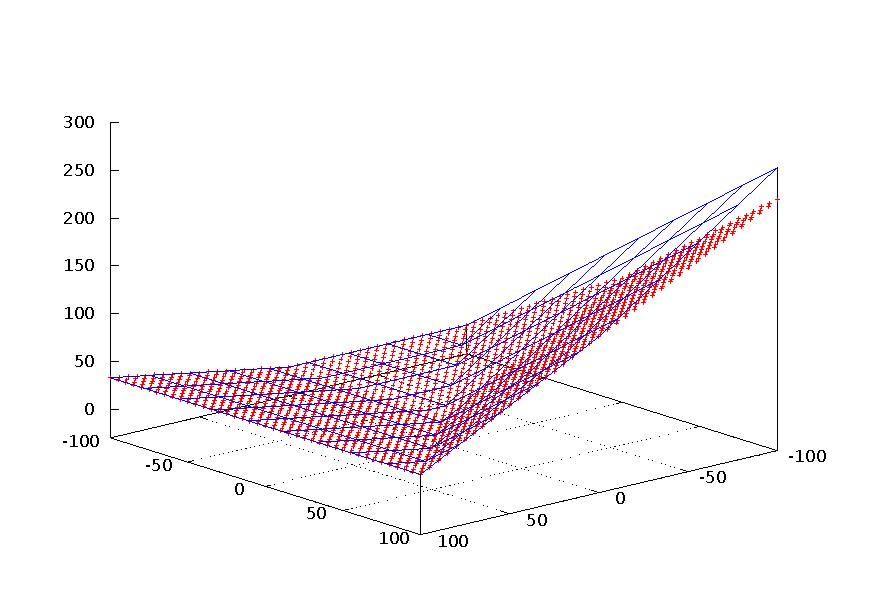
\includegraphics[width=.9\linewidth]{fig/bound3d}
\caption{The automatically derived bound $1.33|[x,y]| + 0.33 |[0,x]|$
  (blue lines) and the measured runtime cost (red crosses) for Example
  \emph{t08}. For $x\ge 0$ the bound is tight.}
\label{fig:3d}
\end{figure}


\sectskip
\section{Related Work}
\label{sec:related}
\aftersectskip

Our work has been inspired by type-based amortized resource analysis
for functional programs~\cite{Jost03,HoffmannH10,HoffmannAH12}.  Here,
we present the first automatic amortized resource analysis for
C. None of the existing techniques can handle the example programs we
describe in this work.
%
The automatic analysis of realistic C programs is enabled by two
major improvements over previous work.  First, we extended the
analysis system to associate potential with not just individual
program variables but also multivariate intervals
and, more generally, auxiliary variables.  In this way, we solved the
long-standing open problem of extending automatic amortized resource
analysis to compute bounds for programs that loop on (possibly
negative) integers without decreasing one individual number in each
iteration.  Second, for the first time, we have combined an automatic
amortized analysis with a system for interactively deriving bounds. In
particular, recent systems~\cite{HoffmannS13} that deal with integers
and arrays cannot derive bounds that depend on values in mutable
locations, possibly negative integers, or on differences between
integers.

A recent project~\cite{veristack14} has implemented and verified a
quantitative logic to reason about stack-space usage, and modified the
verified CompCert C compiler to translate C level bound to x86 stack
bounds.  This quantitative logic is also based on the potential method
but has very rudimentary support for automation. It is not based on
efficient LP solving and cannot automatically derive symbolic
bounds.  In contrast, our main contribution is an automatic amortized
analysis for C that can derive parametric bounds for loops and
recursive functions fully automatically.
%
In this article, we also use a more general quantitative Hoare
logic that is parametric in the resource of interest.

\iffull{
In the development of our quantitative Hoare logic we have drawn
inspiration from mechanically verified Hoare logics.
Nipkow's~\cite{Nipkow02} description of his implementations of Hoare
logics in Isabelle/HOL has been helpful to understand the interaction
of auxiliary variables with the consequence rule.  Appel's separation
logic for CompCert Clight~\cite{AppelLogic} has been a blueprint for
the general structure of the quantitative logic.  \iffull{Since we do not deal
with memory safety, our logic is much simpler and it would be possible
to integrate it with Appel's logic.}{}  The continuation passing style
that we use in the quantitative logic is not only used by
Appel~\cite{AppelLogic} but also in Hoare logics for low-level
code~\cite{NiS06,JensenBK13}.

There exist quantitative logics that are integrated into separation
logic~\cite{Atkey10,HoffmannMZ13} and they are closely related to our
quantitative logic.  However, the purpose of these logics is slightly
different since they focus on the verification of bounds that depend
on the shape of heap data structures and they are not implemented for
C.  Also closely related to our logic is a VDM-style logic for
reasoning about resource usage of an abstract fragment of JVM byte
code by Aspinall et al.~\cite{AspinallBHLM07}.  Their logic is not
Hoare-style, does not target C code, and is not designed for
interactive bound development but to produce certificates for bounds
derived for high-level functional programs.
}{}

There exist many tools that can automatically derive loop and
recursion bounds for imperative programs such as
SPEED~\cite{GulwaniMC09,GulwaniZ10}, KoAT~\cite{BrockschmidtEFFG14},
PUBS~\cite{AlbertAGPZ12}, Rank~\cite{AliasDFG10},
ABC~\cite{BlancHHK10} and LOOPUS~\cite{Zuleger11,SinnZV14}.  These
tools are based on abstract interpretation--based invariant generation
and/or term rewriting techniques, and they derive impressive results
on realistic software.  The importance of amortization to derive tight
bounds is well known in the resource analysis
community~\cite{AlonsoG12,Moser14,SinnZV14}.  Currently, the only
other available tools that can be directly applied to C code are Rank
and LOOPUS.  As demonstrated, $\toolname$ is more compositional than
the aforementioned tools. Our technique, is the only one that is able
to generate resource specifications for functions, deal with resources
like memory that might become available, generates proof certificates
for the bounds, and has support for user guidance that separates
qualitative and quantitative reasoning.

There are techniques~\cite{Braberman08} that can compute the memory
requirements of object oriented programs with region-based garbage
collection.  \iffull{These systems infer invariants and use external tools
that count the number of integer points in the corresponding polytopes
to obtain bonds.  The described technique can handle loops but not
recursive or composed functions.}{ These systems can handle loops but not
recursive or composed functions.}
%
We are only aware of two verified quantitative analysis systems.
Albert et al.~\cite{AlbertBGHR12} rely on the KeY tool to
automatically verify previously inferred loop invariants, size
relations, and ranking functions for Java Card programs.  However,
they do not have a formal cost semantics and do not prove the bounds
correct with respect to a cost model.  Blazy et al.~\cite{Blazy13}
have verified a loop bound analysis for CompCert's RTL intermediate
language.  However, this automatic bound analysis does not
compute symbolic bounds. \iffull{Furthermore, there is no way to
  interactively derive bounds or to deal with resources like memory
  usage.}



\sectskip
\section{Conclusion}
\label{sec:concl}
\aftersectskip

We have developed a novel analysis framework for compositional and
certified worst-case resource bound analysis for C programs.  The
framework combines ideas from existing abstract interpretation--based
techniques with the potential method of amortized analysis.  It is implemented in the publicly available tool
$\toolname$. To the best of our knowledge, $\toolname$ is the first
analysis tool for C programs that automatically reduces the derivation
of symbolic bounds to LP solving.

We have demonstrated that our approach improves the state-of-the-art
in resource bound analysis for C programs in three ways. First, our
technique is naturally compositional, tracks size changes of
variables, and can abstractly specify the resource cost of functions
(\pref{sec:AAA}). Second, it is easily combinable with established
qualitative verification to guide semi-automatic bound derivation
(\pref{sec:anno}). Third, we have shown that the local inference rules
of the derivation system automatically produce easily checkable
certificates for the derived bounds (\pref{sec:soundness}).
%
Our system is the first amortized resource analysis for C programs.
It addresses the long-standing open problem of extending automatic
amortized resource analysis to compute bounds for programs that loop
on signed integers and to deal with non-linear control flow\ifshort{.}{ that is
introduced by break and return statements.}

This work is the starting point for several projects that we plan to
investigate in the future, such as the extension to
concurrency, better integration of low-level features like
memory caches, and the extension of the automatic analysis to
multivariate resource polynomials~\cite{HoffmannAH11}.

% \acks

% This research is based on work supported in part by NSF grants 1319671
% and 1065451, and DARPA grants FA8750-10-2-0254 and FA8750-12-2-0293.
% Any opinions, findings, and conclusions contained in this document are
% those of the authors and do not reflect the views of these agencies.



\ifx\fullversion\undefined{}\else{
%\clearpage
\appendix

\newpage

\section{Syntax and Semantics}
\label{app:sem}

We implemented our cost semantics and the quantitative Hoare logic in
Coq for \emph{CompCert Clight}.  Clight is the most abstract
intermediate language used by CompCert.  Mainly, it is a subset of C
in which loops can only be exited with a \code{break} statement and
expressions are free of side effects.

\paragraph{Syntax.}

In this article, we describe our system for a subset of Clight that is
sufficient to discuss the general ideas.  This subset is given by the
following grammar.
%
\begin{align*}
S &:= \code{assert}~E
\mid \code{skip}
\mid \code{break}
\mid \code{return}~x
\mid x \gets E
\mid x \gets f(x^*)
\\
& \mid \code{loop}~S
\mid \code{if}(E)~S~\code{else}~S
\mid S;S
\mid \code{tick}(n)
\end{align*}
%
Expressions $E$ are left abstract in our presentation.  For our
analysis framework, it is only important that they are side-effect
free.
%
The most notable difference to full Clight is that we can only assign
to variables and thus do not consider operations that update the heap.
Moreover, function arguments and return values are assumed to be
variables.  This is only for simplifying the presentation; in the
implementation we can deal with heap updates and general function
calls and returns.  However, we have not implemented our framework for function
pointers, \code{goto} statements, \code{continue} statements, and
\code{switch} statements.

We include the built-in primitive $\code{assert}~e$ that terminates
the program if the argument $e$ evaluates to false and has no effect
otherwise.  This is useful to express assumptions on the inputs of a
program for the automatic analysis.  We also add the built-in function
\code{tick(n)} that can be called with a constant integer $n$ as a
flexible way to model resource consumption or release (if $n$ is
negative).


\begin{figure*}[t!]
\begin{mathpar}
%
\Rule{S:Assert}
{ \code{istrue}~\sem{e}_\state }
{ (\state, \code{assert}~e, \cont, \cost)
\smallstep{M}
(\state, \code{skip}, \cont, \cost {-} M_a)
}
%
\and
\Rule{S:BrkSeq}
{}
{ (\state, \code{break}, \Kseq S \cont, \cost)
\smallstep{M}
(\state, \code{break}, \cont, \cost)
}
%
\and
\Rule{S:BrkLoop}
{}
{ (\state, \code{break}, \Kloop S \cont, \cost)
\smallstep{M}
(\state, \code{skip}, \cont, \cost {-} M_b)
}
%
\and
\Rule{S:RetSeq}
{}
{ (\state, \code{return}~x, \Kseq S \cont, \cost)
\smallstep{M}
(\state, \code{return}~x, \cont, \cost)
}
\and
%
\and
\Rule{S:RetLoop}
{}
{ (\state, \code{return}~x, \Kloop S \cont, \cost)
\smallstep{M}
(\state, \code{return}~x, \cont, \cost)
}
%
\and
\Rule{S:RetCall}
{ \state = (\_, \gamma) \\
  \state' = (\theta, \gamma)[r \mapsto \state(x)]
}
{ (\state, \code{return}~x, \Kcall r \theta \cont, \cost)
\smallstep{M}
(\state', \code{skip}, \cont, \cost {-} M_r)
}
%
\and
\Rule{S:Update}
{ \state' = \state[x \mapsto \sem{e}_\state] }
{ (\state, x \gets e, \cont, \cost)
\smallstep{M}
(\state', \code{skip}, \cont, \cost {-} M_u {-} M_e(e))
}
%
\and
\Rule{S:Call}
{ \fenv f = (\vec x, S_f) \\
  \state = (\theta, \gamma) \\
  \state' = (\vec x \mapsto \state(\vec y), \gamma) \\
}
{ (\state, r \gets f(\vec y), \cont, \cost)
\smallstep{M}
(\state', S_f, \Kcall r \theta \cont, \cost {-} M_f)
}
%
\and
\Rule{S:Loop}
{}
{ (\state, \code{loop}~S, \cont, \cost)
\smallstep{M}
(\state, S, \Kloop S \cont, \cost)
}
%
\and
\Rule{S:SkipLoop}
{}
{ (\state, \code{skip}, \Kloop S \cont, \cost)
\smallstep{M}
(\state, \code{loop}~S, \cont, \cost {-} M_l)
}
%
\and
\Rule{S:IfTrue}
{ \code{istrue}~\sem{e}_\sigma
\\ \cost' = \cost {-} M_c^1 {-} M_e(e)
}
{ (\state, \code{if}(e)~S_1~\code{else}~S_2, \cont, \cost)
\smallstep{M}
(\state, S_1, \cont, \cost')
}
%
\and
\Rule{S:IfFalse}
{ \code{isfalse}~\sem{e}_\sigma
\\ \cost' = \cost {-} M_c^2 {-} M_e(e)
}
{ (\state, \code{if}(e)~S_1~\code{else}~S_2, \cont, \cost)
\smallstep{M}
(\state, S_2, \cont, \cost')
}
%
\and
\Rule{S:Seq}
{ }
{ (\state, S_1; S_2, \cont, \cost)
\smallstep{M}
(\state, S_1, \Kseq {S_2} \cont, \cost)
}
%
\and
\Rule{S:SkipSeq}
{}
{ (\state, \code{skip}, \Kseq S \cont, \cost)
\smallstep{M}
(\state, S, \cont, \cost {-} M_s)
}
%
\and
\Rule{S:Tick}
{ }
{ (\state, \code{tick}(n), \cont, \cost)
\smallstep{M}
(\state, \code{skip}, \cont, \cost {-} M_t(n))
}

\end{mathpar}
\caption{Rules of the operational semantics of statements.}
\label{fig:opsem}
\end{figure*}




\section{Quantitative Hoare Logic}
\label{app:logic}

\begin{figure*}
\begin{mathpar}
%
\Rule{L:Skip}
{ }
{ \Delta; B; R \vdash
\htriple
  { Q }{ \code{skip} }{ Q }
}
%
\and
\Rule{L:Break}
{ }
{ \Delta; B; R \vdash
\htriple
  { M_b + B }{ \code{break} }{ Q }
}
%
\and
\Rule{L:Return}
{ }
{ \Delta; B; R \vdash
\htriple
  { R\,(\state(x)) }{ \code{return}~x }{ Q }
}
%
\and
\Rule[leftskip=.0cm,rightskip=.0cm]{L:Update}
{ }
{ \Delta; B; R \vdash
\htriple
  { \lambda \state.\,M_u + M_e(e) + Q\,\state[x \mapsto \sem{e}_\state] }{ x \gets e }{ Q }
}
%
\and
\Rule[leftskip=.0cm,rightskip=.0cm]{L:Seq}
{ \Delta; B; R \vdash
\htriple{ P }{ S_1 }{ Q' + M_s }
\\
\!\!  \Delta; B; R \vdash
\htriple{ Q' }{ S_2 }{ Q }
}
{ \Delta; B; R \vdash
\htriple{ P }{ S_1;S_2 }{ Q }
}
%
\and
\Rule{L:Call}
{
  \Delta(f) = \forall z\,\vec v\,v.(P_f\,z\,\vec v, Q_f\,z\,v) \\
  P \models P_f \, y \, (\state(\vec x)) \land A \\
  \forall v.\, (Q_f \, y \, v \land A \models \lambda \state.\, Q \, \state[r \mapsto v])
}
{ \Delta; B; R \vdash
\htriple
  { M_f + P }
  { r \gets f(\vec x) }
  { Q - M_r }
}
%
\and
\Rule{L:Assert}
{ }
{ \Delta; B; R \vdash
\htriple
  { \code{istrue}~\sem{e}_\state \implies Q + M_a }
  { \code{assert}~e }
  { Q }
}
%
\and
\Rule{L:Tick}
{ }
{ \Delta; B; R \vdash
\htriple
  { Q + M_t(n) }
  { \code{tick}(n) }
  { Q }
}
%
\and
\Rule{L:Loop}
{ \Delta; Q; R \vdash
\htriple
  { I }{ S }{ I + M_l }
}
{ \Delta; B; R \vdash
\htriple
  { I }{ \code{loop}~S }{ Q }
}
%
\and
\Rule{L:If}
{ \Delta; B; R \vdash
\htriple
  { \code{istrue}~\sem{e}_\state + P - M_c^1}
  { S_1 }{ Q }
\\
  \Delta; B; R \vdash
\htriple
  { \code{isfalse}~\sem{e}_\state + P - M_c^2 }
  { S_2 }{ Q }
}
{ \Delta; B; R \vdash
\htriple
  { P + M_e(e) }{ \code{if}(e)~S_1~\code{else}~S_2 }{ Q }
}
%
\and
\Rule{L:Weaken}
{
  \!\! P \models P' \!\! \\
  \!\! \Delta; B'; R' \vdash
  \htriple{ P' }{ S }{ Q' } \!\! \\
  \!\! Q' \models Q \!\! \\
  \!\! B' \models B \!\! \\
  \!\! \forall v.\, (R'\,v \models R\,v) \!\!
}
{ \Delta; B; R \vdash
\htriple{ P }{ S }{ Q }
}
%
\and
\Rule{L:Frame}
{ \Delta; B; R \vdash
\htriple{ P }{ S }{ Q } \\
  x \in \Qplusz
}
{ \!\! \Delta; B + x; R + x \vdash
\htriple{ P + x }{ S }{ Q + x } \!\!
}
%
\and
\Rule{L:Extend}
{ \Delta \cup \Delta'; B; R \vdash
  \htriple{ P }{ S }{ Q }
\\
  \forall f\,P_f\,Q_f.\,
  \Delta'(f) = \forall z\,\vec v\,v.(P_f\,z\,\vec v, Q_f\,z\,v)
  \rightarrow
  \forall y\,\vec v.\,
  (\Delta \cup \Delta'; \bot; Q_f\,y \vdash
    \htriple{ P_f\,y\,\vec v }{ S_f }{ \bot })
}
{ \Delta; B; R \vdash
\htriple{ P }{ S }{ Q }
}
%
\end{mathpar}

\caption{Rules of the Quantitative Hoare Logic}
\label{fig:logicapp}
\end{figure*}

In this section we describe a simplified version of the quantitative
Hoare logic that we use in Coq to interactively prove resource bounds.
%
We generalize classic Hoare logic to express not only classical
boolean-valued assertions but also assertions that talk about the
future resource usage.  Instead of the usual assertions $P : \State
\to \mathit{bool}$ of Hoare logic we use assertions
$$
P : \State \to \Qplusz \cup \{ \infty \} \; .
$$
This can be understood as a refinement of boolean assertions where
$\mathit{false}$ is $\infty$ and $\mathit{true}$ is refined by $\Qplusz$.
We write $\Assn$ for $\State \to \Qplusz \cup \{ \infty \}$ and $\bot$ for
$\lambda \state . \, \infty$.  We sometimes call assertions
\emph{potential functions}.  To use Coq's support for propositional
reasoning, assertions have the type $\State \to \Qplusz \to \mathrm{Prop}$
in the implementation.  For a given $\state \in \State$, such an
assertion can be seen as a set $B \subseteq \Qplusz$ of valid bounds.
However, we find the presentation in this article easier to read.

Due to \code{break} and \code{return} statements of Clight, there are
different possible ways to exit a block of code.  We also have to keep
track of the resource specifications of functions.  To account for
this in the logic, our quantitative Hoare triples have the form
$$
\Delta; B; R \vdash
\htriple
  { Q }
  { S }
  { Q' } \; .
$$
The triple $\htriple{ Q }{ S }{ Q' }$ consists of a statement $S$ and
two assertions $Q,Q' : \Assn$.  It corresponds to triples in classic
Hoare logic and the intuitive meaning is as follows.  If $S$ is
executed with starting state $\state$, the empty continuation
$\Kstop$, and at least $P(\state)$ resources available then the
evaluation does not run out of resources and there are at least
$Q(\state')$ resources left if the evaluation terminates in state
$\state'$.  The assertion $B : \Assn$ provides the
postcondition for the case in which the code block $S$ is exited by a
\code{break} statement.  So if the execution is terminated in state
$\state'$ with a \code{break} then $B(\state')$ resources are
available.  Similarly, $R : \Z \to \Assn$ is the postcondition for the
case in which the code block $S$ is exited by a $\code{return}~x$
statement.  The integer argument of $R$ is the return value.
Finally, the function context of judgements that we write $\Delta$ is
a mapping from function names to specifications of the form
$$
  \forall z \, \vec v \, v .(P_f \, z \, \vec v, Q_f \, z \, v).
$$
The assertion $P_f \, z \, \vec v$ is the precondition of the function
$f$ and the assertion $Q_f \, z \, v$ is its postcondition.  They are
both parameterized by an arbitrary logical variable $z$ (which can be a
tuple) that relates the function arguments with the return value.  The
precondition also depends on $\vec v$, the values of the arguments
at the function invocation.  Similarly, the postcondition depends on
the return value $v$ of the function.  The use of logical variables to
express relations between different states of an execution is a
standard technique of Hoare logic.
%
To ensure soundness, we require that $P_f$ and $Q_f$ do not depend on
the local variables on the stack, that is, $\forall z \, \vec v
\, \theta \, \theta' \, \gamma . \, P_f \, z \, \vec v \,
(\theta,\gamma) = P_f \, z \, \vec v \, (\theta',\gamma)$.

For two assertions $P,Q : \Assn$, we write $P \models Q$ to if for all
program state $\state$ $P(\state) \ge Q(\state)$.

\paragraph{Rules of the Quantitative Logic.}

\pref{fig:logicapp} shows the inference rules of the quantitative logic.
The rules are slightly simplified in comparison to the implemented
rules in Coq.  The main difference is that the presented version does
not formalize the heap operations.

In the rule {\sc L:Skip}, we do not have to account for any resource
consumption.  As a result, the precondition $Q$ can be any (potential)
function and we only have to make sure that we do not end up with more
potential.  Since the execution of \code{skip} leaves the program
state unchanged, we can simply use the precondition as postcondition.
The potential functions $B$ for the \code{break} and $R$ for the
\code{return} part of the postcondition are not reachable and can
therefore be arbitrary.

In the rule {\sc L:Assert}, we use the notation
$\code{istrue}~\sem{e}_\state \implies Q + M_a$ to express that we
require potential $Q + M_a$ in the precondition if $e$ evaluates to
$\mathit{true}$ in the current program state.  If $e$ evaluates to
$\mathit{false}$ then the potential in the precondition can be
arbitrary since the program will be terminated.

In the rules {\sc L:Break} and {\sc L:Return}, the postcondition can
be arbitrary since it is unreachable.  Instead, we have to justify the
potential functions $B$ and $R$ that hold after a \code{return} and a
\code{break}, respectively.  In {\sc L:Break}, we require to have
potential $M_b+B$ in the precondition: $M_b$ to pay for the execution
cost of \code{break} and $B$ to pay for the potential after the
\code{break}.  In {\sc L:Return} we only require to have potential
$R$ in the precondition to pay for the potential after the
\code{return}.  The reason is that we found it to be more convenient
to account for the execution cost $M_r$ of the return in rule {\sc
  L:Call} for function calls.

The rule {\sc L:Update} is the standard assignment rule of Hoare
logic.  With the substitution $\state[x \mapsto \sem{e}_\state]$ in
the precondition we ensure that $Q$ evaluates to the same number as in
the postcondition.  We also require that have we the constant
potential $M_u + M_e(e)$ available in the precondition to pay for the
cost of the evaluation of $e$ and the update.

The rule {\sc L:Seq} rule is crucial to understand how the
quantitative Hoare logic works.  To account for early exits of
statements, we must ensure in the \code{break} part $B$ of $S_1$'s
judgement that the \code{break} part $B$ of of $S_1;S_2$ holds. The
same is true for the return part $R$ of the judgements for $S_1$ and
$S_2$.  The interaction between the actual pre- and postconditions is
analogous to standard Hoare logic.  In the postcondition of $S_1$ we
account for the cost $M_s$ of the execution of the sequence.

In the rule {\sc L:Loop}, the \code{break} part of the
loop body $S$ becomes the postcondition of the loop statement. We use
an arbitrary $B$ as the \code{break} part of the judgement for
$\code{loop}\, S$ since its operational semantics ensures that it can
only terminate with a \code{skip} or a \code{return}.  The
precondition $I$ of the loop is the loop invariant.  That is why we
require to have potential $I$ available in the precondition of the
loop body $S$.  In the postcondition of $S$, the potential must be
sufficient to pay for the invariant $I$ and the cost $M_l$ of the loop
iteration.

The {\sc L:If} is similar to the rule for the conditional in classic
Hoare logic.  In the preconditions of the judgments for the two
branches $S_1$ and $S_2$ we lift the boolean assertions
$\code{isfalse}~\sem{e}_\state$ and $\code{isfalse}~\sem{e}_\state$ to
quantitative assertions.  In the precondition of the rule {\sc L:Tick}
we account for the execution cost $M_t(n)$ of the \code{tick}
statement that depends on the integer $n$.

The rule {\sc L:Call} accounts for the execution cost of both $M_f$
for function calls and $M_r$ for \code{return} statements.
This justifies that the {\sc L:Return} rule does not account
  for resource consumption. The pre- and postcondition $P_f$ and
$Q_f$ are taken from the function context $\Delta$.  The assertions in
the context are parametric with respect to both the values of the
function arguments and the return value. This allows us to specify a
bound for a function whose resource consumption depends on its
arguments.  The arguments are instantiated by the call rule
using the result of the evaluation of the argument variables in the
current state.  Recall that we require that $P_f$ and $Q_f$ do
  not depend on the local variables on the call stack, that is,
  $\forall z \, \vec v \, \theta \, \theta' \, \gamma . \, P_f \, z \,
  \vec v \, (\theta,\gamma) = P_f \, z \, \vec v \,
  (\theta',\gamma)$. To transfer potential that depends on local
variables of the callee from the precondition $P$ to the postcondition
$Q$, we use an assertion $A : \Assn$ that is independent of global
variables, that is, $\forall \theta \, \gamma \, \gamma' . \, A
(\theta,\gamma) = A(\theta,\gamma')$.  It is still possible to express
relations between global and local variables using logical
variables (see the following paragraph for details).

Finally, we describe the rules which are not syntax directed.  There
are two weakening rules available in the quantitative Hoare logic.
The framing rule {\sc L:Frame} is designed to weaken a statement by
stating that if $S$ needs $P$ resources to run and leaves $Q$
resources available after its execution, then it can very well run
with $P + c$ resources and return $Q + c$ resources.  The consequence
{\sc L:Conseq} rule is directly imported from classical Hoare logic
except that instead of using the logical implication $\Rightarrow$ we
use the quantitative $\models$ that point-wise applies $\ge$.  This
rule indeed weakens the statement since it requires more resource to
run the statement and yields less than what has been proved to be
available after its termination.

\paragraph{Logical Variables and Shallow Embedding.}

When specifying a program, it is often necessary to relate certain
invariants in the pre- and postcondition.  A standard solution of Hoare
logic is to use \emph{logical variables}~\cite{Kleymann99}.  These
additional variables (also called auxiliary state in the literature)
are constant across the derivation.  For example, if $Z$ is such
a logical variable, we can specify the function $\code{double}()$
which doubles the global variable $x$ as
$$
  \htriple{z = Z}{\code{double}()}{x = 2 \cdot Z}.
$$
%
When formalizing Hoare logics in a proof assistant one can either
fully specify the syntax and semantics of assertions and hence get a
deep embedding, or use the assertions of the host theory to get a
shallow embedding.  Because of its flexibility, we used the latter
approach in our development.  This choice makes it possible to have
logical variables almost for free: we can simply use the variable and
binding mechanisms of Coq, our host theory.  When an logical variable
is needed we introduce it using a universal quantifier of Coq before
using the logic to derive triples.  For example, the Coq theorem for
the above example would look as follows.
%
\begin{lstlisting}
Theorem dbl_triple: forall Z,
  qtriple ($\lambda\sigma$.$\sigma$(x) = Z) ($\code{double}()$) ($\lambda\sigma$.$\sigma$(x) = 2*Z).
\end{lstlisting}
%
However, this trick alone is often not sufficient when working with a
recursive function $f$.  In that case we apply the {\sc L:Extend} rule
of the logic.  First we add a specification $\forall z\,\vec
v\,v.(P_f\,z\,\vec v, Q_f\,z\,v)$ of $f$ to the function context
$\Delta$.  Then we proceed to prove the function body $S_f$ with this
induction hypothesis.  In this process it can be the case that we have
to use the induction hypothesis with a different value of a logical
variable (e.g., because the values of the arguments in the recursive
call differ from the values of the arguments of the callee).  To cope
with this problem, assumptions in the function context $\Delta$ are
universally quantified over logical variables.  The {\sc L:Extend}
rule uses the host proof assistant to require that the triple on $f$'s
body is proved for every possible logical variable $y$.

\paragraph{Using the Quantitative Logic.}

In the following we demonstrate the use of the logic with two example
derivations.

In the example in~\pref{fig:xmplmax} we derive a precise runtime
bound on a program that searches a maximal element in an array.  The
cost metric that we use simply counts the assignments performed by the
program.  Hence, the resource cost is closely related to the
number of times the test \code{a[i] > m} is true during the
execution.
%
If we define
$$
 A(i) =  \# \{ k \mid i \le k < N \land \forall\, 0 \le j < k.\, a[j] < a[k] \} \, .
$$
where we write $\# S$ for the cardinal of the set $S$ then $A(1)+1$ is
the number of ``maximum candidates'' in the array \code{a} seen
by the algorithm. $A(1)$ is bounded by $N$, the size of the array.
So any automated tool would at best derive the linear bound $2 \cdot
N$ for that program.  But with the expressivity of our logic it is
possible to use the previous set cardinal directly and precisely tie
the bound to the initial contents of the array.
%
The non-trivial part of this derivation is finding the loop invariant
$(m = \max_{k \in [0, i-1]} a[k]) + A(i) + (N-i)$ for the while loop.
When the condition \code{a[i] > m} is true, we know that we
encountered a ``maximum so far'' because $m$ is a maximal element of
\code{a[0 \dots i]}, thus $A(i) = 1 + A(i+1)$ and we get one
potential unit to pay for the assignment.  In the other case, no
maximum so far is encountered so $A(i) = A(i+1)$.
% As a side remark, if $K \ge 0$, it is possible to
% have $\{ A(0) + N + K \}$ and $\{ K \}$ as pre- and postcondition
% of the same program.  It can be done either by adapting the proof or by
% applying the {\sc L:Frame} rule one top of the triple already derived.
% More generally, without function calls, the {\sc L:Frame}
% rule is admissible in our system.

The example in~\pref{fig:xmplbs} shows a use case for logical
variables as well as a metric for stack consumption. In a stack
metric, we account a constant cost for a function call ($M_f>0$) that
is returned after the call ($M_r = -M_f <0$).  All other resource cost
are $0$.  We are interested in showing that a binary search function
$\code{bsearch}$ has logarithmic stack consumption.  We use a logical
variable $Z$ in the function specification $\htriple{(Z = \log_2(h-l))
  + Z \cdot M_\code{bsearch}}{}{Z \cdot M_\code{bsearch}}$ to express that the stack required by the
function is returned after the call.
%
The critical step in the proof is the application of the
{\sc L:Call} rule to the recursive call.  At this point
the context $\Delta$ contains the specification
$
  \forall y \, (x,l,h) \, \_.
  ( (\lambda y \, (\_, l, h) .\, (y = \log_2(h {-} l)) {+} y {\cdot} M_\code{bsearch})
  , (\lambda y \, \_ .\, y {\cdot} M_\code{bsearch})
  )
$.
%
Using the rule {\sc L:Call} it is possible to instantiate $y$ with $Z
- 1$, and because $M_f = M_\code{bsearch}$ and $M_r =
-M_\code{bsearch}$ in the stack metric.  The rest of the proof does
not involve any resource manipulation and is just bookkeeping of
logical assertions.



\begin{figure}
\begin{lstlisting}
${\color{blue} \{ A(0) + N \} }$
i=1; m=a[0];
${\color{blue}%
  \{ (i {=} 1 \land m=a[0]) + A(1) + (N-1) \} }$
while (i < N) {
  ${\color{blue}%
    \{ (m = \max_{k \in [0, i-1]} a[k]) + A(i) + (N-i) \} }$
  if (a[i] > m)
    m=a[i];
  ${\color{blue}%
    \{ (m = \max_{k \in [0, i]} a[k]) + A(i+1) + (N-i) \} }$
  i=i+1;
  ${\color{blue}%
    \{ (m = \max_{k \in [0, i-1]} a[k]) + A(i) + (N-i) \} }$
} ${\color{blue} \{ 0 \} }$
\end{lstlisting}
\caption{Example derivation where we wrote $A(i)$
  for $\#\{ k \mid i \le k \le N \land \forall\, 0\le j<k.\, a[j] < a[k]\}$,
  the metric used here assigns a cost of 1 to every assignment
  and 0 to all other operations.
  }
\label{fig:xmplmax}
\end{figure}

\begin{figure}
\begin{lstlisting}
${\color{blue}%
  \{ (Z = \log_2(h-l)) + Z \cdot M_\code{bsearch} \} }$
bsearch(x,l,h) {
  if (h-l > 1) {
    ${\color{blue}%
      \{ (Z \ge 1 \land Z = \log_2(h-l)) + Z \cdot M_\code{bsearch} \} }$
    m = h + (h-l)/2;
    ${\color{blue}%
      \{ (m = \frac{h+l}{2} \land Z \ge 1 \land Z = \log_2(h-l)) + Z \cdot M_\code{bsearch} \} }$
    if (a[m]>x) h=m; else l=m;
    ${\color{blue}%
      \{ (Z - 1 = \log_2(h-l)) + (Z-1) \cdot M_\code{bsearch} + M_\code{bsearch} \} }$
    l = bsearch(x,l,h); }
  ${\color{blue}%
    \{ (Z-1) \cdot M_\code{bsearch} - (-M_\code{bsearch}) \} }$
  return l;
} ${\color{blue} \{ Z \cdot M_\code{bsearch} \} }$
\end{lstlisting}
\caption{Example derivation of a stack usage bound for a binary
  search program.  The used resource metric defines the cost $M_\code{bsearch}$ before
  the function call and $-M_\code{bsearch}$ after the call.  $M_\code{bsearch}$ is the stack
  frame size of the function $\code{bsearch}$.  $Z$ is a
  logical variable.
  }
\label{fig:xmplbs}
\end{figure}


\paragraph{Soundness of Quantitative Hoare Triples.}

We already gave an intuition of the meaning of judgements
derived in the logic.  To make it formal, we define the
\emph{resource safety} $\safe n P S \cont$ of an assertion
and a program configuration as $\forall \state \, \cost \, m \, \cost' .$
\begin{align*}
  (m {\le} n \land P(\state) {\le} \cost \land
    (\state, S, \cont, \cost) \smallstep{M}^m (\_, \_, \_, \cost'))
  \implies \cost' {\ge} 0.
\end{align*}
This predicate is step indexed by an integer $n$ that is used for
induction in the soundness proof for the function-call and loop cases.
The constraint $\cost' \geq 0$ imposed by the definition ensures that
the program does not stop because of a resource error (recall that a
negative resource counter on the right-hand side is a resource
failure).  However, it does not rule out memory safety errors or
assertion failures. This is because our logic does not prove any
safety or correctness theorems but only focuses on resource usage.
%
An interesting detail in the definition is the natural number $m$.  We
simply use it to ensure that $\safe {n+1} P S \cont \implies \safe n P S
\cont $.  This would not be the case if we replaced all occurrences of
$m$ by $n$ in the definition of validity.

The resource safety of a continuation $\cont$ is defined using three
assertions, one for each of the possible outcomes of a program
statement.  We define it as follows.
\begin{align*}
\safeK n B R Q \cont & :=  \safe n B {\code{break}} \cont \\
 \land& \safe n {\lambda \state.\,R\,(\state(x))} {\code{return}~x} \cont \\
 \land& \safe n Q {\code{skip}} \cont
\end{align*}
%
We can now define the \emph{semantic validity} of a judgement $B; R
\vdash \htriple P S Q$ of the quantitative logic without function
context as $\valid n B R P S Q :=$
\begin{align*}
& \forall m \, \cont \, x \geq 0 .\, (m \le n \land \safeK m {B{+}M_b{+}x} {R{+}x} {Q{+}x} \cont) \\
& \implies \safe m {P+x} S \cont \; .
\end{align*}
Note how the validity of a triple embeds the frame rule of
our logic. This refinement is necessary to have a stronger
induction hypothesis available during the proof.
%
We again need to add the auxiliary $m$ to ensure that $\valid {n{+}1} B R P
S Q$ implies $\valid n B R P S Q$.

Using the semantic validity of triples we define the validity
of a function context $\Delta$, written $\validC n \Delta$, as
\begin{align*}
  &\forall f .\, \Delta(f) =
    \forall z \, \vec v \, v .(P_f \, z \, \vec v, Q_f \, z \, v)
    \implies \\
  &\qquad \forall z \, \vec v .\,
  \valid n \bot {Q_f \, z} {P_f \, z \, \vec v} {S_f} \bot ,
\end{align*}
where $S_f$ is the body of the function $f$. A full
judgement that mentions a non-empty function context
$\Delta$ is in fact a guarded statement: it makes
assumptions on some functions' behavior.  The predicate
$\validC n \Delta$ gives the precise meaning of the
assumptions made.  It is also step-indexed to prove the
soundness of the {\sc L:Extend} rule by induction.
%
We are now able to state the soundness of the quantitative logic.
%
\begin{theorem}[Soundness]
  If $\Delta; B; R \vdash \htriple P S Q$ is derivable then
  $
    \forall n .\, \validC n \Delta
      \implies \valid {n {+} 1} B R P S Q.
  $
\end{theorem}
%
\noindent
The difference $\delta = 1$ between the index in the triple
validity and the one in context validity arises from
the soundness proofs of {\sc L:Call} and {\sc L:Extend}.  For
{\sc L:Call}, the language semantics makes one step and
proceeds with the function body, so we must have
$\delta \le 1$ to use the assumptions in $\Delta$.
For {\sc L:Extend}, we have to show that $\Delta \cup \Delta'$
is a valid context for $n$ steps.  The induction hypothesis
in that case says that if $\Delta \cup \Delta'$ is valid
for $m$ steps, $\Delta'$ is valid for $m+\delta$ steps.
So if we want to solve this goal by induction, it is
necessary that $\delta \ge 1$.  These two constraints force
$\delta$ to be exactly one in the theorem statement.

Assume that $S$ is a complete program and $\Delta$ is empty.  By
expanding the definitions we see that $\Delta$ is valid
for every $n$ and that $\Kstop$ is safe for every $n$. So
we derive
$$
\Delta; B; R \vdash \htriple P S Q \implies   \forall n .\, \safe n P S \Kstop.
$$
This means that from any starting state $\state$, $P(\state)$
provides enough resources for any run of the program $S$.  This
setting is actually the main use case of the previous theorem
which is stated as a stronger result to allow a proof by
induction.




\section{Catalog of Automatically Analyzed Programs}
\label{app:cat}

In this appendix we provide a non-exhaustive catalog of classes of
programs that can be automatically analyzed by our system.  For
simplicity, and to compare our analysis with existing tools, we use a
cost metric that counts the number of loop iterations and function
calls.  This is the only cost metric supported by tools like
KoAT~\cite{BrockschmidtEFFG14} and LOOPUS~\cite{SinnZV14}.  Sometimes
we also use the \emph{tick metric} if we want to discuss features such as
resource restitution.  The tick metric assigns cost $n$ to the
statement \code{tick(n)} and cost $0$ to all other statements. Of
course, the examples can also be analyzed with any other cost metric
in our system.

We assume that free variables in the code snippets are the inputs of
the program. Some of the examples contain constants on which the
computed bound depends.  These constants are randomly chosen to
present an example but the analysis works for other constants as well.
Note however that it is sometimes crucial that constants are positive
(or negative) or that other relations hold.

\pref{tab:eval} contains the details of our comparative evaluation.


\begin{figure*}
\setlength{\progwidth}{.24\linewidth}
  \centering

  \begin{minipage}[b]{\progwidth}
    \begin{center}
   \begin{lstlisting}
  while (y-x>0) {
    x = x+1;
  }
  while (x>2) {
    x=x-3;
  }
   \end{lstlisting}

$1.33|[x,y]| + 0.33|[0,x]|$
\\[.7\baselineskip]
      {\bf t08}
    \end{center}
  \end{minipage}
%
%
%
  \begin{minipage}[b]{\progwidth}
    \begin{center}
   \begin{lstlisting}
  while (x-y>0) {
    if (*)
      y=y+1;
    else
      x=x-1;
  }
   \end{lstlisting}

$|[y,x]|$
\\[.7\baselineskip]
      {\bf t10}
    \end{center}
  \end{minipage}
%
%
%
  \begin{minipage}[b]{\progwidth}
    \begin{center}
   \begin{lstlisting}
  while (x>0) {
    x=x-1;
    if (*)
      y=y+1;
    else {
      while (y>0)
        y=y-1;
    }
  }
   \end{lstlisting}

$2|[0,x]| + |[0,y]|$
\\[.7\baselineskip]
      {\bf t13}
    \end{center}
  \end{minipage}
%
%
%
  \begin{minipage}[b]{\progwidth}
    \begin{center}
   \begin{lstlisting}
while (n<0) {
  n=n+1;
  y=y+1000;
  while (y>=100 && *){
    y=y-100;
  }
}
   \end{lstlisting}

$11|[n,0]| + 0.01|[0,y]|$
\\[.7\baselineskip]
      {\bf t27}
    \end{center}
  \end{minipage}
   \caption{Amortization and Compositionality (a).}
  \label{fig:cat1a}
\end{figure*}


\begin{figure*}
 \setlength{\progwidth}{.18\linewidth}
  \centering

  \begin{minipage}[b]{\progwidth}
    \begin{center}
   \begin{lstlisting}
  while (x>0) {
    x=x-1;
    y=y+2;
  }
  while (y>0) {
    y=y-1;
  }
  while (y>0) {
    y=y+1;
  }
   \end{lstlisting}

$1 + 3|[0,x]| + |[0,y]|$
\\[.7\baselineskip]
      {\bf t07}
    \end{center}
  \end{minipage}%
%
%
%
  \begin{minipage}[b]{\progwidth}
    \begin{center}
   \begin{lstlisting}
  while (x>y) {
    x=x-1;
    x=x+1000;
    y=y+1000;
  }
  while (y>0) {
    y=y-1;
  }
  while (x<0) {
    x=x+1;
  }
   \end{lstlisting}

$1002|[y,x]|+|[x,0]|+|[0,y]|$
\\[.7\baselineskip]
      {\bf t28}
    \end{center}
  \end{minipage}%
%
%
  \begin{minipage}[b]{\progwidth}
    \begin{center}
   \begin{lstlisting}
  assert (y>=0);
  while (x-y>0) {
    x=x-1;
    x=x-y;
    z=y;
    while (z>0) {
      z=z-1;
    }
  }
   \end{lstlisting}

$|[0,x]|$
\\[.7\baselineskip]
      {\bf t15}
    \end{center}
  \end{minipage}
%
%
  \begin{minipage}[b]{\progwidth}
    \begin{center}
   \begin{lstlisting}
  assert (y>=0);
  while (x-y>0) {
    x=x-1;
    x=x-y;
    z=y;
    z=z+y;
    z=z+100;
    while (z>0) {
      z=z-1;
    }
  }
   \end{lstlisting}

$101|[y,x]|$
\\[.7\baselineskip]
      {\bf t16}
    \end{center}
  \end{minipage}
%
%
  \begin{minipage}[b]{\progwidth}
    \begin{center}
   \begin{lstlisting}
  i=1;
  j=0;
  while (j<x) {
    j++;
    if (i>=4) {
      i=1;
      tick(40);
    } else
       i++;
    tick(1);
  }
   \end{lstlisting}

$11|[0,x]|$
\\[.7\baselineskip]
      {\bf t09}
    \end{center}
  \end{minipage}


   \caption{Amortization and Compositionality (b).}
  \label{fig:cat1b}
\end{figure*}


\begin{figure*}
 \setlength{\progwidth}{.24\linewidth}
  \centering

  \begin{minipage}[b]{\progwidth}
    \begin{center}
   \begin{lstlisting}
  while (i>100) {
    i--;
  }
  i=i+k+50;
  while (i>=0) {
    i--;
  }
   \end{lstlisting}

$50 + |[-1,i]| + |[0,k]|$
\\[.7\baselineskip]
      {\bf t19}
    \end{center}
  \end{minipage}%
%
%
%
  \begin{minipage}[b]{\progwidth}
    \begin{center}
   \begin{lstlisting}
  while (x<y) {
    x=x+1;
  }
  while (y<x) {
    y=y+1;
  }
   \end{lstlisting}

$|[x,y]|+|[y,x]|$
\\[.7\baselineskip]
      {\bf t20}
    \end{center}
  \end{minipage}%
%
%
  \begin{minipage}[b]{\progwidth}
    \begin{center}
   \begin{lstlisting}
  while (x>0) {
    x=x-1;
    t=x;
    x=y;
    y=t;
  }
   \end{lstlisting}

$|[0,x]|+|[0,y]|$
\\[.7\baselineskip]
      {\bf t30}
    \end{center}
  \end{minipage}
%
%
  \begin{minipage}[b]{\progwidth}
    \begin{center}
   \begin{lstlisting}
  flag=1;
  while (flag>0) {
    if (n>0 && *) {
      n=n-1;
      flag=1;
    } else
      flag=0;
  }
   \end{lstlisting}

$1 + |[0, n]|$
\\[.7\baselineskip]
      {\bf t47}
    \end{center}
  \end{minipage}

   \caption{Amortization and Compositionality (c).}
  \label{fig:cat1c}
\end{figure*}

\paragraph{Amortization and Compositionality}

Figures~\ref{fig:cat1a}, \ref{fig:cat1b}, and~\ref{fig:cat1c} show
code snippets that need amortization and compositionality to obtain a
whole program bound.

Example \emph{t07} demonstrates two different features of the
analysis.  For one thing it shows that we can precisely track size
changes inside loops.  In the first loop, we increment $y$ by $2$ in
each of the $|[0,x]|$ iterations.  An in the second loop, we decrement
$y$.  For another thing it shows that we automatically recognize dead
code if we find conflicting assertions on a branching path: After the
second loop we know $y \leq 0$ and as a result can assign arbitrary
potential inside the third loop where we know that $y>0$.  As a
result, we obtain a tight bound.

Example \emph{t08} shows the ability of the analysis to handle
negative and non-negative numbers.  Note that there are no
restrictions on the signs of $y$ and $x$.  We also see again that we
accurately track the size change of $x$ in the first loop.
Furthermore, \emph{t08} shows that we do not handle the constants $1$
or $0$ in any special way.  In all examples you could replace $0$ and
$1$ with other constants like we did in the second loop and still
derive a tight bound.  The only information, that the analyzer needs
is $x \geq c$ before assigning $x = x - c$.

In Example \emph{t10} we also do not restrict the inputs $x$ and $y$.
They can be negative, positive, or zero.  The star {\tt *} in the
conditional, stands for an arbitrary assertion.  In each branch of the
conditional we can obtain the constant potential $1$ since the interval
size $|[y,x]|$ is decreasing.

Example \emph{t13} shows how amortization can be used to handle tricky
nested loops.  The outer loop is iterated $|[0,x]|$ times.  In the
conditional, we either (the branching condition is again arbitrary)
increment the variable $y$ or we execute an inner loop in which $y$ is
counted back to $0$.  The analysis computes a tight linear bound for
this program.  Again, the constants $0$ and $1$ in the inner loop can
as well be replace by something more interesting, say $9$ and $10$
like in Example \emph{t08}.  Then we still obtain a tight linear
bound.

Example \emph{t27} is similar to Example \emph{t13}.  Instead of
decrementing the variable $x$ in the outer loop we this time increment
the variable $n$ till $n = 0$.  In each of the $|[n,0]|$ iterations,
we increment the variable $y$ by $1000$.  We then execute an inner
loop that increments $y$ by $100$ until $y=0$.  The analysis can
derive that only the first execution of the inner loop depends on the
initial value of $y$.  We again derive a tight bound.

Example \emph{t28} is particularly interesting.  In the first loop we
decrement the size $|[y,x]|$.  However, we also shift the interval
$[y,x]$ to the interval $[y+1000,x+1000]$.  The analysis can derive
that this does not change the size of the interval and computes the
tight loop bound $|[y,x]|$.  The additional two loops are in the
program to show that the size tracking in the first loop works
accurately.  The second loop is executed $|[0,y]| + 1000|[y,x]|$ times
in the worst case.  The third loop is executed $|[x,0]| + |[y,x]|$ in
the worst case (if $x$ and $y$ are negative).

Sometimes we need some assumptions on the inputs in order to derive a
bound.  Example \emph{t15} is such a case.  We assume here that the
input variable $y$ is non-negative and write \code{assert(y>=0)}.  The
semantic of \code{assert} is that it has no effect if the assertion is
true and that the program is terminated without further cost
otherwise.  If we enter the loop then we know that $x>0$ and we can
obtain constant potential from the assignment \code{x=x-1}.  After the
assignment we know that $x\geq y$ and $y\geq 0$.  As a consequence, we
can share the potential $|[0,x]|$ before the assignment \code{x=x-y}
between $|[0,x]|$ and $|[0,y]|$ after the assignment.  \iffull{In this way, we
derive a tight linear bound.}{}

Example \emph{t16} is an extension of Example \emph{t15}. We again
assume that $y$ is non-negative and use the same mechanism to iterate
the outer loop as in \emph{t15}.  In the inner loop, we also count the
variable $z$ down to zero and perform $|[0,z]|$ iterations.  However,
instead of assigning \code{z=y}, we assign \code{z=2y+100}.  The analysis
computes the linear bound $101|[0,x]|$.  The
assignment of potential to the size interval $|[0,x]|$ in instead of
$|[y,x]|$ is a random choice of the LP solver.

Example \emph{t09} shows how amortized reasoning handles periodically
expensive operations.  The top-level loop is iterated $x$ times in
a regular fashion, but every 4 iterations of this loop an expensive
operation modeled by \code{tick(40)} is performed.  Taking the worst
case of the loop body would yield the pessimistic bound $41|[0,x]|$,
however our tool is able to amortize the expensive operation and derives
instead the tight bound $11|[0,x]|$.

Example \emph{t19} consists of two loops that decrement a variable
$i$.  In the first loop, $i$ is decremented down to 100 and in the
second loop $i$ is increment further down to $-1$.  However, between
the loops we assign $i=i+k+50$.  So in total the program performs $50
+ |[-1,i]| + |[0,k]|$ iterations.  Our analysis finds this tight bound
because our amortized analysis naturally takes into account the
relation between the two loops.  Techniques that do not use
amortization derive a more conservative bound such as $50 + |[-1,i]| +
|[0,k]| + |[100,i]|$.

Example \emph{t20} shows how we can handle programs in which bounds
contain absolute values like $|x-y|$.  The first loop body is only
executed if $x<y$ and the second loop body is only executed if $y<x$.
The analyzer finds a tight bound.

At first sight, Example \emph{t30} appears to be a simple loop that
decrements the variable $x$ down to zero.  However, a closer look
reveals that the loop actually decrements both input variables $x$ and
$y$ down to zero before terminating.  In the loop body, first $x$ is
decremented by one.  Then the values of the variables $x$ and $y$ are
switched using the local variable $t$ as a buffer.  Our analysis
infers the tight bound $|[0,x]|+|[0,y]|$.

Example \emph{t47} demonstrates how we can use integers as Booleans to
amortize the cost of loops that depend on boolean flags.  The outer
loop is executed as long as the variable flag is ``true'', that is,
\code{flag>0}.  Inside the loop, there is a conditional that either
(if $n>0$) decrements $n$ and assigns \code{flag=1}, or (if $n\geq0$)
leaves n unchanged and assigns \code{flag=0}.  The analyzer computes
the tight bound $1 + |[0, n]|$.  The potential in the loop invariant
is $|[0,\mathit{flag}]| + |[0, n]|$.  In the \emph{then} branch of
the conditional, we use the potential $|[0, n]|$ and the fact that
$n>0$.  In the \emph{else} branch, we use the potential
$|[0,\mathit{flag}]|$ and the fact that $\mathit{flag}=1$.




\begin{figure*}
 \setlength{\progwidth}{.24\linewidth}
  \centering
  \begin{minipage}[b]{\progwidth}
    \begin{center}
   \begin{lstlisting}
  while (n>x) {
    if (m>y)
      y = y+1;
    else
      x = x+1;
  }
   \end{lstlisting}

$|[x, n]| + |[y, m]|$
\\[.7\baselineskip]
      {\bf fig2\_1}
    \end{center}
  \end{minipage}
%
%
  \begin{minipage}[b]{\progwidth}
    \begin{center}
   \begin{lstlisting}
  while (x<n) {
    if (z>x)
      x=x+1;
    else
      z=z+1;
  }
   \end{lstlisting}

$|[x, n]| + |[z, n]|$
\\[.7\baselineskip]
      {\bf fig2\_2}
    \end{center}
  \end{minipage}
%
%
  \begin{minipage}[b]{\progwidth}
    \begin{center}
   \begin{lstlisting}
  while (x<n) {
    while (y<m) {
      if (*) break;
      y=y+1;
    }
    x=x+1;
  }
   \end{lstlisting}

$|[x, n]| + |[y, m]|$
\\[.7\baselineskip]
      {\bf nested\_multiple}
    \end{center}
  \end{minipage}
%
%
  \begin{minipage}[b]{\progwidth}
    \begin{center}
   \begin{lstlisting}
  x=0;
  while (x<n) {
    x=x+1;
    while (x<n) {
      if (*) break;
      x=x+1;
    }
  }
   \end{lstlisting}

$|[0, n]|$
\\[.7\baselineskip]
      {\bf nested\_single}
    \end{center}
  \end{minipage}

   \caption{Examples from Gulwani et al's SPEED~\cite{GulwaniMC09} (a).}
  \label{fig:cat2a}
\end{figure*}

\begin{figure*}
 \setlength{\progwidth}{.24\linewidth}
  \centering
  \begin{minipage}[b]{\progwidth}
    \begin{center}
   \begin{lstlisting}
  x=0;
  while (x<n) {
    if (*) break;
    x=x+1;
  }
  while (x<n)
    x=x+1;
   \end{lstlisting}

$|[0,n]|$
\\[.7\baselineskip]
      {\bf sequential\_single}
    \end{center}
  \end{minipage}
%
%
  \begin{minipage}[b]{\progwidth}
    \begin{center}
   \begin{lstlisting}
  x=0; y=0;
  while (x<n) {
    if (y<m)
      y=y+1;
    else
      x=x+1;
  }
   \end{lstlisting}
$|[0, m]| + |[0, n]|$
\\[.7\baselineskip]
      {\bf simple\_multiple}
    \end{center}
  \end{minipage}
%
%
  \begin{minipage}[b]{\progwidth}
    \begin{center}
   \begin{lstlisting}
  x=0;
  while (x<n) {
    if (*)
      x=x+1;
    else
      x=x+1;
  }
   \end{lstlisting}

$|[0,n]|$
\\[.7\baselineskip]
      {\bf simple\_single}
    \end{center}
  \end{minipage}
%
%
  \begin{minipage}[b]{\progwidth}
    \begin{center}
   \begin{lstlisting}
  x=0; y=0;
  while (*) {
    if (x<N) {
      x=x+1; y=y+1;
    } else if (y<M ) {
      x=x+1; y=y+1;
    } else
      break;
  }
   \end{lstlisting}

$|[0, M]| + |[0, N]|$
\\[.7\baselineskip]
      {\bf simple\_single\_2}
    \end{center}
  \end{minipage}

   \caption{Examples from Gulwani et al's SPEED~\cite{GulwaniMC09} (b).}
  \label{fig:cat2b}
\end{figure*}





\begin{figure*}
 \setlength{\progwidth}{.24\linewidth}
  \centering
%
%
  \begin{minipage}[b]{\progwidth}
    \begin{center}
   \begin{lstlisting}
  assert n>0;
  assert m>0;
  va = n; vb = 0;
  while (va>0 && *) {
    if (vb<m) {
      vb=vb+1;
      va=va-1;
    } else {
      vb=vb-1;
      vb=0;
    }
  }
   \end{lstlisting}
$1 + 2|[0, n]|$
\\[.7\baselineskip]
      {\bf fig4\_2}
    \end{center}
  \end{minipage}
%
%
%
%
  \begin{minipage}[b]{\progwidth}
    \begin{center}
   \begin{lstlisting}
  assert (0<m);
  i = n;
  while (i>0 && *) {
    if (i<m)
      i=i-1;
    else
      i=i-m;
  }
   \end{lstlisting}
$|[0, n]|$
\\[.7\baselineskip]
      {\bf fig4\_4}
    \end{center}
  \end{minipage}
%
%
  \begin{minipage}[b]{\progwidth}
    \begin{center}
   \begin{lstlisting}
  assert (0 < m < n);
  i=m;
  while (0<i<n) {
    if (dir==fwd) i++;
    else i--;
  }
   \end{lstlisting}
$---$
\\[.7\baselineskip]
      {\bf fig4\_5}
    \end{center}
  \end{minipage}

   \caption{Examples from~\cite{GulwaniJK09}.}
  \label{fig:cat2c}
\end{figure*}


\begin{figure*}
 \setlength{\progwidth}{.24\linewidth}
  \centering
%
%
  \begin{minipage}[b]{\progwidth}
    \begin{center}
   \begin{lstlisting}
  i=0;
  while (i<n) {
    j=i+1;
    while (j<n) {
      if (*) {
        tick(1);
        j=j-1; n=n-1;
      }
      j=j+1;
    }
    i=i+1;
  }
   \end{lstlisting}
$|[0, n]| \text{ ticks}$
\\[.7\baselineskip]
      {\bf ex1}
    \end{center}
  \end{minipage}
%
%
  \begin{minipage}[b]{\progwidth}
    \begin{center}
   \begin{lstlisting}
  while (n>0 && m>0) {
    n--; m--;
    while (nondet()) {
      n--; m++;
    };
    tick(1);
  }
   \end{lstlisting}
$|[0,n]|$ ticks
\\[.7\baselineskip]
      {\bf ex2}
    \end{center}
  \end{minipage}
%
%
  \begin{minipage}[b]{\progwidth}
    \begin{center}
   \begin{lstlisting}
  while (n>0) {
    t = x;
    n=n-1;
    while (n>0) {
      if (*) break;
      n=n-1;
    }
  }
   \end{lstlisting}
$|[0, n]|$
\\[.7\baselineskip]
      {\bf ex3}
    \end{center}
  \end{minipage}
%
%
  \begin{minipage}[b]{\progwidth}
    \begin{center}
   \begin{lstlisting}
  flag=1;
  while (flag>0) {
    flag=0;
    while (n>0 && *) {
      n=n-1;
      flag=1;
    }
  }
   \end{lstlisting}
$1 + 2|[0, n]|$
\\[.7\baselineskip]
      {\bf ex4}
    \end{center}
  \end{minipage}


   \caption{Examples from~\cite{GulwaniZ10}.}
  \label{fig:cat3a}
\end{figure*}


\paragraph{From  the Literature}

Our analyzer can derive almost all linear bounds for programs that
have been described as challenges in the literature on bound
generation.  We found only one program with a linear bound for
which our analyzer could not find a tight bound:  Example
(\emph{fig4\_5}) from~~\cite{GulwaniJK09} requires \emph{path-sensitive
  reasoning} to derive a bound.

Examples \emph{fig2\_1} and \emph{fig2\_2} are taken from Gulwani et
al~\cite{GulwaniMC09}.  They are both handled by the SPEED tool but
require inference of a \emph{disjunctive invariant}.  In the abstract
interpretation community, these invariants are known to be notoriously
difficult to handle.
%
In Example \emph{fig2\_1} we have one loop that first increments
variable $y$ up to $m$ and then increments variable $x$ up to $n$.  We
derive the tight bound $|[x, n]| + |[y, m]|$.
%
Example \emph{fig2\_2} is more tricky and trying to understand how it
works may be challenging.  However, with the amortized analysis in
mind, using the potential transfer reasoning, it is almost trivial to
prove a bound.  While the SPEED tool has to find a fairly
involved invariant for the loop, our tool is simply reasoning locally
and works without any clever tricks. We obtain the tight bound $|[x,
n]| + |[z, n]|$.

Example \emph{nested\_multiple} is similar to Example \emph{fig2\_1}.
Instead of incrementing variable $y$ in the outer loop, $y$ is here
potentially incremented multiple times in each iteration of the outer
loop.  The idea of Example \emph{nested\_single} is similar.  However,
instead of incrementing variable $y$ in the inner loop, we increment
$x$, the counter variable of the outer loop. Our analyzer derives a
tight bound for both programs.  Note that a star \emph{*} in a
branching condition denotes an arbitrary boolean condition that might
of course change while iterating (non-deterministic choice).

Example \emph{sequential\_single} is like Example
\emph{nested\_single}.  The only difference is that the inner loop of
\emph{nested\_single} is now evaluated after the outer loop.  Example
\emph{simple\_multiple} is a variant of Example \emph{fig2\_1} and
\emph{simple\_single} is a simple variant of \emph{nested\_single}.
We derive tight bounds for all aforementioned programs.

Example \emph{simple\_single\_2} uses conditionals and a \code{break}
statement to control loop iterations.  If $x<N$ then variables $x$ and
$y$ are incremented.  Otherwise, if $y<M$ then the same increment is
executed.  If $y\geq M$ and $x\geq N$ then the loop is terminated with
a break.  Our tool computes the bound $|[0, M]| + |[0, N]|$.
This bound is tight in the sense that there are inputs (such as $M =
-100$ and $N = 100$) for which the bound precisely describes the
execution cost.  However, SPEED can compute the more precise bound
$\max(N,M)$.  We currently cannot express this bound in our system.

Example \emph{fig4\_2} from~\cite{GulwaniJK09} is quite involved.
Amortized reasoning helps to understand how we derive the bound $1 +
2|[0, n]|$.  We start with potential $1 + 2|[0, n]|$ and use the fact
that $vb=0$ to establish the potential $1 + 2|[0, n]| + |[0,vb]|$ that
serves as a loop invariant.  In the \emph{if branch} of the
conditional, we use the constant potential $1$ of the invariant to pay
for the potential of $|[0,vb]|$.  Since we also know that $|[0, n]|>0$
we obtain constant potential $2$ that we use to pay for the loop
iteration ($1$ unit) and to establish the loop invariant again ($1$
unit).  In the \emph{else} branch, we use the potential $|[0,vb]|$
and the fact $vb>0$ to obtain $1$ potential units to pay for the
loop iteration.

In Example \emph{fig4\_4} it is essential that $m$ is positive.  That
ensures that we can obtain constant potential for the interval size
$|[0,i]|$ in the \emph{else} branch of the conditional since $|[0,i]|$
decreases.  Example \emph{fig4\_5} is an examples that we can not
handle automatically.  The execution is bounded because the boolean
value of the test \code{dir==fwd} does not change during the iteration
of the loop.  As a result, the variable $i$ is either counted down to
$0$ or up to $n$.  Our tool cannot handle Example \emph{fig4\_5}
because we don't do path sensitive reasoning.  Note however that it
would be more efficient to move the test \code{dir==fwd} outside of
the loop (this would be also done by an optimizing compiler).  The
resulting program can then be analyzed by our tool.

Example \emph{ex1} from~\cite{GulwaniZ10} specifically focuses on the
code in the \emph{if} statement.  So we use the \emph{tick metric} and
insert \code{tick(1)} inside the if statement to derive a bound on
the number of times the code in the if statement is executed.  Note
that we cannot derive a bound for the whole program since the outer
loop is executed a quadratic number of times.  Nevertheless it is
straightforward to derive a bound on the number of ticks using the
amortized approach: In the if statement we know that $n>0$ and assign
\code{n=n-1}.  So we can use the potential of the interval size $|[0,n]|$
to pay for the tick.

Similar to Example \emph{ex1}, Example \emph{ex2}
form~\cite{GulwaniZ10} focuses on the number of iterations of the
\emph{outer loop}.  While the whole program is not terminating, the
number of iterations of the outer loop is bounded by $|[0,n]|$.
Finally, Example \emph{ex2} is similar to example
\emph{nested\_single}, and \emph{ex3} is a variant of Example
\emph{t47}.

\begin{figure*}
 \setlength{\progwidth}{.28\linewidth}
  \centering
%
%
  \begin{minipage}[b]{\progwidth}
    \begin{center}
   \begin{lstlisting}
void count_down (int x) {
  int a = x;
  if (a>0) {
    a = a-1;
    count_down(a);
  }
}
int copy (int x, int y) {
  if (x>0) {
    x = x-1;
    y = y+1;
    y=copy(x,y);
  };
  return y;
}
void main (int x,int y) {
  y = copy (x,y);
  count_down(y);
}
   \end{lstlisting}

$3 + 2|[0, x]| + |[0, y]|$
\\[.7\baselineskip]
      {\bf t37}
    \end{center}
  \end{minipage}
%
%
  \begin{minipage}[b]{\progwidth}
    \begin{center}
   \begin{lstlisting}
void count_down (int x,int y)
{ int a = x;
  if (a>y) {
    a = a-1;
    count_up(a,y);
  }
}

void count_up (int x, int y)
{ int a = y;
  if (a+1<x) {
    a = a+2;
    count_down(x,a);
  }
}

void main (int y, int z) {
  count_down(y,z);
}
   \end{lstlisting}

$1.33 + 0.67 |[z,y]|$
\\[.7\baselineskip]
      {\bf t39}
    \end{center}
  \end{minipage}
%
%
  \begin{minipage}[b]{\progwidth}
    \begin{center}
   \begin{lstlisting}
void produce () {
  while (x>0) {
    tick(-1); x=x-1; y=y+1;
  }
}
void consume () {
  while (y>0) {
    y=y-1; x=x+1; tick(1);
  }
}
void main (int y, int z) {
  consume(); produce(); consume();
}
   \end{lstlisting}

$|[0, y]|$ ticks
\\[.7\baselineskip]
      {\bf t46}
    \end{center}
  \end{minipage}

   \caption{Programs with (recursive) functions}
  \label{fig:cat3}
\end{figure*}

\begin{figure*}
 \setlength{\progwidth}{.32\linewidth}
  \centering
%
%
  \begin{minipage}[b]{\progwidth}
    \begin{center}
   \begin{lstlisting}
int srch(
  int t[], int n,  /* haystack */
  int p[], int m,  /* needle */
  int b[]
) {
  int i=0, j=0, k=-1;

  while (i < n) {
    while (j >= 0 && t[i]!=p[j]) {
      k = b[j];
      assert(k > 0);
      assert(k <= j + 1);
      j -= k;
    }
    i++, j++;
    if (j == m)
      break;
  }
  return i;
}
   \end{lstlisting}

$1 + 2|\inter 0 n|$
\\[.7\baselineskip]
      {\bf Knuth-Morris-Pratt}
    \end{center}
  \end{minipage}
%
%
  \begin{minipage}[b]{\progwidth}
    \begin{center}
   \begin{lstlisting}
int gcd(int x, int y) {
  if (x <= 0) return y;
  if (y <= 0) return x;

  for (;;) {
    if (x>y) x -= y;
    else if (y>x) y -= x;
    else return x;
  }
}
   \end{lstlisting}

$|\inter 0 x| + |\inter 0 y|$
\\[.7\baselineskip]
      {\bf Greatest Common Divisor}
    \end{center}
  \end{minipage}
%
%
  \begin{minipage}[b]{\progwidth}
    \begin{center}
   \begin{lstlisting}
void qsort(int a[], int lo, int hi) {
  int m1, m2, n;

  if (hi - lo < 1) return;

  n = nondet(); /* partition the array */
  assert( n > 0 );
  assert( lo + n <= hi );

  m1 = n + lo;
  m2 = m1 - 1;

  qsort(a, m1, hi);
  qsort(a, lo, m2);
}

void main(int a[], int len) {
  qsort(a, 0, len);
}
   \end{lstlisting}

$1 + 2 |\inter 0 {\code{len}}|$
\\[.7\baselineskip]
      {\bf Quick Sort}
    \end{center}
  \end{minipage}

   \caption{Well-Known Algorithms}
  \label{fig:cat3}
\end{figure*}





\paragraph{Recursive Functions}

Our approach can naturally deal with mutually-recursive functions.
The recursion patterns can be exactly the same that are used in
iterations of loops.  In the following, we present three simple
examples that illustrate the analysis of functions.

Example \emph{t37} illustrates that the analyzer is able to perform
inter-procedural size tracking.  The function \code{copy} adds the
argument $x$ to the argument $y$ if $x$ is positive.  However, this
addition is done in steps of $1$ in each recursive call.  The function
\code{count\_down} recursively decrements its argument down to $0$.
The derived bound $3 + 2|[0, x]| +2|[0, y]|$ is for the function
\code{main} in which we first add $x$ to $y$ using the function
\code{copy} and then count down the variable $y$ using the function
\code{count\_down}.  The derived bound is tight.

Example \emph{t39} uses mutual recursion.  The function
\code{count\_down} is similar to the function with the same name in
Example \emph{t37}.  However, we do not count down to $0$ but to a
variable $y$ that is passed as an argument and we call the function
\code{count\_up} afterwards.  The function \code{count\_up} is dual to
\code{count\_down}.  Here, we count up $y$ by $2$ and recursively call
\code{count\_down}.  For the function \code{main}, which calls
\code{count\_down(y,z)}, the analyzer computes the tight bound $1.33 +
0.67 |[z,y]|$.

Example \emph{t46} shows a program that uses and returns resources.
Again, we use the \emph{tick metric} and the function \code{tick} to
describe the resource usage.  The function \code{produce} produces
$|[0,x]|$ resources, that is, in each of the $|[0,x]|$ iterations, it
receives one resource unit.  Similarly, the function \code{consume}
consumes $|[0,y]|$ resources.  The analyzer computes the tight bound
$|[0,y]|$ for the function \code{main}.  This is only possible since
amortized analysis naturally tracks the size changes to the variables
$x$ and $y$, and the interaction between \code{consume} and
\code{produce}.


\begin{table*}
\footnotesize

\newcommand{\dir}[2]{\texttt{#1} \\ \texttt{#2}}
\newcommand{\file}[2][c]{%
  \begin{tabular}[#1]{@{}r@{}}#2\end{tabular}}
\renewcommand{\max}[0]{{\rm mx}}
\renewcommand{\min}[0]{{\rm mn}}

\newcolumntype{C}[1]{>{\centering\let\newline\\\arraybackslash\hspace{0pt}}m{#1}}

\centering
\begin{tabular}{r|C{1.1cm}c|C{1.8cm}c|C{1.9cm}c|C{1.8cm}|C{2.65cm}}


File &
\multicolumn{2}{|c|}{KoAT} &
\multicolumn{2}{|c|}{Rank} &
\multicolumn{2}{|c|}{LOOPUS} &
SPEED &
\toolname
\\
\hline

%--------------------------------------------
\hline \texttt{gcd.c} &

? &
&

% $((((1+1)+1)+((-5+(2{\cdot}y))+(2{\cdot}x)))+(-3+(2{\cdot}y)))+1$ &
$(((2{+}1)\dots$ &
$O(n)$ &

--- &
&

? &

$|\inter 0 x| {+} |\inter 0 y|$
\\

%--------------------------------------------
\hline \texttt{kmp.c} &

? &
&

% $((((1+1)+(n+(-1{\cdot}i)))+((n+(n{\cdot}j))+((-1+(-1{\cdot}j)){\cdot}i)))+((n+(n{\cdot}j))+((-1+(-1{\cdot}j)){\cdot}i)))+1$ &
$(((2{+}(n{+} \dots$ &
$O(n^2)$ &

% $\max(n, 0) + \max(0, (1 + \max(n, 0))) + \max(0, (1 + \max(n, 0)))$ &
$\max(n, 0) \dots$ &
$O(n)$ &

? &

$1 {+} 2 |\inter 0 n|$
\\

%--------------------------------------------
\hline \texttt{qsort.c} &

? &
&

--- &
&

--- &
&

? &

$1 {+} 2 |\inter 0 {\code{len}}|$
\\

%--------------------------------------------
% \hline \file{\dir{speed\_pldi09}{fig1.c}} &
%
% ? &
% &
%
% --- &
% &
%
% $2 \max(n, 0)$ &
% $O(n)$ &
%
% God damn it &
%
% $1 + 2 |\inter 0 n|$
% \\

%--------------------------------------------
\hline \file{\dir{speed\_pldi09}{fig4\_2.c}} &

--- &
&

% $((((1+1)+n)+(n+(-1{\cdot}m)))+1)+1$ &
$(((2{+}n)\dots$ &
$O(n)$ &

--- &
&

$\frac n m + n$ &

$1 {+} 2 |\inter 0 n|$
\\

%--------------------------------------------
\hline \file{\dir{speed\_pldi09}{fig4\_4.c}} &

--- &
&

% $((((1+1)+(-1+m))+((1+n)+(-1{\cdot}m)))+1)+1$ &
$(((2{+}(-1\dots$ &
$O(n)$ &

--- &
&

$\frac n m + m$ &

$|\inter 0 n|$
\\

%--------------------------------------------
\hline \file{\dir{speed\_pldi09}{fig4\_5.c}} &

$28d + 7g + 27$ &
$O(n)$ &

% $((((1+1)+(-1+n))+m)+1)+1$ &
$(((2{+}(-1\dots$ &
$O(n)$ &

--- &
&

$\max(n, n-m)$ &

---
\\

%--------------------------------------------
\hline \file{\dir{speed\_pldi10}{ex1.c}} &

--- &
&

--- &
&

--- &
&

$n$ &

$|\inter 0 n|$
\\

%--------------------------------------------
\hline \file{\dir{speed\_pldi10}{ex3.c}} &

--- &
&

% $((((1+1)+(-1+n))+(-1+n))+1)+1$ &
$(((2{+}(-1\dots$ &
$O(n)$ &

$2{\cdot}\max(n, 0)$ &
$O(n)$ &

$n$ &

$|\inter 0 n|$
\\

%--------------------------------------------
\hline \file{\dir{speed\_pldi10}{ex4.c}} &

$110 a + 33$ &
$O(n)$ &

--- &
&

--- &
&

$n + 1$ &

$1 {+} 2 |\inter 0 n|$
\\

%--------------------------------------------
\hline \file{\dir{speed\_popl10}{fig2\_1.c}} &

$9a + 9b + \dots$ &
$O(n)$ &

% $(((1+1)+((-1{\cdot}y)+m))+((-1{\cdot}x)+n))+1$ &
$((2{+}((-y\dots$ &
$O(n)$ &

$\max(0, n {-} x) + \max(0, m {-} y)$ &
$O(n)$ &

$\max(0, n{-}x) + \max(0, m{-}y)$ &

$|\inter x n| {+} |\inter y m|$
\\

%--------------------------------------------
\hline \file{\dir{speed\_popl10}{fig2\_2.c}} &

$6a + 9b + 3c + 5$ &
$O(n)$ &

% $(((1+1)+((-1{\cdot}x)+n))+(((-1+(-1{\cdot}z))+(-1{\cdot}x))+(2{\cdot}n)))+1$ &
$((2{-}x\dots$ &
$O(n)$ &

% $\max(0, (\max(0, (x {+} 1 {+} -z)) + \max(0, (n - x)))) + \max(0, (n - x))$ &
$\max(0, (x + 1 {-}z)\dots$ &
$O(n)$ &

$\max(0, n{-}x) + \max(0, n{-}z)$ &

$|\inter x n| {+} |\inter z n|$
\\

%--------------------------------------------
\hline \file{\dir{speed\_popl10}{nstd\_multiple.c}} &

--- &
&

% $(((1+1)+((-1{\cdot}x)+n))+(((y{\cdot}x)+((-1{\cdot}y){\cdot}n))+(((-1{\cdot}x)+n){\cdot}m)))+1$ &
$((2{-}x{+}n\dots$ &
$O(n^2)$ &

$\max(0, m {-} y) + \max(0, n {-} x)$ &
$O(n)$ &

$\max(0, m{-}y) + \max(0, n{-}x)$ &

$|\inter x n| {+} |\inter y m|$
\\

%--------------------------------------------
\hline \file{\dir{speed\_popl10}{nstd\_single.c}} &

$48 b + 16$ &
$O(n)$ &

% $((((1+1)+((-1+(-1{\cdot}x))+n))+((-1+(-1{\cdot}x))+n))+1)+1$ &
$(((1{-}x{+}n\dots$ &
$O(n)$ &

$\max(0, \! n {-} 1)\dots$ &
$O(n)$ &

$n$ &

$|\inter 0 n|$
\\

%--------------------------------------------
\hline \file{\dir{speed\_popl10}{sqntl\_single.c}} &

$21 b + 6$ &
$O(n)$ &

% $(((1+1)+((-1{\cdot}x)+n))+((-1{\cdot}x)+n))+1$ &
$((2{}-x{+}n\dots$ &
$O(n)$ &

$2{\cdot}\max(n, 0)$ &
$O(n)$ &

$n$ &

$|\inter 0 n|$
\\

%--------------------------------------------
\hline \file{\dir{speed\_popl10}{smpl\_multiple.c}} &

$9 c + 10 d + 7$ &
$O(n)$ &

% $(((1+1)+((-1{\cdot}y)+m))+((-1{\cdot}x)+n))+1$ &
$((2{-}y{+}m\dots$ &
$O(n)$ &

$\max(n, 0) + \max(m, 0)$ &
$O(n)$ &

$n + m$ &

$|\inter 0 m| {+} |\inter 0 n|$
\\

%--------------------------------------------
\hline \file{\dir{speed\_popl10}{smpl\_single2.c}} &

$20 d + 12 c + 17$ &
$O(n)$ &

--- &
&

$\max(n, 0) + \max(m, 0)$ &
$O(n)$ &

$n + m$ &

$|\inter 0 n| {+} |\inter 0 m|$
\\

%--------------------------------------------
\hline \file{\dir{speed\_popl10}{smpl\_single.c}} &

$4 b + 6$ &
$O(n)$ &

% $(((1+1)+((-1{\cdot}x)+n))+((-1{\cdot}x)+n))+1$ &
$((2{-}x{+}n\dots$ &
$O(n)$ &

$\max(n, 0)$ &
$O(n)$ &

$n$ &

$|\inter 0 n|$
\\

%--------------------------------------------
\hline \file{\texttt{t07.c}} &

? &
&

$2+x$ &
$O(n)$ &

% $\max(x, 0) + \max(0, (y +  2 {\cdot} \max(x, 0))) + \max(0, ( 2 {\cdot} \max(x, 0) + \max(y, 0)))$ &
$\max(x, 0)\dots$ &
$O(n)$ &

? &

$1 {+} 3 |\inter 0 x| {+} |\inter 0 y|$
\\

%--------------------------------------------
\hline \texttt{t08.c} &

? &
&

% $(((1+1)+-1)+(z+(-1{\cdot}y)))+1$ &
$((2{+}z{-}y\dots$ &
$O(n)$ &

% $\max(0, (\max(0, (y + -2)) + \max(0, (z - y)))) + \max(0, (z - y))$ &
$\max(0, \! y{-}2)\dots$ &
$O(n)$ &

? &

$1.33 |\inter y z| {+} 0.33 |\inter 0 y|$
\\

%--------------------------------------------
\hline \texttt{t10.c} &

? &
&

% $(((1+1)+((-1{\cdot}y)+x))+((-1{\cdot}y)+x))+1$ &
$((2{-}y{+}x\dots$ &
$O(n)$ &

$\max(0, x {-} y)$ &
$O(n)$ &

? &

$|\inter y x|$
\\

%--------------------------------------------
\hline \texttt{t11.c} &

? &
&

% $(((1+1)+((-1{\cdot}y)+m))+((-1{\cdot}x)+n))+1$ &
$((2{-}y{+}m\dots$ &
$O(n)$ &

$\max(0, n {-} x)) + \max(0, m {-} y)$ &
$O(n)$ &

? &

$|\inter x n| {+} |\inter y m|$
\\

%--------------------------------------------
\hline \texttt{t13.c} &

? &
&

% $((((1+1)+-1)+(((((-1/2){\cdot}y)+((1/2){\cdot}(y{\cdot}y)))+(((-1/2)+y){\cdot}x))+((1/2){\cdot}(x{\cdot}x))))+-1)+1$ &
$(((1{+}y^2/2\dots$ &
$O(n^2)$ &

$2{\cdot}\max(x, 0) + \max(y, 0)$ &
$O(n)$ &

? &

$2 |\inter 0 x| {+} |\inter 0 y|$
\\

%--------------------------------------------
\hline \texttt{t15.c} &

? &
&

% $(((1+1)+(-1+x))+((-1{\cdot}y)+x))+1$ &
$((1{+}x\dots$ &
$O(n)$ &

--- &
&

? &

$|\inter 0 x|$
\\

%--------------------------------------------
\hline \texttt{t16.c} &

? &
&

% $(((1+1)+((-1+(-99{\cdot}y))+(101{\cdot}x)))+((-1{\cdot}y)+x))+1$ &
$((-99{\cdot}y\dots$ &
$O(n)$ &

--- &
&

? &

$101 |\inter 0 x|$
\\

%--------------------------------------------
\hline \texttt{t19.c} &

? &
&

% $(((1+1)+(151+k))+(-100+i))+1$ &
$((153{+}k\dots$ &
$O(n)$ &

$\max(0, \! i{-}10^2) \!+ \max(0, \! k {+} i {+} 51)$ &
$O(n)$ &

? &

$50 {+} |\inter {-1} i| {+} |\inter 0 k|$
\\

%--------------------------------------------
\hline \texttt{t20.c} &

? &
&

% $((1+1)+((-1{\cdot}y)+x))+1+((1+1)+(y+(-1{\cdot}x)))+1$ &
$(2{-}y{+}x\dots$ &
$O(n)$ &

% $\max(0, (\max(0, (y - x)) + \max(0, (x - y)))) + \max(0, (y - x))$ &
$2 {\cdot} \max(0, \! y {-} x) \! + \max(0, \! x {-} y)$ &
$O(n)$ &

? &

$|\inter x y| {+} |\inter y x|$
\\

%--------------------------------------------
\hline \texttt{t27.c} &

? &
&

--- &
&

% $\max(0, (1000 +  1000 {\cdot} \max(0, -n) + \max(0, (y + -99)))) + \max(0, -n)$ &
$10^3 \max(0, \discretionary{}{}{} -n) \! \dots$ &
$O(n)$ &

? &

$0.01|\inter n y| {+} 11 |\inter n 0|$
\\

%--------------------------------------------
\hline \texttt{t28.c} &

? &
&

% $(((1+1)+-1)+((-1{\cdot}y)+x))+1$ &
$((1{-}y{+}x\dots$ &
$O(n)$ &

% $\max(0, ( 1000 {\cdot} \max(0, (x - y)) + \max(y, 0))) + \max(0, (x - y)) + \max(0, -x)$ &
$10^3 \,\max(0, x - y)\dots$ &
$O(n)$ &

? &

$|\inter x 0| {+} |\inter 0 y| \discretionary{}{}{} {+} 1002 |\inter y x|$
\\

%--------------------------------------------
\hline \texttt{t30.c} &

? &
&

--- &
&

--- &
&

? &

$|\inter 0 x| {+} |\inter 0 y|$
\\

%--------------------------------------------
\hline \texttt{t37.c} &

? &
&

--- &
&

--- &
&

? &

$3 {+} 2 |\inter 0 x| {+} |\inter 0 y|$
\\

%--------------------------------------------
\hline \texttt{t39.c} &

? &
&

--- &
&

--- &
&

? &

$1.33 {+} 0.67 |\inter z y|$
\\

%--------------------------------------------
\hline \texttt{t46.c} &

? &
&

--- &
&

--- &
&

? &

$|\inter 0 y|$
\\

%--------------------------------------------
\hline \texttt{t47.c} &

? &
&

$4+n$ &
$O(n)$ &

$1 + \max(n, 0)$ &
$O(n)$ &


? &

$1 {+} |\inter 0 n|$
\\

%--------------------------------------------
\end{tabular}
\caption{
  Experimental evaluation comparing the bounds generated KoAT, Rank,
  LOOPUS, SPEED, and our automatic amortized analysis on several
  challenging linear examples. Results for KoAT and SPEED were extracted
  from previous publications because KoAT cannot take C programs as
  input in its current version and SPEED is not available.
  Entries marked with ? indicate that we cannot test the respective example with the tool. Entries
  marked with --- indicate that the tool failed to produce a result.
}
\label{tab:eval}
\end{table*}

\paragraph{Well-Known Algorithms}

\pref{fig:cat3} shows well-known algorithms that can be automatically
analyzed in our framework.  Example \emph{Knuth-Morris-Pratt} shows
the search function of the Knuth-Morris-Pratt algorithm for string
search.  To derive a bound for this algorithm we have add an assertion
that indicates the bounds of the values that are stored in the array
\code{b}.  Using this information we derive a tight linear bound.

Example \emph{Greatest Common Divisor} is the usual implementation of
the GCD algorithm.  We automatically derive a linear bound.  Note that
the two tests at the beginning that check if the inputs are positive
are essential.  Finally, Example \emph{Quick Sort} shows a skeleton of
the quick sort sorting algorithm.  Since we can only derive linear
bounds we left out the inner loop that swaps the array elements and
determines the position \code{n+lo} of the pivot.  We only assert that
\code{lo < n+lo <= hi}.  We then derive a tight linear bound.

}\fi

\bibliographystyle{abbrvnat}
\iffull{
\bibliography{lit}
}
{
\sectskip
\scriptsize
\bibliography{lit}
}





\end{document}

%%% Local Variables:
%%% mode: latex
%%% mode: flyspell
%%% TeX-master: t
%%% End:
